\documentclass[review]{elsarticle}
\usepackage[utf8]{inputenc}
\usepackage[T1]{fontenc}
\usepackage{amsmath,amssymb}
\usepackage{tabularx,booktabs}
\usepackage{url}
\usepackage{textcomp}
\usepackage{graphicx}
\usepackage{lineno}
\setlength{\emergencystretch}{2em}
\renewcommand{\thesection}{\Roman{section}}
\renewcommand{\thesubsection}{\thesection.\Alph{subsection}}
\renewcommand{\thetable}{\Roman{table}}
\journal{Solar Energy}
\begin{document}
\begin{frontmatter}

\title{Photovoltaic Performance Analysis of RbGeI$_{3}$ Absorber Based Perovskite Solar Cell using SCAPS-1D Simulation: Numerical Optimization of a Lead-Free Planar Heterojunction Device}
\author[lus]{Md.\ Abdul Malek Fahim\corref{cor1}\fnref{fn1}}
\author[lus]{Hussain Touhid Siddiquee\fnref{fn2}}
\address[lus]{Department of Electrical and Electronic Engineering, Leading University, Sylhet, Bangladesh}
\cortext[cor1]{Corresponding author.}
\fntext[fn1]{E-mail: mdabdulmalekfahim@gmail.com; fahim.eee@lus.ac.bd}
\fntext[fn2]{E-mail: touhidsiddiqueeraj@gmail.com}
\begin{abstract}
The rapid rise of lead-halide perovskite solar cells has been tempered by lead toxicity, motivating a search for lead-free absorbers with comparable optoelectronics. Rubidium germanium iodide (RbGeI$_{3}$) offers a direct, tunable bandgap, strong absorption, and improved environmental compatibility. Here we report a SCAPS-1D (v3.3.10) optimization of an RbGeI$_{3}$ cell. After screening eight ETL--HTL combinations sharing the same absorber, the FTO/\allowbreak{}TiO$_{2}$/RbGeI$_{3}$/CuI/\allowbreak{}Au architecture was carried forward on stability and cost grounds. Eleven parameters (absorber thickness, defect density, dielectric constant, electron affinity, bandgap, effective densities of states, transport-layer thicknesses, both interface defect densities) were varied sequentially under AM 1.5G at 300 K. The optimized device reaches 26.81\% PCE, with V$_{\mathrm{OC}}$ = 1.13 V, J$_{\mathrm{SC}}$ = 30.32 mA/cm$^{2}$, FF = 78.26\%: a 700 nm absorber ($E_{\mathrm{g}}$ = 1.4 eV, $\chi$ = 3.9 eV, $\epsilon$r = 15, N$_{\mathrm{C}}$ = N$_{\mathrm{V}}$ = 1$\times$10$^{17}$ cm$^{-3}$), 10 nm TiO$_{2}$, 100 nm CuI, and 1$\times$10$^{14}$ cm$^{-2}$ interface defects. The band diagram confirms favorable alignment: a 1.8 eV offset at CuI/\allowbreak{}RbGeI$_{3}$ blocking electron back-transfer and a 0.10 eV step at RbGeI$_{3}$/TiO$_{2}$ aiding extraction. The 26.81\% is an ideal-coupling upper bound; optical and defect realism bound the plausible window to $\approx$20.7--23.5\%, and joint optimization places the mathematical maximum at 31.78\%.
\end{abstract}
\begin{keyword}
lead-free perovskite; RbGeI$_{3}$; SCAPS-1D; CuI hole transport layer; defect density; interface engineering
\end{keyword}
\end{frontmatter}


\section{Introduction}

\subsection{Background and motivation}
Global electricity demand continues to climb as populations grow, economies industrialize, and urbanization accelerates. Fossil fuels still supply the bulk of this demand \cite{r1,r2}, but their depletion and the environmental cost of carbon emissions have made renewable energy a strategic priority rather than an alternative. Among renewable sources, solar energy stands out for its abundance and for the steady decline in the levelized cost of photovoltaic (PV) electricity, which has made solar the fastest-expanding renewable technology worldwide \cite{r3}. The global installed PV capacity surpassed 2.2 TW in 2024, and continued growth relies on identifying photovoltaic materials that combine high efficiency with low environmental impact and low fabrication cost. Continued progress in PV technology matters for meeting climate-mitigation targets and for expanding energy access in regions without reliable grid infrastructure \cite{r4}. Photovoltaic devices are commonly classified into three generations based on the absorber material and fabrication technology. First-generation crystalline silicon (c-Si) cells dominate the commercial market thanks to their high efficiency and long operational lifetime, but they require energy-intensive processing and rigid substrates. Second-generation thin-film technologies (including CdTe, CIGS, and amorphous silicon) reduce material consumption and offer flexible substrates, but their efficiencies are modest and some rely on scarce or toxic elements. The third generation, which includes dye-sensitized solar cells, organic photovoltaics, quantum-dot cells, and perovskite solar cells (PSCs) \cite{r5,r6}, promises high efficiency at low processing cost and is intensely studied.

\subsection{Perovskite solar cells and the lead problem}
Halide perovskites adopt an ABX$_{3}$ crystal structure in which the A-site hosts a monovalent cation, the B-site a divalent metal, and the X-site a halogen. Their attractiveness for photovoltaics stems from strong light absorption, continuously tunable bandgaps, ambipolar carrier transport with long diffusion lengths, and weak exciton binding \cite{r7,r8}. Certified power conversion efficiencies (PCEs) for single-junction lead-based devices now exceed 26\% \cite{r3}, and perovskite-on-silicon tandems have crossed 33\% \cite{r3}. The best absorbers, however, are methylammonium lead iodide (MAPbI$_{3}$) and formamidinium lead iodide (FAPbI$_{3}$), both of which contain lead. Lead raises contamination concerns at every stage of the device life cycle, from fabrication through operation to disposal \cite{r9,r10}, and the search for benign substitutes based on tin (Sn), germanium (Ge), bismuth (Bi), and antimony (Sb) is now a central research direction \cite{r11,r12}.
Tin-based perovskites initially attracted the most attention as lead substitutes, because Sn$^{2+}$ has a similar lone-pair electronic configuration to Pb$^{2+}$ \cite{r11}. Unfortunately, Sn$^{2+}$ readily oxidizes to Sn$^{4+}$ in air, generating high densities of deep defects and accelerating device degradation \cite{r11,r12}. Germanium-based perovskites have emerged as a complementary alternative: germanium offers the same lone-pair electronic structure as lead, supports a direct and tunable bandgap, and is less toxic \cite{r13}. Among Ge-based absorbers, rubidium germanium iodide (RbGeI$_{3}$) stands out for its suitable bandgap ($\approx$1.3--1.4 eV depending on the structural phase and computational method), strong optical absorption coefficient, and good thermal stability \cite{r14,r15,r16}. Recent density-functional-theory (DFT) calculations confirm a direct bandgap and a high optical absorption coefficient comparable to that of MAPbI$_{3}$ \cite{r13,r17,r18}. The material is well suited to single-junction photovoltaics.

\subsection{Role of numerical simulation and research gap}
Because experimental optimization of a multilayer photovoltaic device is both time-consuming and expensive, numerical simulation has become the standard tool for screening materials and parameters before fabrication. The Solar Cell Capacitance Simulator in one dimension (SCAPS-1D), developed at the Department of Electronics and Information Systems (ELIS) of Ghent University, Belgium, has been widely adopted for this purpose \cite{r19,r20,r21}. SCAPS-1D solves the Poisson equation together with the electron and hole continuity equations self-consistently across the device stack \cite{r19}, capturing carrier generation, transport, and recombination under either dark or illuminated conditions. The software allows the user to vary material and interface parameters independently, which makes it possible to disentangle their individual contributions to device performance. Figure 1 shows the graphical user interface of SCAPS-1D version 3.3.10 used in this study.

\begin{figure}[htbp]
\centering
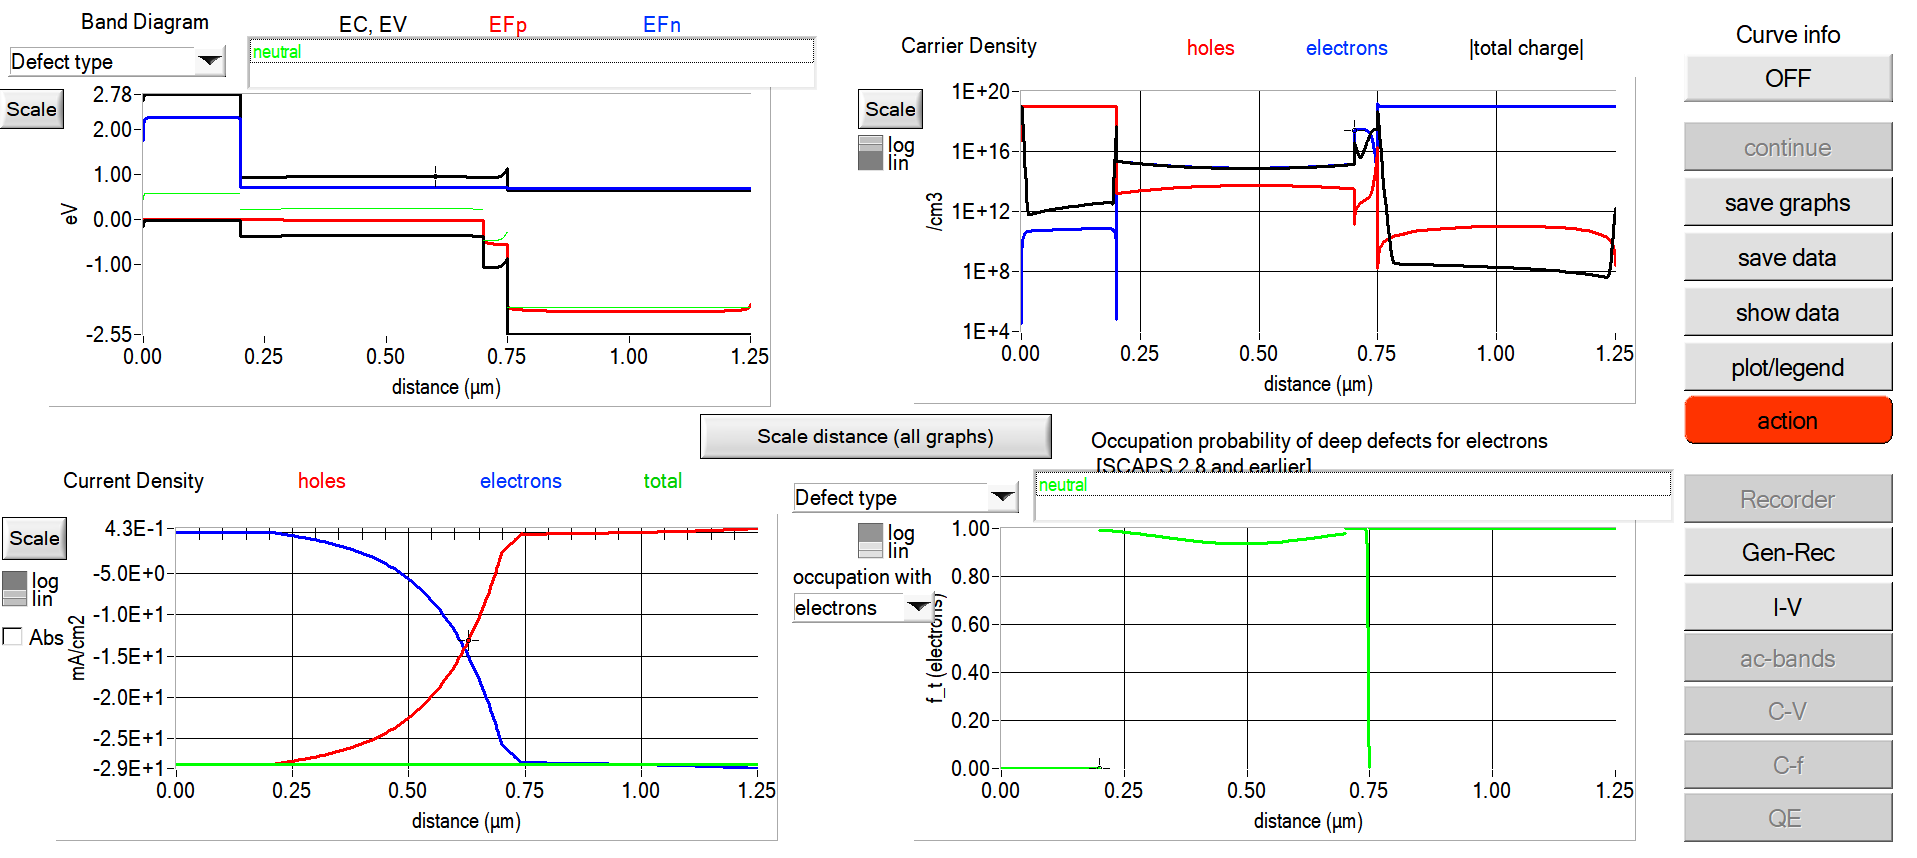
\includegraphics[width=0.85\linewidth]{figs/fig1.png}
\caption{Graphical user interface of SCAPS-1D (version 3.3.10) used for device simulation in this study.}
\end{figure}
Although several SCAPS-1D studies of RbGeI$_{3}$ devices have been reported, most have optimized only a limited subset of device parameters or investigated a single device configuration. The simulation baseline for RbGeI$_{3}$ devices is still low: Pindolia et al. reported a PCE of 9.77\% for the FTO/\allowbreak{}TiO$_{2}$/RbGeI$_{3}$/NiO/\allowbreak{}Ag architecture using SCAPS-1D simulation \cite{r14}. The Pindolia study is broader than its shorthand citation in the secondary literature suggests. The paper systematically studied the effect of various HTL and ETL materials, layer thicknesses, doping concentrations, defect densities, back-contact work functions, and operating temperature in a broad multi-parameter sweep \cite{r14}. Simulation-based studies have since raised the predicted PCE of RbGeI$_{3}$ devices to 27.21\% (2024 \cite{r22}) and 26.47\% (2026 \cite{r23}), although each of these works optimized only a limited subset of device parameters. The ETL--HTL combinations explored for RbGeI$_{3}$ have also been narrow: most studies used TiO$_{2}$ as the ETL and either Spiro-OMeTAD, NiO, or CBTS as the HTL, while the TiO$_{2}$/CuI combination used here has received comparatively little attention despite the well-documented advantages of CuI as an HTL.

\subsection{Contributions and paper organization}
We close this gap by running a SCAPS-1D optimization of an FTO/\allowbreak{}TiO$_{2}$/RbGeI$_{3}$/CuI/\allowbreak{}Au perovskite solar cell. We first screen eight ETL--HTL combinations to identify the FTO/\allowbreak{}TiO$_{2}$/RbGeI$_{3}$/CuI/\allowbreak{}Au architecture as a promising candidate for inorganic-HTL optimization, and then run an eleven-step sequential optimization covering absorber thickness, absorber defect density, dielectric constant, electron affinity, bandgap, conduction- and valence-band effective density of states, ETL and HTL thicknesses, and the two interfacial defect densities. We also analyze the quantum-efficiency spectrum and the equilibrium energy-band diagram of the optimized device, and we benchmark it against recently reported RbGeI$_{3}$-based and related lead-free Ge/Sn-based perovskite solar cells, using primary-source-verified comparator values.
Section II surveys recent literature. Section III describes the device structure and material selection. Section IV presents the methodology and optimization procedure. Section V reports and discusses the results, Section VI compares with prior literature, and Sections VII and VIII cover limitations and conclusions.

\section{Literature Review and Research Gap}
Over the past five years, SCAPS-1D, often combined with first-principles DFT calculations, has become the workhorse numerical tool for designing and optimizing lead-free perovskite solar cells before experimental fabrication. This section surveys the most relevant recent SCAPS-1D studies on Ge-based and Sn-based absorbers, highlighting the device structure, the photovoltaic performance, and the principal limitation of each work. Table I summarizes these studies. All numerical values listed in Table I have been cross-checked against the primary source literature; where a reported efficiency was inconsistent with the device's published J--V metrics, the value implied by those metrics was adopted. In particular, the entries for Pindolia et al. (2022), Loumachi et al. (2024), and Pathak et al. (2026) are quoted verbatim from the corresponding primary sources.

\begin{table}[htbp]
\centering
{\small\setlength{\tabcolsep}{3pt}
\begin{tabularx}{\textwidth}{XXcX}
\hline
Study (Year) [Ref.] & Device Structure & PCE (\%) & Key Limitation
\\\hline
Pindolia et al. (2022) \cite{r14} & FTO/\allowbreak{}TiO$_{2}$/RbGeI$_{3}$/NiO/\allowbreak{}Ag & 9.77 & Broad multi-parameter sweep (HTL, ETL, thickness, doping, defects, back contact, temperature); baseline efficiency remains modest and Ge$^{2+}$ oxidation not addressed.\\
Saikia et al. (2022) \cite{r24} & FTO/\allowbreak{}TiO$_{2}$/CsGeI$_{3}$/CuI/\allowbreak{}Au & 10.80 & No multi-HTL comparative analysis.\\
Bouazizi et al. (2022) \cite{r15} & FTO/\allowbreak{}PCBM/\allowbreak{}CsSn0.5Ge0.5I3/\allowbreak{}Spiro/Au & 18.13 & Mixed Ge/Sn absorber; thermal sensitivity.\\
Loumachi et al. (2024) \cite{r22} & ITO/\allowbreak{}C$_{60}$/RbGeI$_{3}$/CBTS/\allowbreak{}Ag & 27.21 & Optimized RbGeI$_{3}$ thickness and series/shunt resistance; interface defect optimization not addressed.\\
Raj et al. (2025) \cite{r39} & FTO/\allowbreak{}TiO$_{2}$/RbGeI$_{3}$/PEDOT:PSS/\allowbreak{}Au & 18.60 & Organic HTL limits long-term stability.\\
Pathak et al. (2026) \cite{r23} & FTO/\allowbreak{}TiO$_{2}$/RbGeI$_{3}$/Spiro-OMeTAD/\allowbreak{}Au & 26.47 & Ge$^{2+}$ $\rightarrow$ Ge$^{4+}$ oxidation not addressed; only single ETL/HTL combination studied.\\
Dash et al. (2025) \cite{r17} & DFT + SCAPS-1D of RbGeX$_{3}$ (X=Cl, Br, I) & 25.76 & Primarily material-level comparison; limited device-architecture optimization.\\
\hline
\end{tabularx}
}
\caption{Summary of recent SCAPS-1D studies on lead-free Ge-based and Sn-based perovskite solar cells.}
\end{table}
Copper(I) iodide is a wide-gap ($E_{\mathrm{g}}$ $\approx$ 3.1 eV), p-type transparent conductor whose valence-band maximum aligns closely with that of RbGeI$_{3}$, supporting efficient hole extraction \cite{r25,r26}. Reported single-crystal hole mobilities of CuI exceed 100 cm$^{2}$ V$^{-1}$ s$^{-1}$, and the material is solution-processable at low temperatures, which suits large-area fabrication \cite{r27}. Despite these advantages, only a few SCAPS-1D studies have paired CuI with RbGeI$_{3}$, and none has run an eleven-parameter optimization on this combination. Here we vary all eleven device-level parameters on the FTO/\allowbreak{}TiO$_{2}$/RbGeI$_{3}$/CuI/\allowbreak{}Au architecture and report the resulting photovoltaic performance.
A further observation from Table I is that the comparator device structures span a range of ETL and HTL materials (TiO$_{2}$, PCBM, C$_{60}$, NiO, CuI, CBTS, Spiro-OMeTAD, PEDOT:PSS) and back-contact metals (Ag, Au). Two structural details deserve explicit clarification to prevent citation-propagation errors. First, the ETL in the Loumachi et al. device \cite{r22} is C$_{60}$ (buckminsterfullerene), frequently rendered ``C$_{60}$'' in the literature, and the subscript matters because ``C6'' is a different species. Second, the back contact is silver (Ag), not gold (Au), as stated in the primary source \cite{r22}.

\section{Device Structure and Material Selection}

\subsection{Proposed device architecture}
The lead-free perovskite solar cell we propose uses a conventional n-i-p planar heterojunction architecture with the configuration FTO/\allowbreak{}TiO$_{2}$/RbGeI$_{3}$/CuI/\allowbreak{}Au. The device comprises five functional layers: a fluorine-doped tin oxide (FTO) transparent conducting oxide front electrode, a titanium dioxide (TiO$_{2}$) electron transport layer (ETL), a rubidium germanium iodide (RbGeI$_{3}$) absorber layer, a copper iodide (CuI) hole transport layer (HTL), and a gold (Au) back contact. This stack combines efficient charge separation, rapid carrier transport, and suitable energy-level alignment while eliminating the environmental and health concerns associated with lead-based perovskite absorbers. The schematic diagram of the proposed device structure is shown in Figure 2. The choice of constituent materials is justified in the remainder of this section, and the initial material parameters used in the SCAPS-1D simulation are summarized in Table II.

\begin{figure}[htbp]
\centering
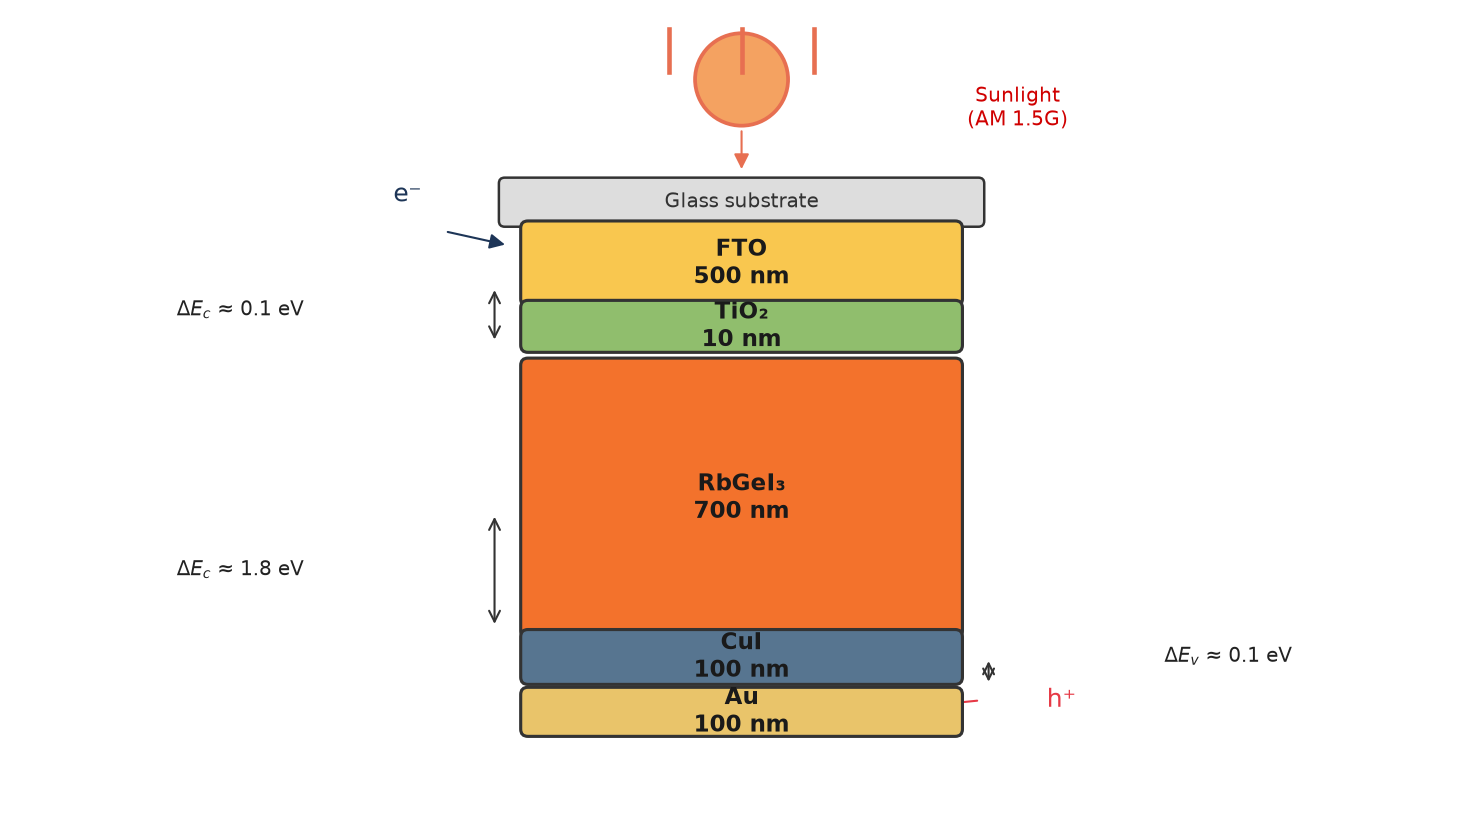
\includegraphics[width=0.85\linewidth]{figs/fig2.png}
\caption{Schematic diagram of the proposed FTO/\allowbreak{}TiO$_{2}$/RbGeI$_{3}$/CuI/\allowbreak{}Au perovskite solar cell structure, showing the five functional layers and the direction of photogenerated carrier transport under AM 1.5G illumination.}
\end{figure}

\subsection{Material selection rationale}
Fluorine-doped tin oxide (FTO) is the front transparent conducting electrode. It has high optical transparency in the visible spectrum together with excellent electrical conductivity, allowing incident sunlight to reach the absorber layer while simultaneously collecting the generated electrons with minimal resistive loss \cite{r28}. FTO was preferred over alternative transparent conducting oxides (such as indium tin oxide, ITO) for its superior thermal and chemical stability, its compatibility with the TiO$_{2}$ ETL deposition process, and its lower cost. The thickness of the FTO layer was fixed at 500 nm, consistent with values commonly reported for perovskite solar cells \cite{r29}.
Titanium dioxide (TiO$_{2}$) is the electron transport layer. The primary function of the ETL is to extract photogenerated electrons from the absorber layer and transport them toward the FTO electrode while effectively blocking holes. TiO$_{2}$ is an n-type semiconductor with a wide bandgap of approximately 3.2 eV in its anatase phase, providing excellent transparency throughout the visible region of the solar spectrum. Its conduction-band minimum lies slightly below that of most iodide-based perovskites, providing an energetically downhill path for photogenerated electrons to transfer from the absorber into the ETL, while its deep valence band acts as an effective barrier against hole transport \cite{r30,r31}. Although its intrinsic electron mobility is lower than that of ZnO and SnO$_{2}$, TiO$_{2}$ provides sufficiently fast electron transport when fabricated with appropriate morphology and crystallinity, and it forms chemically stable interfaces with perovskite materials \cite{r32}.
Rubidium germanium iodide (RbGeI$_{3}$) is the photoactive absorber. Compared with conventional lead-based perovskites, RbGeI$_{3}$ is environmentally friendly because germanium replaces toxic lead while keeping the optoelectronic properties an absorber needs. RbGeI$_{3}$ adopts the ABX$_{3}$ perovskite structure with rubidium at the A-site, germanium at the B-site, and iodine at the X-site. Its direct bandgap in the 1.3--1.4 eV range, strong optical absorption coefficient (reported to be comparable to that of MAPbI$_{3}$ by first-principles calculations \cite{r17,r18}), and good thermal stability make it well-suited for single-junction photovoltaic applications. The initial absorber thickness used for device screening was 400 nm, and the bandgap was initially set to 1.4 eV, consistent with values reported in the experimental literature \cite{r14}. Both parameters were subsequently optimized (Section V).
Copper iodide (CuI) is our hole transport layer, chosen for its excellent hole conductivity, high optical transparency, appropriate valence-band alignment with RbGeI$_{3}$, and comparatively low fabrication cost \cite{r25,r26,r33}. The HTL extracts photogenerated holes efficiently from the absorber layer while preventing electron back-transfer toward the rear electrode. CuI is a wide-gap ($E_{\mathrm{g}}$ $\approx$ 3.1 eV) p-type transparent conductor whose valence-band maximum aligns closely with that of RbGeI$_{3}$ (giving a small valence-band offset of approximately 0.10 eV as quantified in Section V.N), supporting efficient hole extraction. Reported single-crystal hole mobilities of CuI exceed 100 cm$^{2}$ V$^{-1}$ s$^{-1}$, and its solution-processability at low temperatures makes it attractive for large-area fabrication \cite{r27}. The initial CuI thickness was set to 100 nm.
Gold (Au) forms the rear metal contact because of its high work function, excellent electrical conductivity, and superior chemical stability. A high-work-function metal establishes an ohmic contact with the hole transport layer, thereby reducing contact resistance and improving hole collection efficiency \cite{r34}. The choice of Au over lower-work-function alternatives such as Ag or Al ensures that the back contact does not introduce a parasitic Schottky barrier at the CuI/\allowbreak{}Au interface, which would otherwise degrade the fill factor and open-circuit voltage of the device.

\subsection{Initial material parameters}
The initial electrical and optical parameters used in the SCAPS-1D simulation of the proposed FTO/\allowbreak{}TiO$_{2}$/RbGeI$_{3}$/CuI/\allowbreak{}Au solar cell are summarized in Table II. These values were collected from previously published experimental and numerical studies on lead-free perovskite solar cells \cite{r14,r15,r16,r19,r30} and were carefully incorporated into the SCAPS-1D simulator to establish a realistic baseline device before performing further optimization. The interface defect densities applied at the two heterojunctions are listed in Table III. The initial absorber thickness of 400 nm listed in Table II is the value at which all eight device configurations were screened (Section V.A, Table V). This thickness was subsequently optimized to 700 nm in the consolidated final device (Section V.P).

\begin{table}[htbp]
\centering
{\footnotesize\setlength{\tabcolsep}{3pt}
\begin{tabularx}{\textwidth}{Xcccc}
\hline
Parameter & TiO$_{2}$ & FTO & RbGeI$_{3}$ & CuI
\\\hline
Thickness (nm) & 30 & 500 & 400 & 100\\
Bandgap $E_{\mathrm{g}}$ (eV) & 3.2 & 3.2 & 1.4 & 3.1\\
Electron affinity $\chi$ (eV) & 4.0 & 4.4 & 3.9 & 2.1\\
Dielectric permittivity $\epsilon$r & 9 & 9 & 23.01 & 6.5\\
CB effective DOS N$_{\mathrm{C}}$ (cm$^{-3}$) & 2$\times$10$^{18}$ & 2.2$\times$10$^{18}$ & 1.4$\times$10$^{19}$ & 2.8$\times$10$^{19}$\\
VB effective DOS N$_{\mathrm{V}}$ (cm$^{-3}$) & 1.8$\times$10$^{19}$ & 1.8$\times$10$^{19}$ & 2.8$\times$10$^{19}$ & 1$\times$10$^{19}$\\
Electron mobility $\mu$e (cm$^{2}$ V$^{-1}$ s$^{-1}$) & 20 & 20 & 28.6 & 100\\
Hole mobility $\mu$p (cm$^{2}$ V$^{-1}$ s$^{-1}$) & 10 & 10 & 27.3 & 43.9\\
Donor density $N_{\mathrm{D}}$ (cm$^{-3}$) & 9$\times$10$^{16}$ & 1$\times$10$^{19}$ & 1$\times$10$^{9}$ & 0\\
Acceptor density $N_{\mathrm{A}}$ (cm$^{-3}$) & 0 & 0 & 1$\times$10$^{9}$ & 1$\times$10$^{18}$\\
Bulk defect density $N_{\mathrm{t}}$ (cm$^{-3}$) & 1$\times$10$^{15}$ & 1$\times$10$^{14}$ & 1$\times$10$^{15}$ & 1$\times$10$^{15}$\\
\hline
\end{tabularx}
}
\caption{Initial electrical and optical parameters used in the SCAPS-1D simulation of the proposed FTO/\allowbreak{}TiO$_{2}$/RbGeI$_{3}$/CuI/\allowbreak{}Au solar cell.}
\end{table}

\begin{table}[htbp]
\centering
{\small\setlength{\tabcolsep}{3pt}
\begin{tabularx}{\textwidth}{Xc}
\hline
Interface & Interface defect density $N_{\mathrm{t}}$ (cm$^{-2}$)
\\\hline
TiO$_{2}$ / RbGeI$_{3}$ & 1 $\times$ 10$^{14}$\\
RbGeI$_{3}$ / CuI & 1 $\times$ 10$^{14}$\\
\hline
\end{tabularx}
}
\caption{Initial interface defect density applied at each heterojunction.}
\end{table}

\section{Methodology}

\subsection{SCAPS-1D simulation framework}
The device stack was simulated with SCAPS-1D version 3.3.10 \cite{r19,r20,r21}, which solves the Poisson equation together with the electron and hole continuity equations self-consistently across the device and is widely used for thin-film and perovskite device studies. The drift-diffusion transport model underlying these equations is summarized below; further details are available in the original references \cite{r19,r20,r21}.
\begin{equation}\label{eq:poisson}
\frac{d}{dx}\left(\epsilon\frac{d\psi}{dx}\right) =
-q\left(p-n+N_{D}-N_{A}+\rho_{t}\right)
\end{equation}
\begin{equation}\label{eq:electron}
\frac{dJ_{n}}{dx} = q\,(R-G)
\end{equation}
\begin{equation}\label{eq:hole}
\frac{dJ_{p}}{dx} = q\,(G-R)
\end{equation}
where $\epsilon$ is the dielectric permittivity, $\psi$ the electrostatic potential, q the elementary charge, n and p the electron and hole concentrations, $N_{\mathrm{D}}$ and $N_{\mathrm{A}}$ the donor and acceptor concentrations, and $\rho_{\mathrm{t}}$ the trapped charge density. Electron and hole transport are governed by the continuity equations,
where $J_{\mathrm{n}}$ is the electron current density, G the carrier generation rate, and R the carrier recombination rate; the hole continuity equation describes hole transport analogously,
where $J_{\mathrm{p}}$ is the hole current density. Together, Eqs. (1)--(3) describe generation, transport, and recombination under illumination; SCAPS-1D computes the resulting J--V characteristics from the layer properties defined below.

\subsection{Simulation conditions}
All simulations were performed under the AM 1.5G spectrum at an incident power density of 100 mW/cm$^{2}$ (one sun, STC) with the operating temperature fixed at 300 K, using the initial material parameters of Table II and the interface defect densities of Table III unless otherwise stated. During each optimization step, only one parameter was varied while all remaining parameters were held constant; the general simulation conditions are summarized in Table IV. Absorption uses the SCAPS square-root law $\alpha$ = A$\sqrt{h\nu-E_{\mathrm{g}}}$ with A = 10$^{5}$ cm$^{-1}$ (uniform at the electrical bandgap). Contacts are ideal ($R_{\mathrm{s}}$ = 0, $R_{\mathrm{sh}}$ = $\infty$); no series/shunt resistance is included unless stated, so fill factors are upper bounds. Figures 3--13 record each sweep as-run with its contemporary deck version; absolute offsets between sweep generations (e.g. the Section V.B sweep record) are bounded by consolidated-deck re-simulation, and all headline metrics come solely from single consolidated-deck runs.

\begin{table}[htbp]
\centering
{\small\setlength{\tabcolsep}{3pt}
\begin{tabularx}{\textwidth}{XX}
\hline
Parameter & Value
\\\hline
Simulation software & SCAPS-1D version 3.3.10\\
Illumination spectrum & AM 1.5G\\
Incident power density & 100 mW/cm$^{2}$ (1000 W/m$^{2}$)\\
Operating temperature & 300 K (27 $^{\circ}$C)\\
Illumination intensity & 1 Sun\\
Scan mode & Illuminated J--V\\
Device type & Planar heterojunction\\
Front contact & FTO\\
Back contact & Au\\
Initial material parameters & Table II\\
Initial interface defect density & Table III\\
\hline
\end{tabularx}
}
\caption{Simulation conditions used in SCAPS-1D.}
\end{table}

\subsection{Performance parameters}
Performance was evaluated using the four key parameters extracted from the simulated J--V curve: open-circuit voltage (V$_{\mathrm{OC}}$), short-circuit current density (J$_{\mathrm{SC}}$), fill factor (FF), and power conversion efficiency (PCE), computed as PCE = (V$_{\mathrm{OC}}$ $\times$ J$_{\mathrm{SC}}$ $\times$ FF)/Pin with Pin = 100 mW/cm$^{2}$ under AM 1.5G.

\subsection{Sequential optimization procedure}
Starting from the initial device, one parameter at a time (OPAT) was varied while all others were held constant, and each step's locally optimal value was carried forward into the subsequent step, as detailed in Section V.
The procedure comprises eleven optimization steps: (1) absorber thickness (0.3--1.0 $\mu$m); (2) absorber bulk defect density (10$^{12}$--10$^{18}$ cm$^{-3}$); (3) absorber dielectric constant (15--23.1); (4) absorber electron affinity (3.9--4.2 eV); (5) TiO$_{2}$/RbGeI$_{3}$ interfacial defect density (10$^{12}$--10$^{18}$ cm$^{-2}$); (6) RbGeI$_{3}$/CuI interfacial defect density (10$^{12}$--10$^{18}$ cm$^{-2}$); (7) absorber bandgap (1.3--1.7 eV); (8) TiO$_{2}$ ETL thickness (0.01--0.09 $\mu$m); (9) CuI HTL thickness (0.1--1.9 $\mu$m); (10) conduction-band effective density of states N$_{\mathrm{C}}$ (1$\times$10$^{17}$--1$\times$10$^{20}$ cm$^{-3}$); (11) valence-band effective density of states N$_{\mathrm{V}}$ (1$\times$10$^{17}$--1$\times$10$^{20}$ cm$^{-3}$). Each step's locally optimal parameter value was carried forward into all subsequent steps, with the consolidated final parameter set summarized in Table VII.
Because each per-step optimum is identified with all other parameters fixed at prior-step values, the consolidated parameter set may not be a global optimum; the OPAT approach nevertheless identifies the dominant parameter effects and establishes a clear baseline. To test for missed cross-interactions, Section V.P reports a genetic-algorithm (GA) joint optimization over the six most sensitive parameters (bandgap, bulk and interface defect densities, N$_{\mathrm{C}}$, N$_{\mathrm{V}}$, absorber thickness), which finds a higher mathematical optimum at a lower bandgap and lower defect density than the OPAT point.

\subsection{Device configurations screened}
Eight planar configurations combining two ETLs (TiO$_{2}$, PCBM) with four HTLs (NiO, CuI, CBTS, Spiro-OMeTAD) around the RbGeI$_{3}$ absorber (D1--D8, Table V) were simulated at the initial absorber thickness of 400 nm (Table II) to permit a fair architecture comparison before the thickness optimization of Section V.B.

\begin{table}[htbp]
\centering
{\small\setlength{\tabcolsep}{3pt}
\begin{tabularx}{\textwidth}{XX}
\hline
Device & Architecture
\\\hline
D1 & FTO / PCBM / RbGeI$_{3}$ / NiO / Au\\
D2 & FTO / TiO$_{2}$ / RbGeI$_{3}$ / NiO / Au\\
D3 & FTO / PCBM / RbGeI$_{3}$ / CuI / Au\\
D4 & FTO / TiO$_{2}$ / RbGeI$_{3}$ / CuI / Au\\
D5 & FTO / PCBM / RbGeI$_{3}$ / CBTS / Au\\
D6 & FTO / TiO$_{2}$ / RbGeI$_{3}$ / CBTS / Au\\
D7 & FTO / PCBM / RbGeI$_{3}$ / Spiro-OMeTAD / Au\\
D8 & FTO / TiO$_{2}$ / RbGeI$_{3}$ / Spiro-OMeTAD / Au\\
\hline
\end{tabularx}
}
\caption{Eight device configurations screened in this study. All configurations were simulated at an absorber thickness of 400 nm.}
\end{table}

\section{Results and Discussion}

\subsection{Screening of device configurations}
Table VI compiles the photovoltaics of all eight configurations: two ETLs (TiO$_{2}$, PCBM) crossed with four HTLs (NiO, CuI, CBTS, Spiro-OMeTAD) on the common RbGeI$_{3}$ absorber.
The D4 architecture (TiO$_{2}$/CuI) combines well-matched band alignment with an all-inorganic transport stack, avoiding the stability limitations of organic HTLs.

\begin{table}[htbp]
\centering
{\footnotesize\setlength{\tabcolsep}{3pt}
\begin{tabularx}{\textwidth}{XXcccc}
\hline
Dev. & Architecture & V$_{\mathrm{OC}}$ (V) & J$_{\mathrm{SC}}$ (mA/cm$^{2}$) & FF (\%) & PCE (\%)
\\\hline
D1 & FTO/\allowbreak{}PCBM/\allowbreak{}RbGeI$_{3}$/NiO/\allowbreak{}Au & 0.81 & 30.10 & 83.68 & 20.40\\
D2 & FTO/\allowbreak{}TiO$_{2}$/RbGeI$_{3}$/NiO/\allowbreak{}Au & 0.82 & 30.46 & 84.48 & 21.10\\
D3 & FTO/\allowbreak{}PCBM/\allowbreak{}RbGeI$_{3}$/CuI/\allowbreak{}Au & 0.81 & 30.10 & 83.96 & 20.47\\
D4 & FTO/\allowbreak{}TiO$_{2}$/RbGeI$_{3}$/CuI/\allowbreak{}Au & 0.812 & 30.46 & 79.98 & 19.78\\
D5 & FTO/\allowbreak{}PCBM/\allowbreak{}RbGeI$_{3}$/CBTS/\allowbreak{}Au & 0.82 & 30.20 & 82.36 & 20.40\\
D6 & FTO/\allowbreak{}TiO$_{2}$/RbGeI$_{3}$/CBTS/\allowbreak{}Au & 0.82 & 30.55 & 82.13 & 20.57\\
D7 & FTO/\allowbreak{}PCBM/\allowbreak{}RbGeI$_{3}$/Spiro/Au & 0.81 & 30.07 & 85.01 & 20.71\\
D8 & FTO/\allowbreak{}TiO$_{2}$/RbGeI$_{3}$/Spiro/Au & 0.82 & 30.46 & 83.95 & 20.97\\
\hline
\end{tabularx}
}
\caption{Initial photovoltaic performance of the eight screened device configurations, simulated at an absorber thickness of 400 nm.  Selected as the baseline for full parametric optimization.}
\end{table}
The best FF belongs to D7 (Spiro-OMeTAD, 85.01\%) and the best PCE to D2 (21.10\%), not to D4. D4 still won our attention: CuI beats Spiro-OMeTAD on stability and cost and NiO on moisture and oxygen sensitivity while offering higher hole mobility. Its PCE deficit of about 1.3 percentage points to the top entries is the kind of gap the parameter sweep can close; the stability and cost that CuI carries are not something parameter tuning can buy back.

\subsection{Effect of absorber layer thickness}
Thickness sets the trade-off between light capture and recombination: a thicker absorber absorbs more photons and lifts J$_{\mathrm{SC}}$, up to the point where the extra volume becomes a recombination liability.
PCE peaks at 0.7 $\mu$m (20.70\%) and eases off beyond it as recombination grows. J$_{\mathrm{SC}}$ climbs steadily with thickness, 28.14 to 34.11 mA/cm$^{2}$, while V$_{\mathrm{OC}}$ slides from 0.823 to 0.767 V. The 0.7 $\mu$m point, where the two effects balance, is the one we keep. The upper end of this J$_{\mathrm{SC}}$ range (34.11 mA/cm$^{2}$) exceeds the single-gap SQ limit at 1.4 eV ($\approx$33 mA/cm$^{2}$); it was recorded with the early Step-1 deck whose extended sub-gap absorption (cutoff toward $\approx$1.2 eV, SQ $\approx$40 mA/cm$^{2}$) accommodates it. Re-simulation of the thickness sweep with the consolidated uniform-1.4 eV deck gives J$_{\mathrm{SC}}$ 25.2--31.3 mA/cm$^{2}$ (all below SQ) with the same peak-plateau shape (plateau 0.7--1.0 $\mu$m within 0.06 points), so the 0.7 $\mu$m choice stands.

\begin{figure}[htbp]
\centering
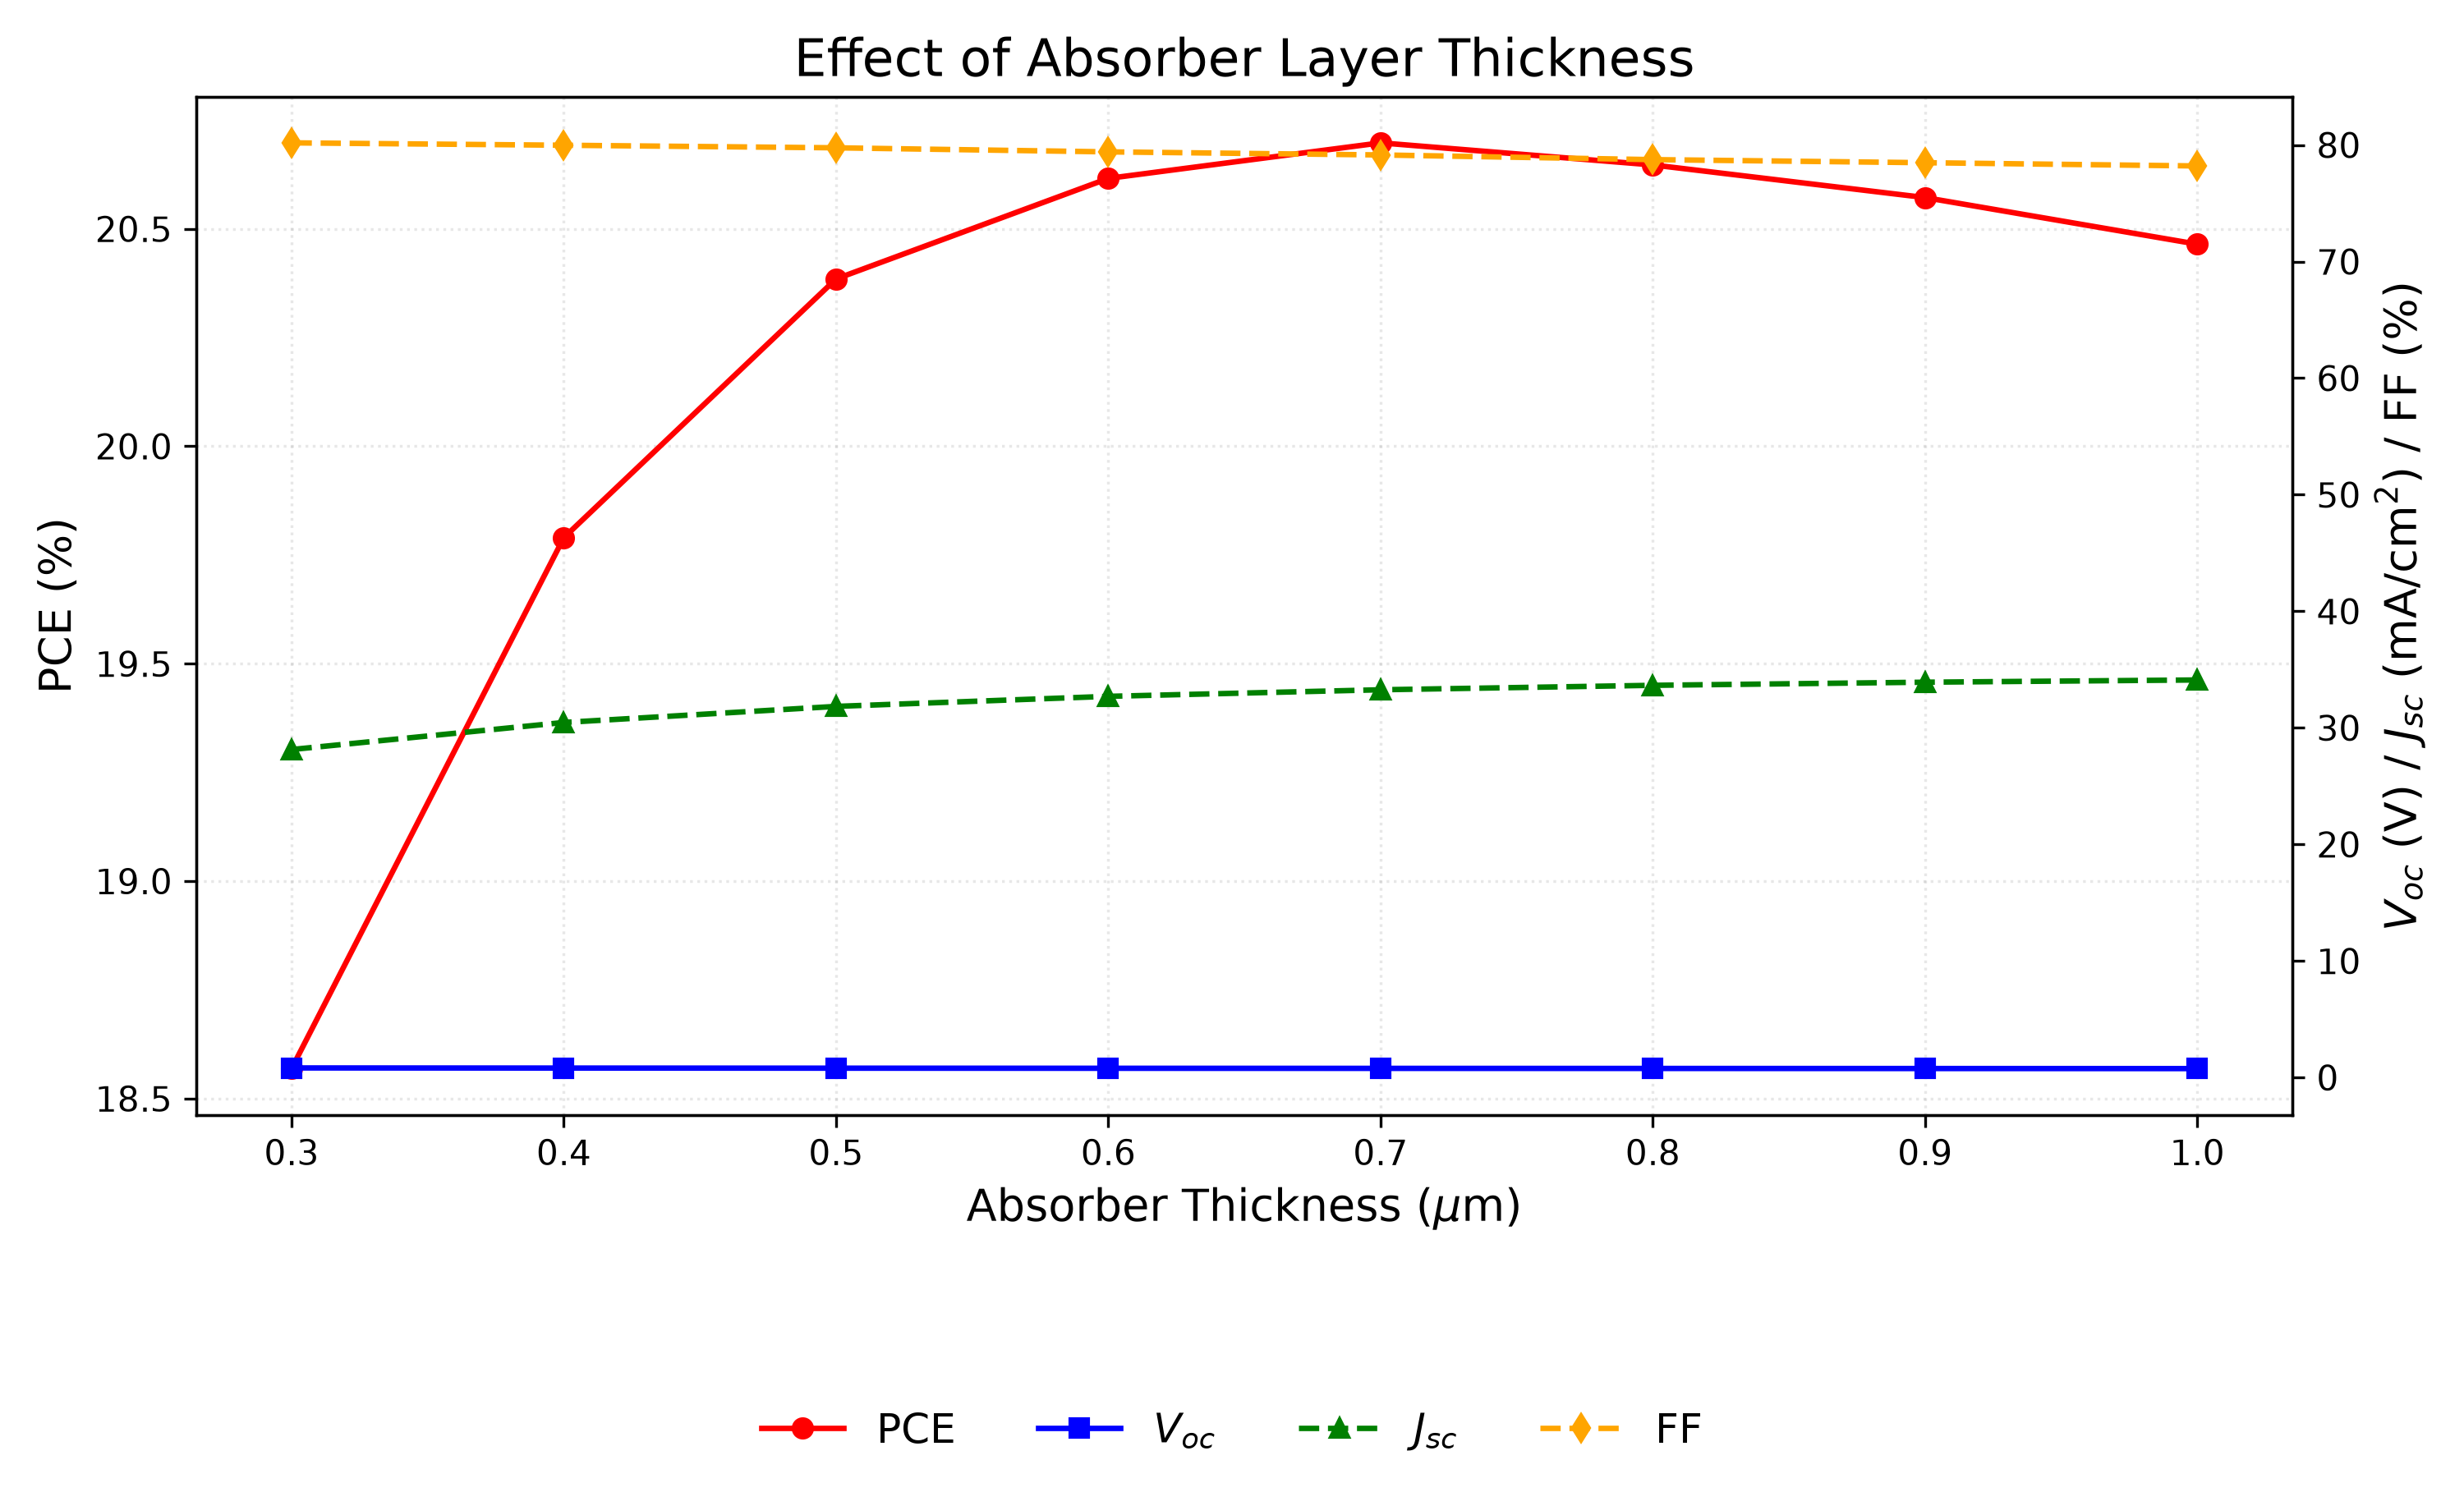
\includegraphics[width=0.85\linewidth]{figs/fig3.png}
\caption{Variation of PCE, V$_{\mathrm{OC}}$, J$_{\mathrm{SC}}$, and FF with RbGeI$_{3}$ absorber thickness. PCE peaks at 0.7 $\mu$m, beyond which recombination losses reduce efficiency.}
\end{figure}

\subsection{Effect of absorber defect density}
In the bulk, defects shorten carrier lifetimes and cut collection efficiency by acting as Shockley-Read-Hall (SRH) recombination centers. We swept the RbGeI$_{3}$ defect density from 10$^{12}$ to 10$^{18}$ cm$^{-3}$ with all else fixed.
The device tolerates defects up to 10$^{14}$ cm$^{-3}$ without visible loss; above that, PCE collapses from 20.40\% to 7.58\% as the density reaches 10$^{18}$ cm$^{-3}$, mostly through falling V$_{\mathrm{OC}}$ (0.848 to 0.550 V). The sweep settles at 10$^{14}$ cm$^{-3}$, the bulk density SCAPS studies typically assume for lead-free absorbers.
Beyond the total trap density, the energetic position $E_{\mathrm{t}}$ of the dominant defect and the electron/hole capture asymmetry ($\sigma_{n}$, $\sigma_{p}$) were swept to model Ge-related degradation explicitly. At $N_{\mathrm{t}}$ = $10^{15}$ cm$^{-3}$, moving $E_{\mathrm{t}}$ from 0.2 eV to 1.2 eV above $E_{\mathrm{v}}$ traces a shallow symmetric minimum centred at mid-gap: PCE falls from 25.01\% at the band edges to 24.84\% for $E_{\mathrm{t}}$ = 0.4-1.0 eV (Fig. 24), the textbook SRH fingerprint that mid-gap states are the most lethal recombination centres. At the baseline $N_{\mathrm{t}}$ = $10^{14}$ cm$^{-3}$ the level position is immaterial (26.81-26.85\%), confirming the consolidated defect budget sits deep inside the tolerant regime. Capture asymmetry at mid-gap (Fig. 25) is significant even at a fixed $\sigma_{n}\times\sigma_{p}$ product: the electron-capture-dominated trap ($\sigma_{n}$ = $10^{-17}$, $\sigma_{p}$ = $10^{-19}$ m2) limits PCE to 23.97\%, while the mirrored hole-dominated trap holds 26.71\%, and the symmetric $10^{-17}$/$10^{-17}$ case collapses to 21.45\%. The oxidation threat (Ge$^{2+}$ $\rightarrow$ Ge$^{4+}$, Ge vacancies) therefore cannot be reduced to a single $N_{\mathrm{t}}$ number: its energy and capture character jointly set the damage, and dense symmetric traps are the worst case.

\begin{figure}[htbp]
\centering
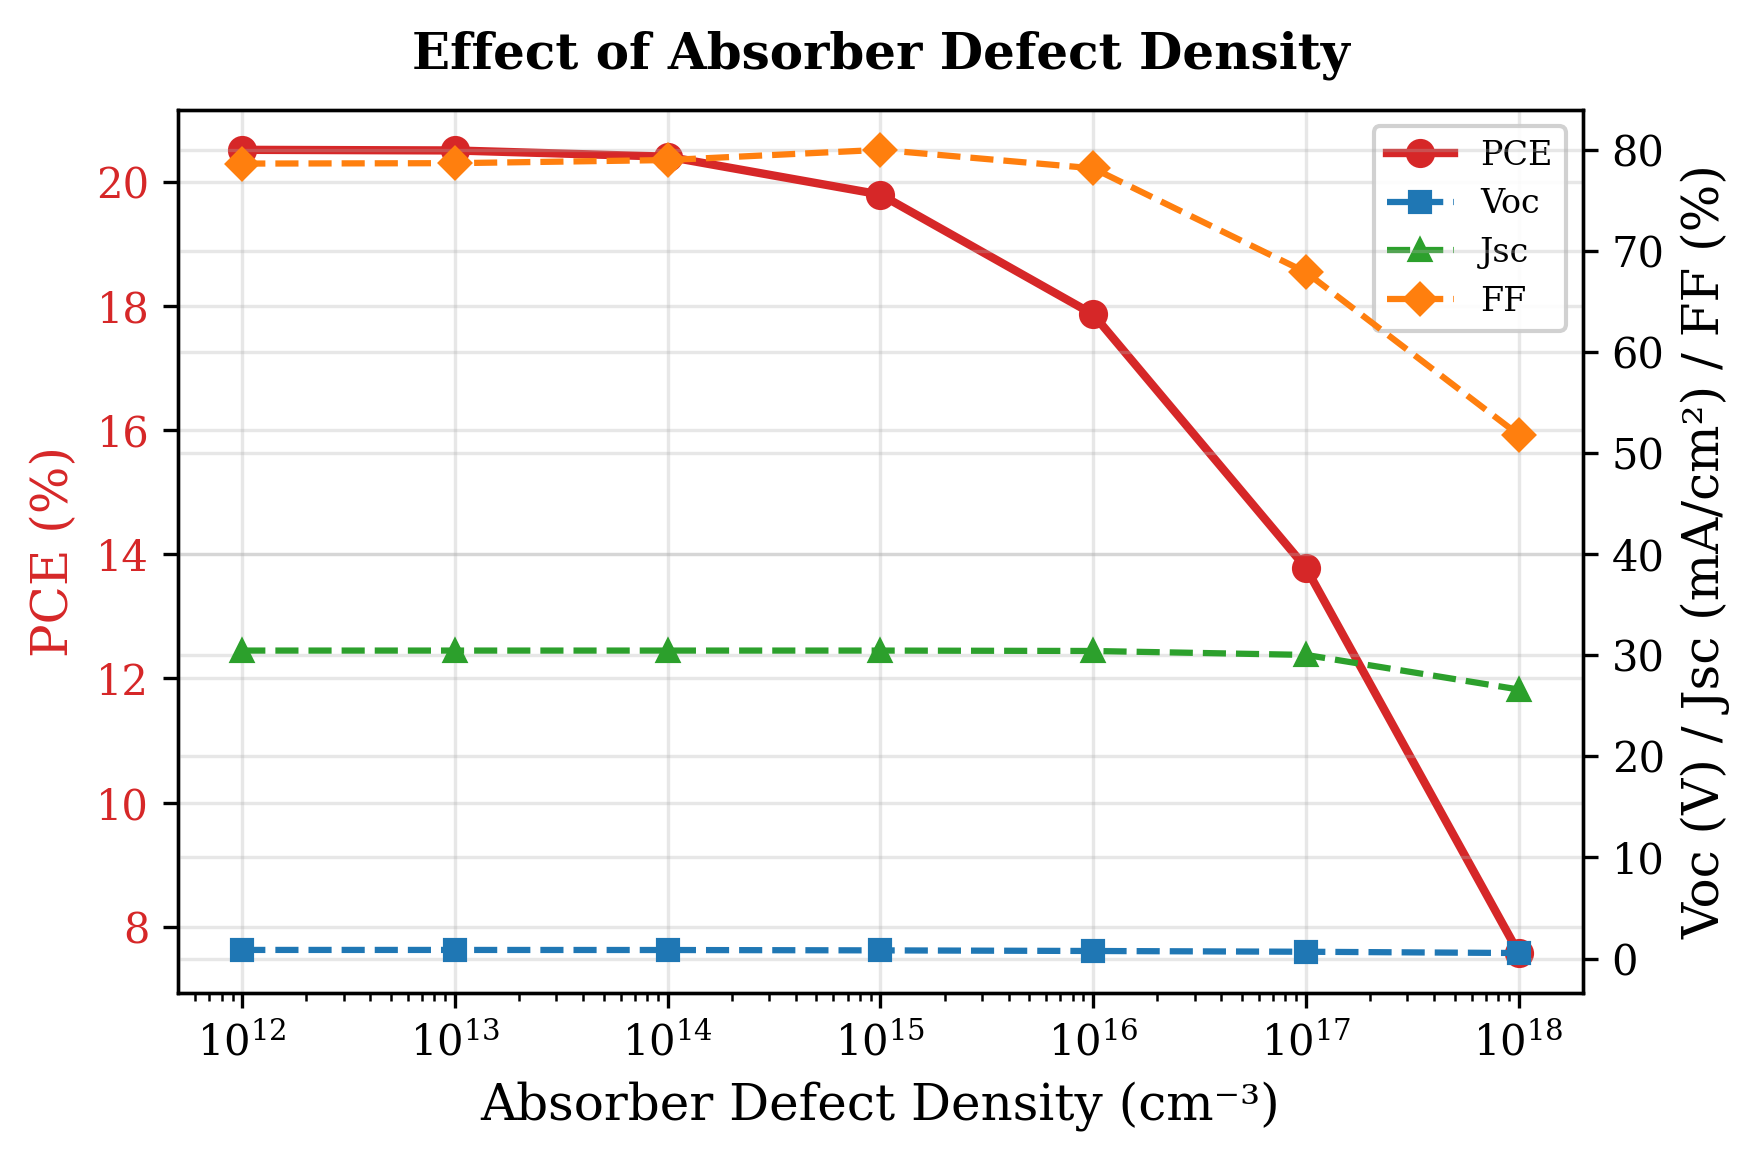
\includegraphics[width=0.85\linewidth]{figs/fig4.png}
\caption{Variation of PCE, V$_{\mathrm{OC}}$, J$_{\mathrm{SC}}$, and FF with RbGeI$_{3}$ absorber defect density. Performance degrades sharply above 10$^{14}$ cm$^{-3}$.}
\end{figure}

\subsection{Effect of absorber dielectric constant}
The dielectric constant barely matters. Raising $\epsilon$r from 15 to 23.1 moves PCE from 19.92\% to 19.79\%, a shift carried almost entirely by V$_{\mathrm{OC}}$ (0.819 to 0.812 V); J$_{\mathrm{SC}}$ and FF are essentially unchanged. With nothing to gain at the high end, we keep $\epsilon$r = 15.

\begin{figure}[htbp]
\centering
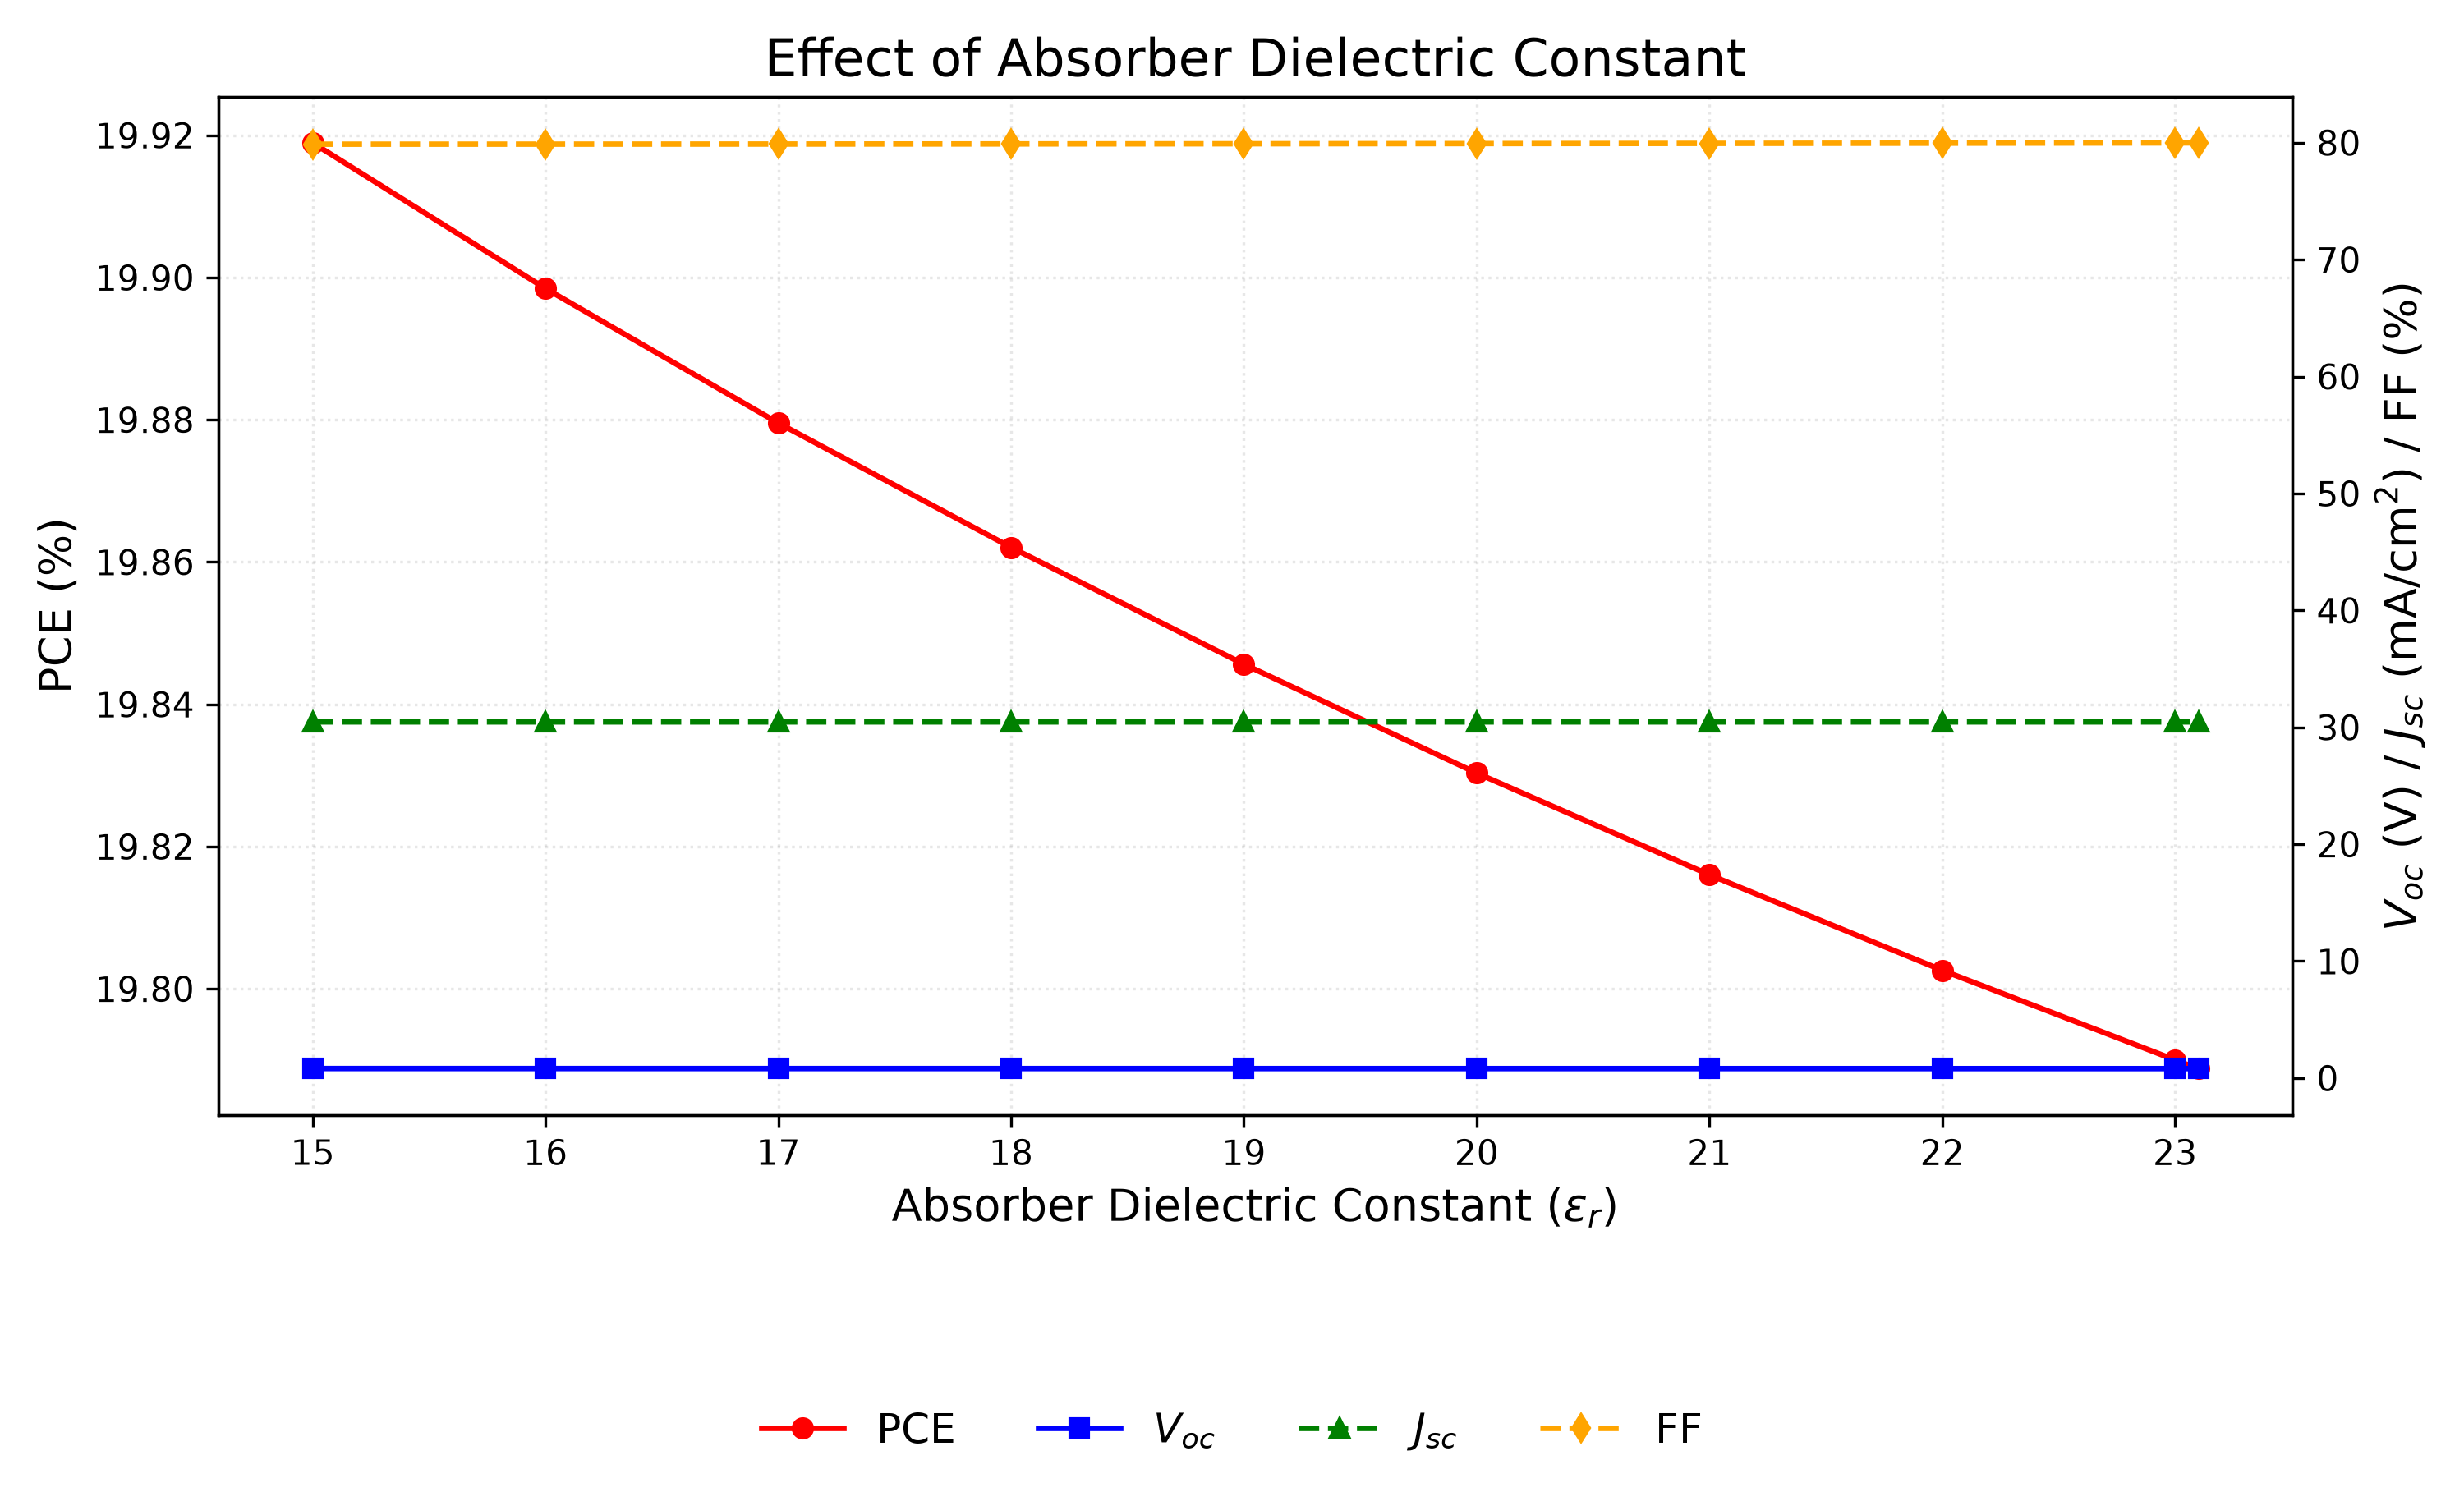
\includegraphics[width=0.85\linewidth]{figs/fig5.png}
\caption{Variation of PCE, V$_{\mathrm{OC}}$, J$_{\mathrm{SC}}$, and FF with RbGeI$_{3}$ absorber dielectric constant. The performance is essentially insensitive to $\epsilon$r across the investigated range; $\epsilon$r = 15 is used in the final device.}
\end{figure}

\subsection{Effect of absorber electron affinity}
Electron affinity lines up the energy bands between adjacent layers and so controls extraction of the charge carriers. We held everything else fixed and stepped $\chi$ from 3.9 to 4.2 eV.
Peak performance lands at $\chi$ = 3.9 eV with a PCE of 19.79\%. Raise the affinity to 4.2 eV and V$_{\mathrm{OC}}$ falls from 0.812 to 0.710 V while J$_{\mathrm{SC}}$ holds flat: the extra electron affinity buys a fill-factor gain smaller than the voltage it costs. We stay at 3.9 eV.

\begin{figure}[htbp]
\centering
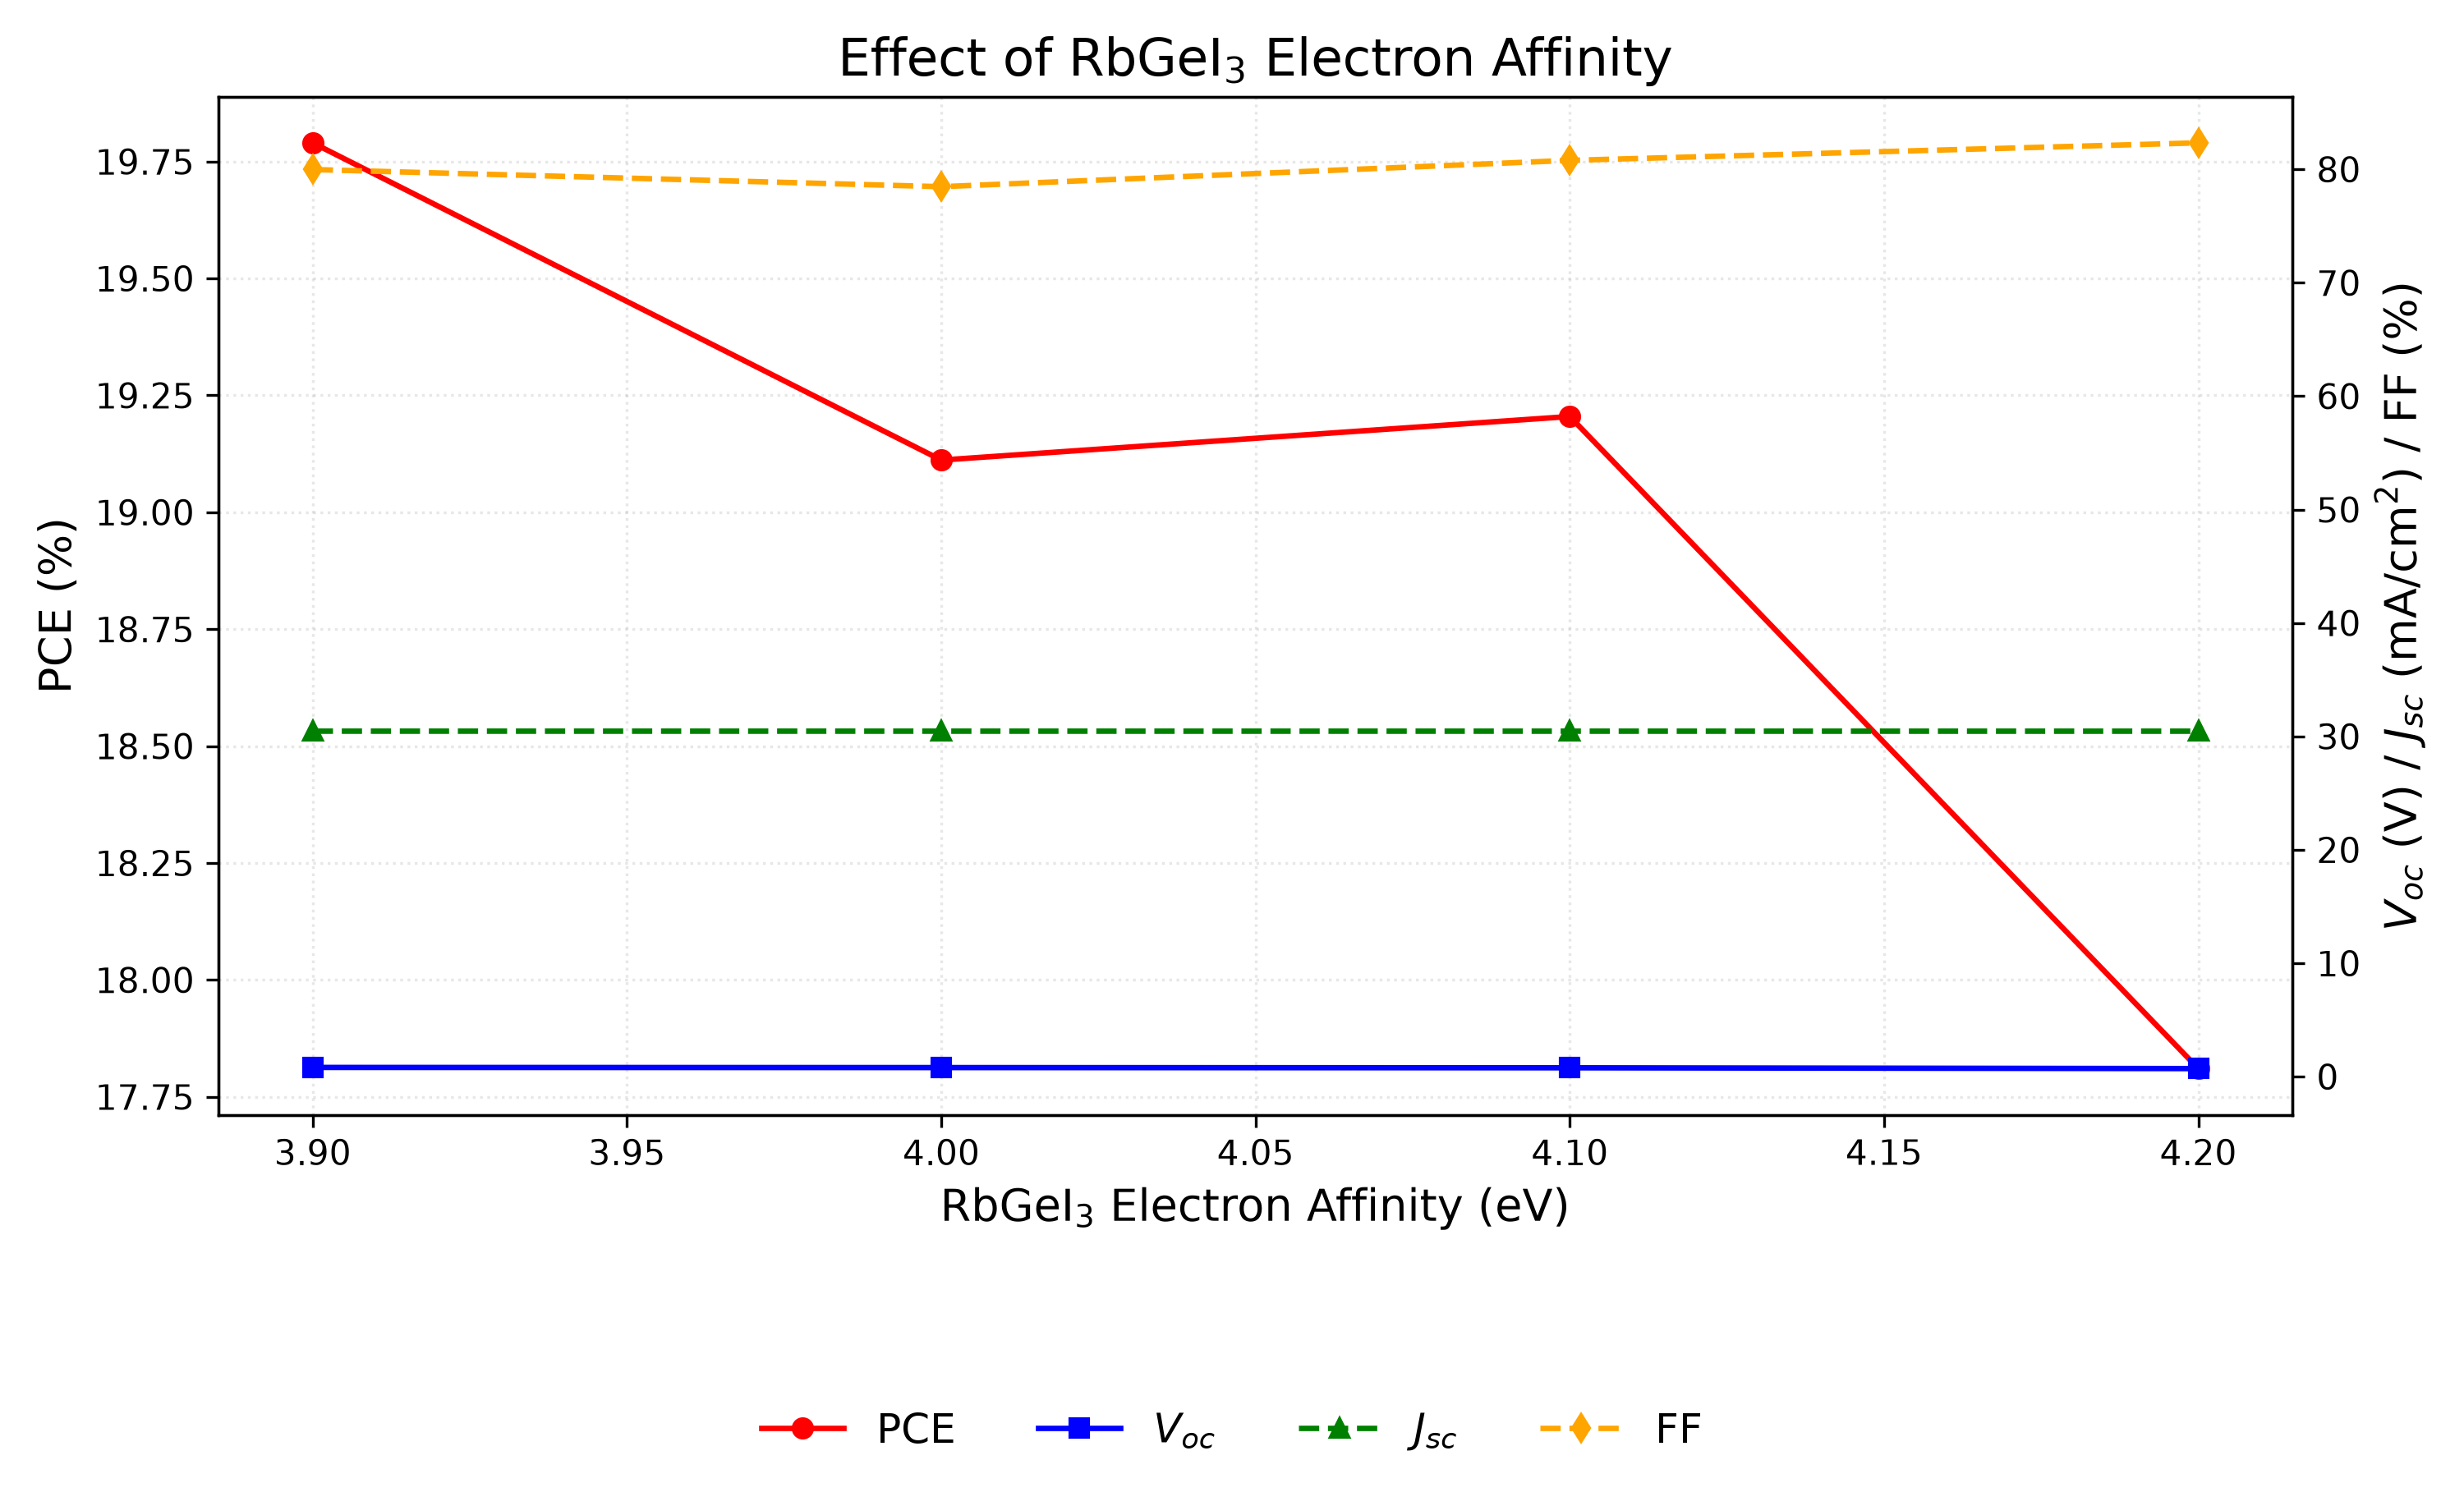
\includegraphics[width=0.85\linewidth]{figs/fig6.png}
\caption{Variation of PCE, V$_{\mathrm{OC}}$, J$_{\mathrm{SC}}$, and FF with RbGeI$_{3}$ absorber electron affinity. PCE is highest at $\chi$ = 3.9 eV due to optimal band alignment with TiO$_{2}$.}
\end{figure}

\subsection{Effect of TiO$_{2}$/RbGeI$_{3}$ interfacial defect density}
The TiO$_{2}$/RbGeI$_{3}$ interface is where performance is won or lost. Varying its defect density from 10$^{12}$ to 10$^{18}$ cm$^{-2}$, with everything else fixed, sends the device off a cliff: PCE drops from 21.04\% to 8.40\%, V$_{\mathrm{OC}}$ from 0.827 to 0.439 V, J$_{\mathrm{SC}}$ from 30.46 to 28.09 mA/cm$^{2}$, and FF from 83.52\% to 68.11\% (Figure 7).
More states at the TiO$_{2}$/RbGeI$_{3}$ junction mean more carriers captured before they reach the electrodes; V$_{\mathrm{OC}}$, J$_{\mathrm{SC}}$, and FF fall together. Best performance comes at the unphysical 10$^{12}$ cm$^{-2}$ floor, but the final device targets 10$^{14}$ cm$^{-2}$, a density a real film can hit and keep: Ge$^{2+}$ oxidation and moisture sensitivity during preparation make anything below that hard to hold consistently. The figure also matches the bulk density chosen in Section V.C and the value comparable SCAPS studies of lead-free perovskites assume.

\begin{figure}[htbp]
\centering
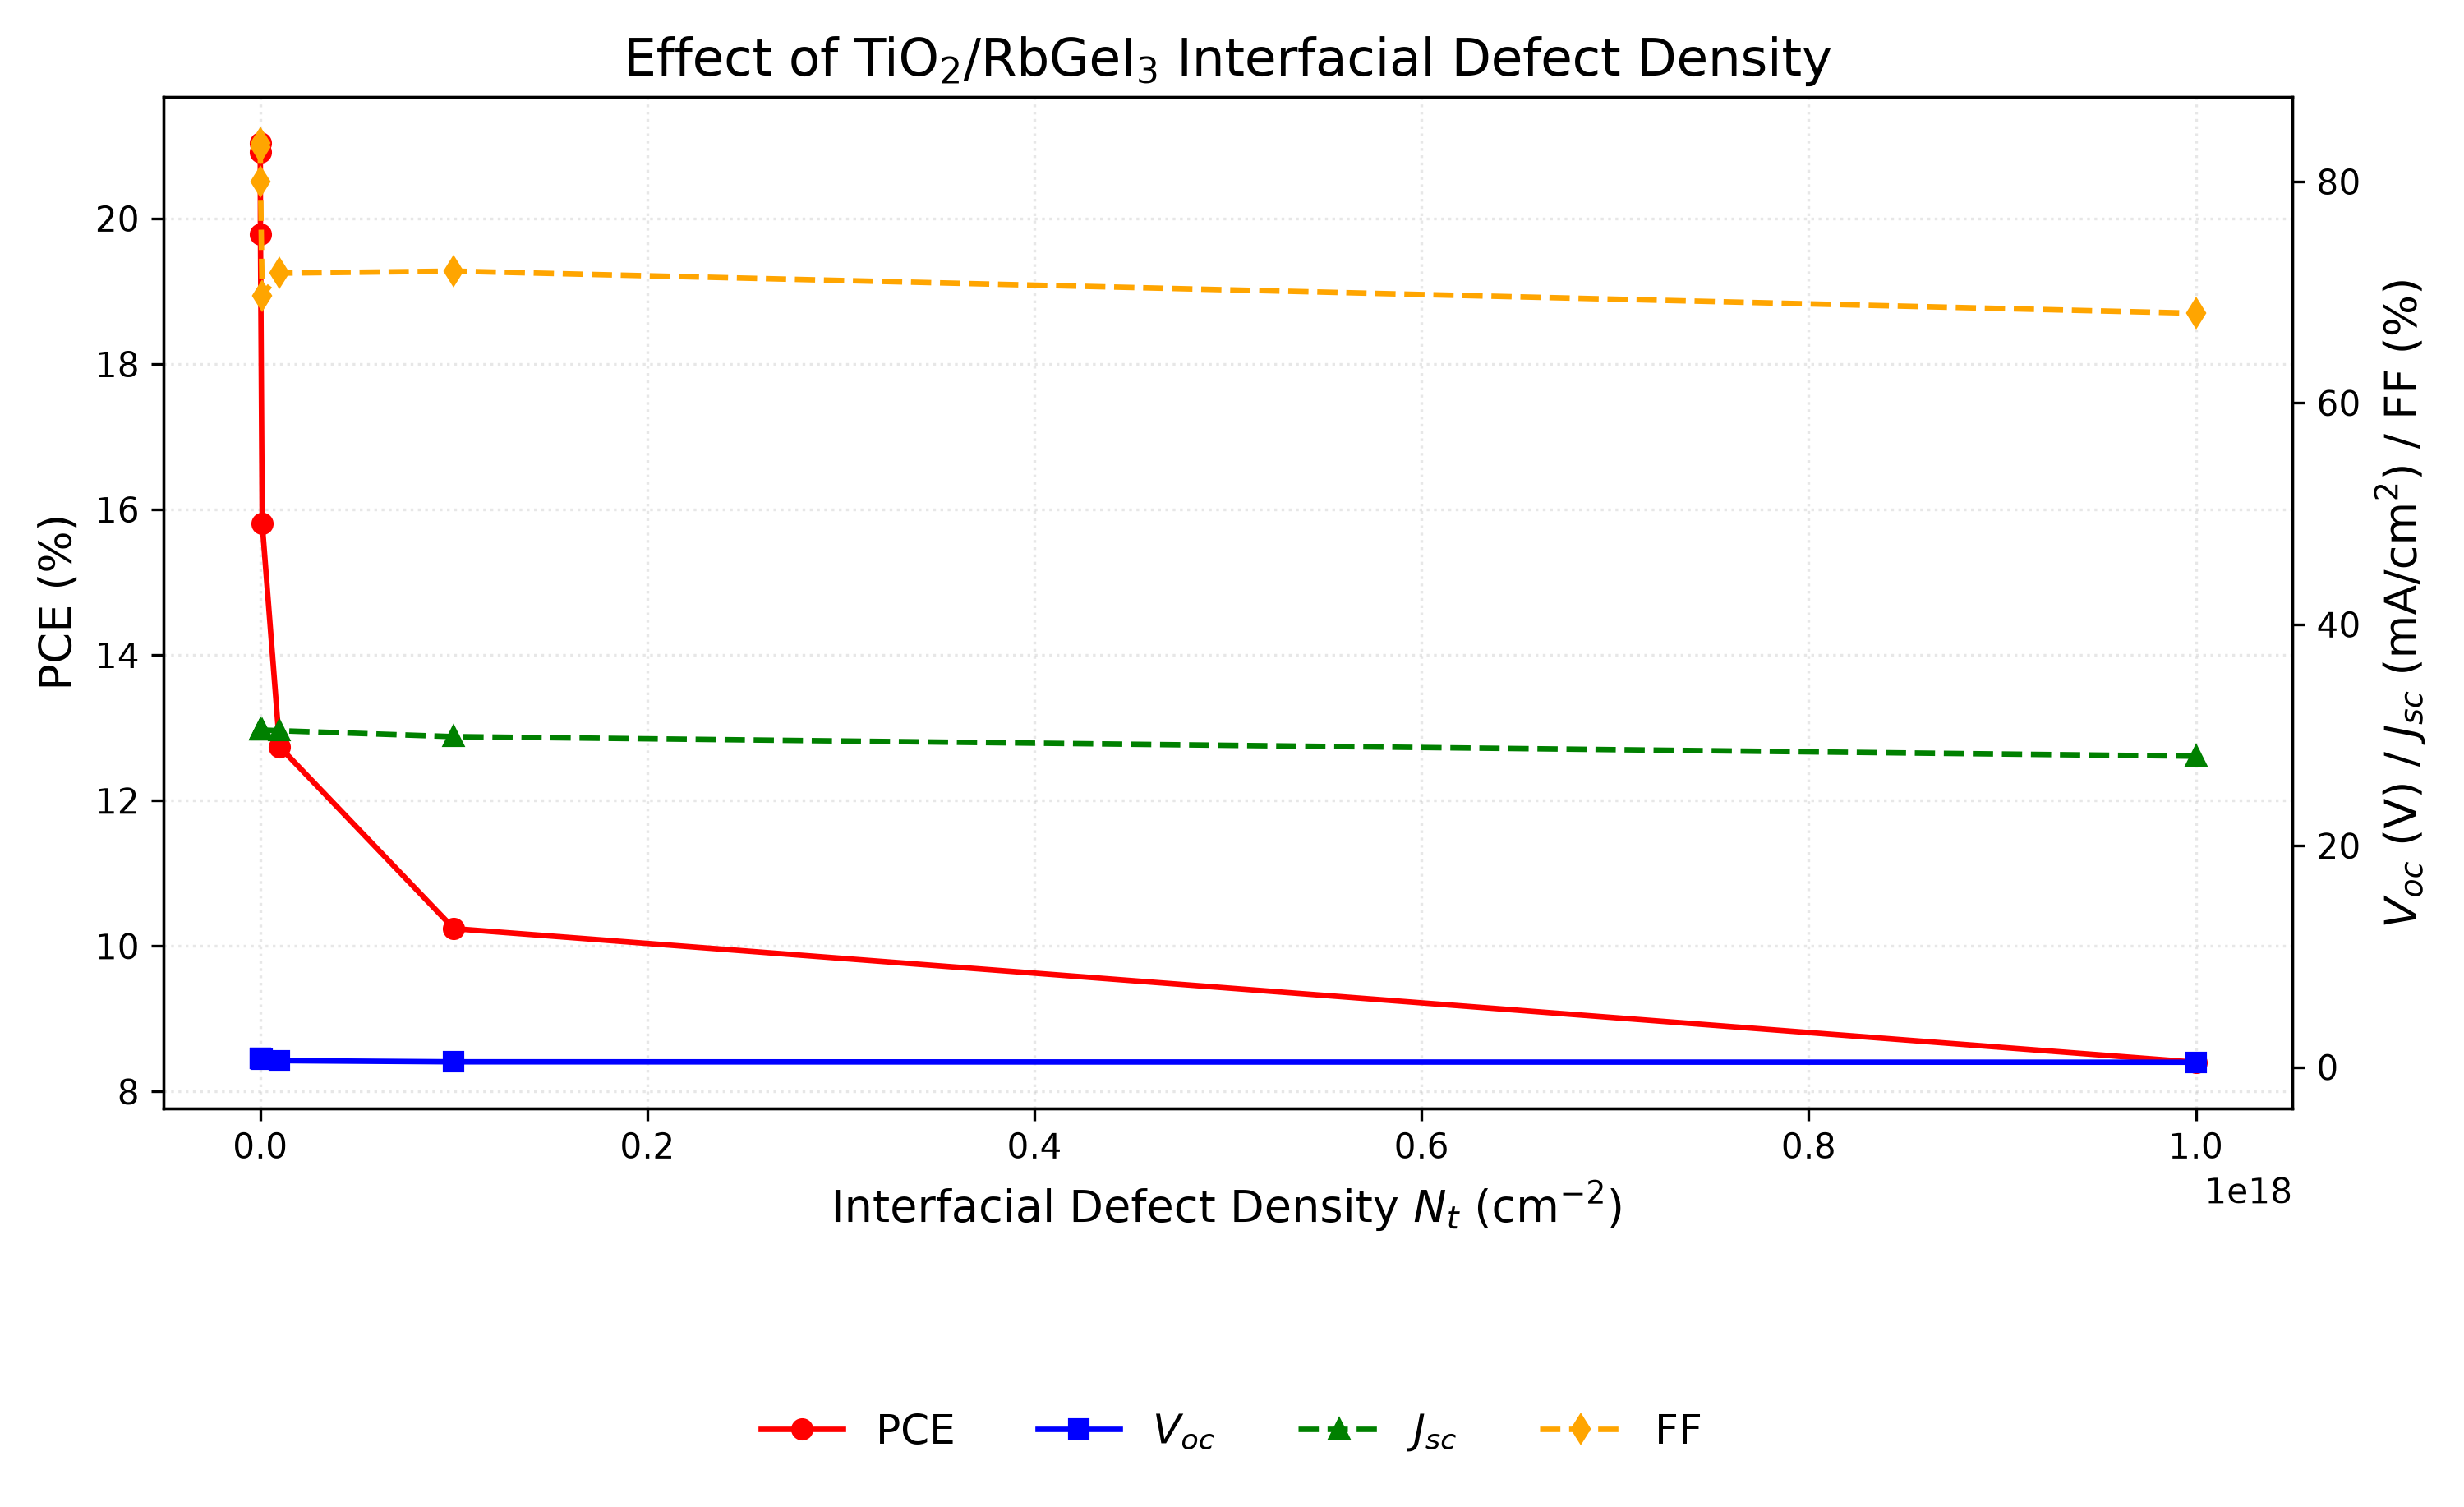
\includegraphics[width=0.85\linewidth]{figs/fig7.png}
\caption{Variation of PCE, V$_{\mathrm{OC}}$, J$_{\mathrm{SC}}$, and FF with TiO$_{2}$/RbGeI$_{3}$ interfacial defect density. Performance degrades sharply above 10$^{14}$ cm$^{-2}$; the RbGeI$_{3}$/CuI interface (Section V.G) is markedly more defect-tolerant.}
\end{figure}

\subsection{Effect of RbGeI$_{3}$/CuI interfacial defect density}
The RbGeI$_{3}$/CuI junction is far more tolerant: PCE moves only from 19.79\% to 18.19\% across the same 10$^{12}$ to 10$^{18}$ cm$^{-2}$ range. That contrast pins the performance limit on the TiO$_{2}$/RbGeI$_{3}$ interface. The final device still adopts 10$^{14}$ cm$^{-2}$ here to match the electron side (Section V.F); the modest penalty is the price of internal consistency.

\begin{figure}[htbp]
\centering
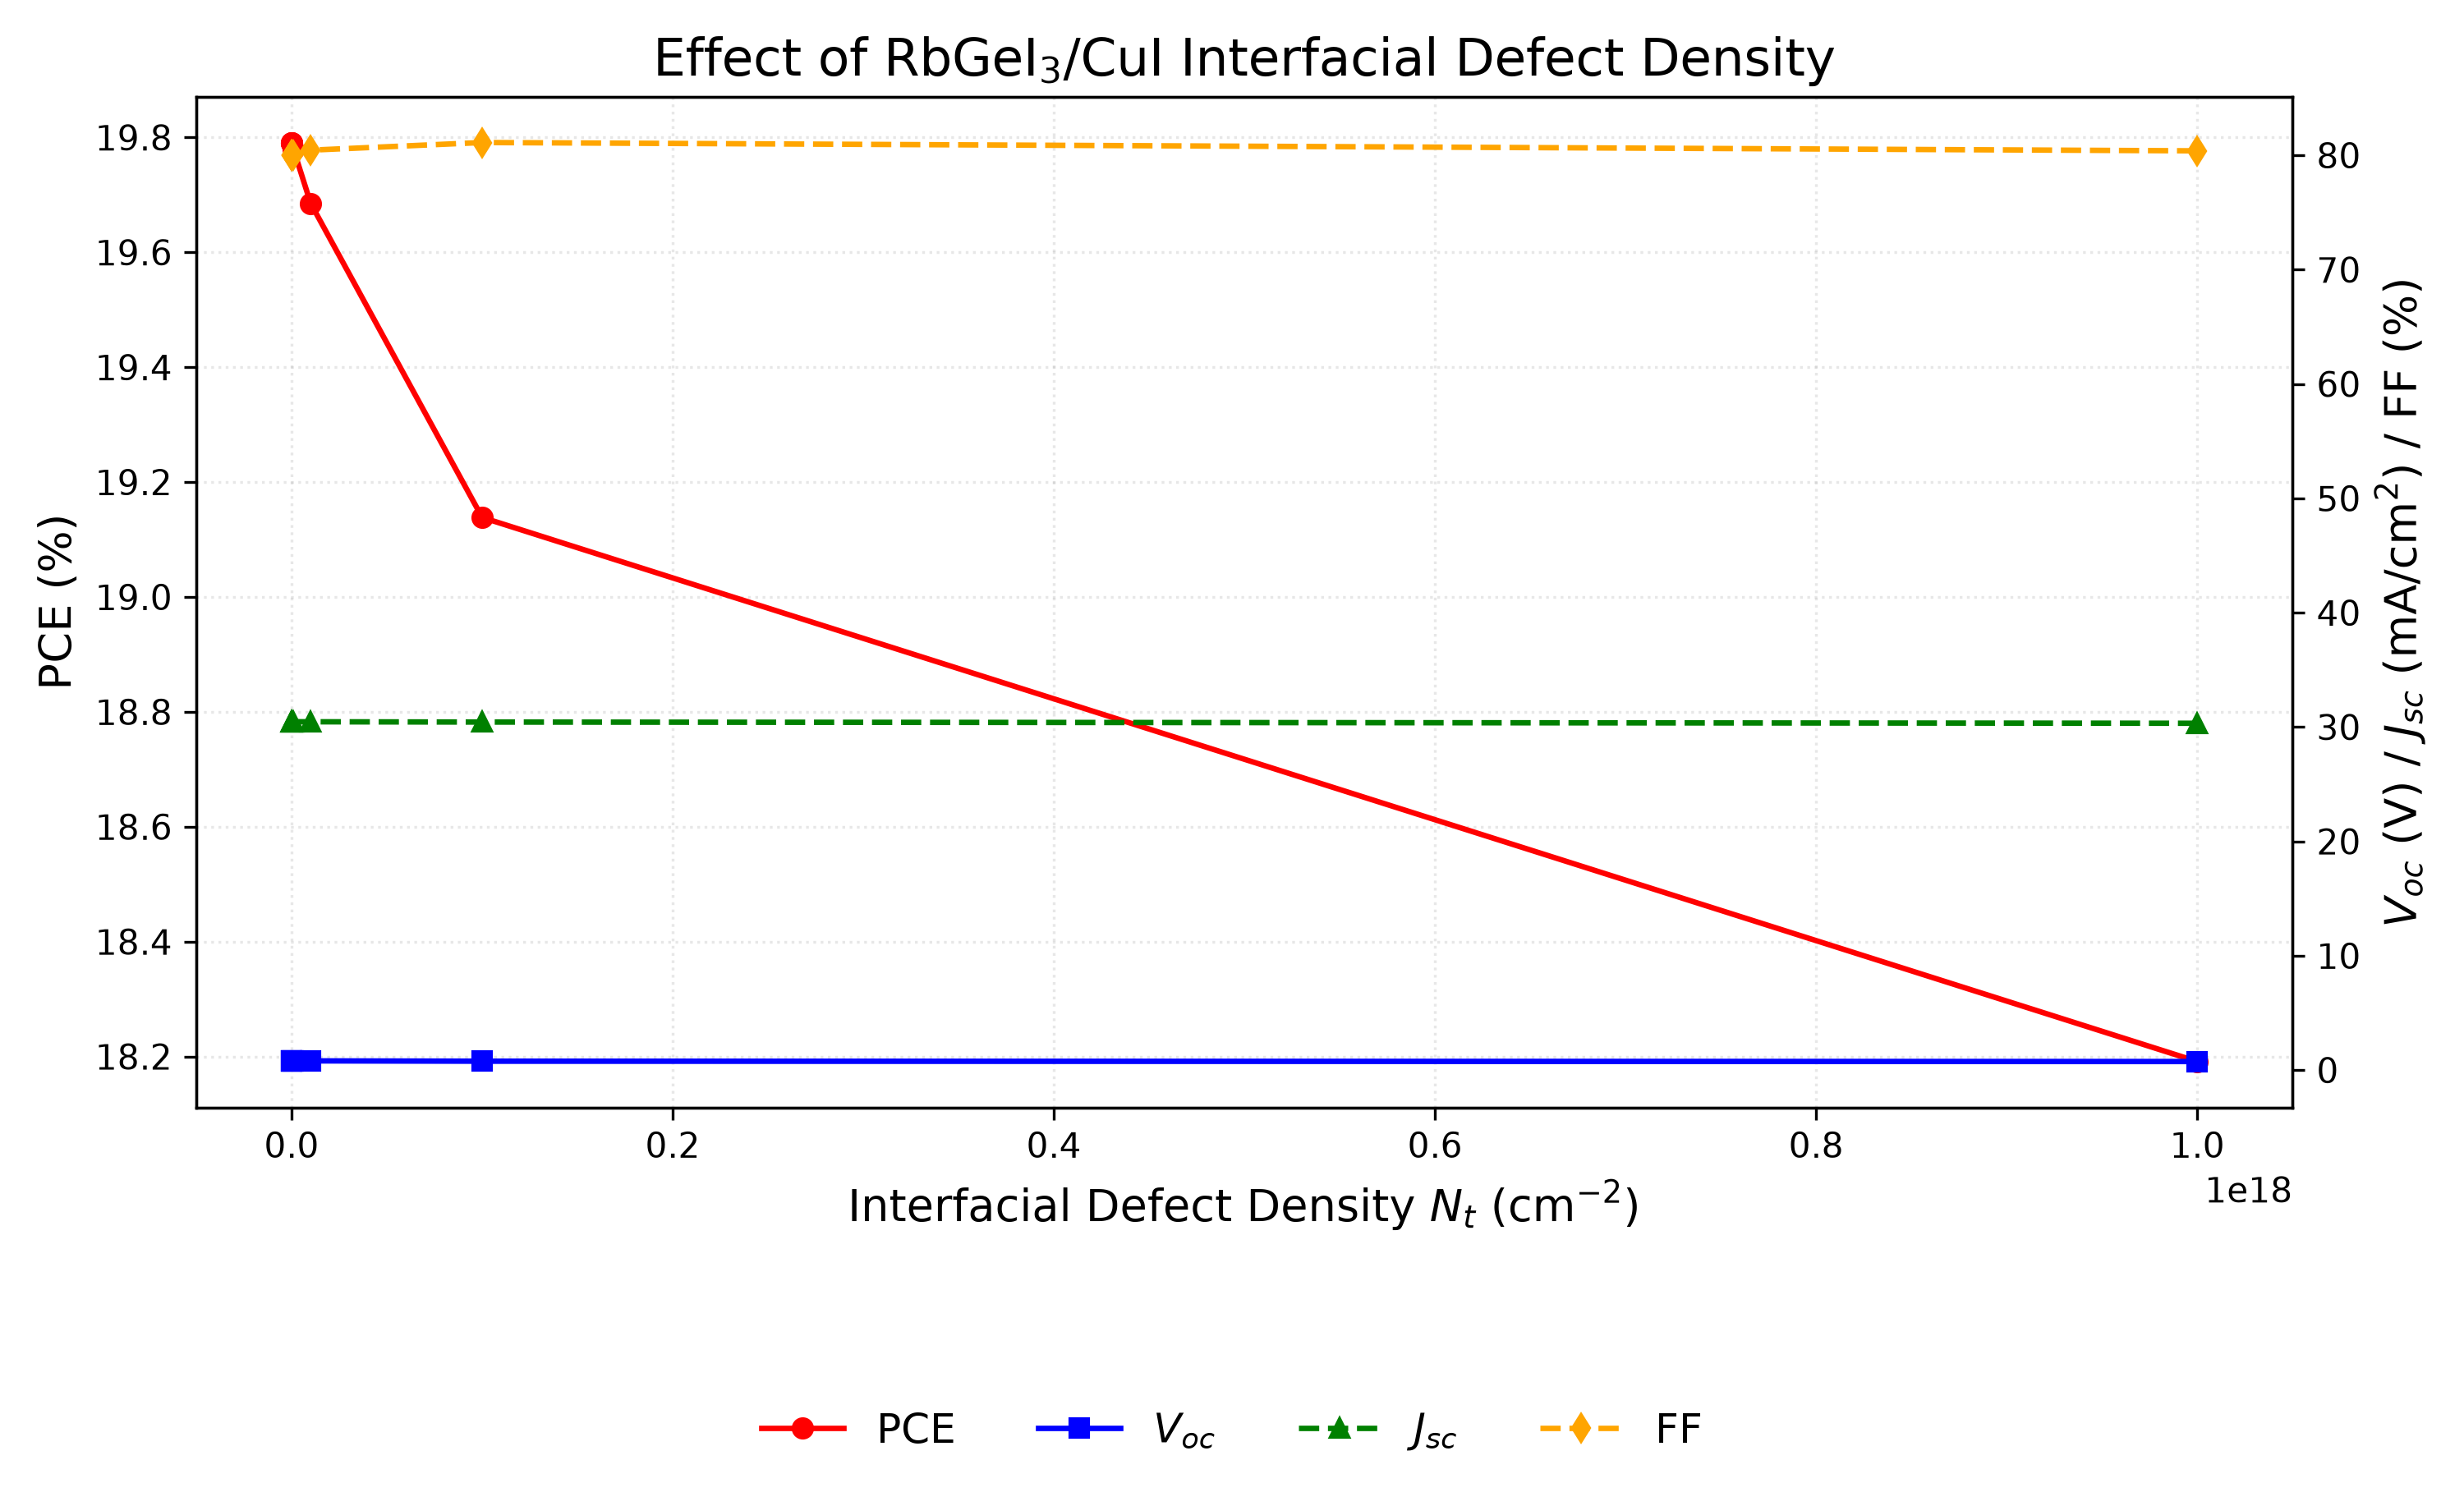
\includegraphics[width=0.85\linewidth]{figs/fig8.png}
\caption{Variation of PCE, V$_{\mathrm{OC}}$, J$_{\mathrm{SC}}$, and FF with RbGeI$_{3}$/CuI interfacial defect density. The interface is markedly more defect-tolerant than the TiO$_{2}$/RbGeI$_{3}$ interface; 10$^{14}$ cm$^{-2}$ is used here too.}
\end{figure}

\subsection{Effect of absorber bandgap}
The bandgap picks which wavelengths the cell can use. Moving it from 1.3 to 1.7 eV, all else constant, raises Voc from 0.840 V to 1.002 V as expected from larger quasi-Fermi-level splitting, while Jsc falls from 33.59 to 20.30 mA/cm$^{2}$ because a wider gap throws away more of the spectrum.
The maximum thus sits at 1.4 eV, within 0.06 eV of the Shockley--Queisser (SQ) optimum of $\approx$1.34 eV for a single junction \cite{r35,r36,r37}, so the absorber runs at 1.4 eV; tabulated SQ limits imply an ideal J$_{\mathrm{SC}}$ of $\approx$33 mA/cm$^{2}$ and a maximum efficiency of $\approx$33\% at this bandgap \cite{r36}. On both sides of the SQ optimum the limiting efficiency declines, steeply for wider bandgaps because fewer photons are absorbed \cite{r36,r37}: a 2.0 eV absorber would shift its absorption edge to $\lambda$c $\approx$ 620 nm and exclude most of the visible spectrum, and our sweep already shows J$_{\mathrm{SC}}$ falling to 20.30 mA/cm$^{2}$ at 1.7 eV, whereas at 1.3 eV the higher J$_{\mathrm{SC}}$ (33.59 mA/cm$^{2}$) does not offset the V$_{\mathrm{OC}}$ loss (0.840 V). The corresponding cutoff wavelength is $\lambda$c = 1240 / 1.4 $\approx$ 886 nm, consistent with the absorption edge observed in the quantum-efficiency spectrum of Section V.M. A targeted re-simulation varying only the absorption-grading endpoints (graded 885.7--1033.3 nm versus flat 885.7--885.7 nm, all else fixed) changes J$_{\mathrm{SC}}$ by 0.00 mA/cm$^{2}$, and the consolidated J$_{\mathrm{SC}}$ of 30.32 mA/cm$^{2}$ lies below the SQ limit of $\approx$33 mA/cm$^{2}$ at 1.4 eV, so the headline result is admissible with uniform square-root-law absorption at the electrical bandgap; the 26.81\% device is therefore reported as an ideal-coupling upper bound, with a quantified realistic window given in Sections V.P and VII.A.

\begin{figure}[htbp]
\centering
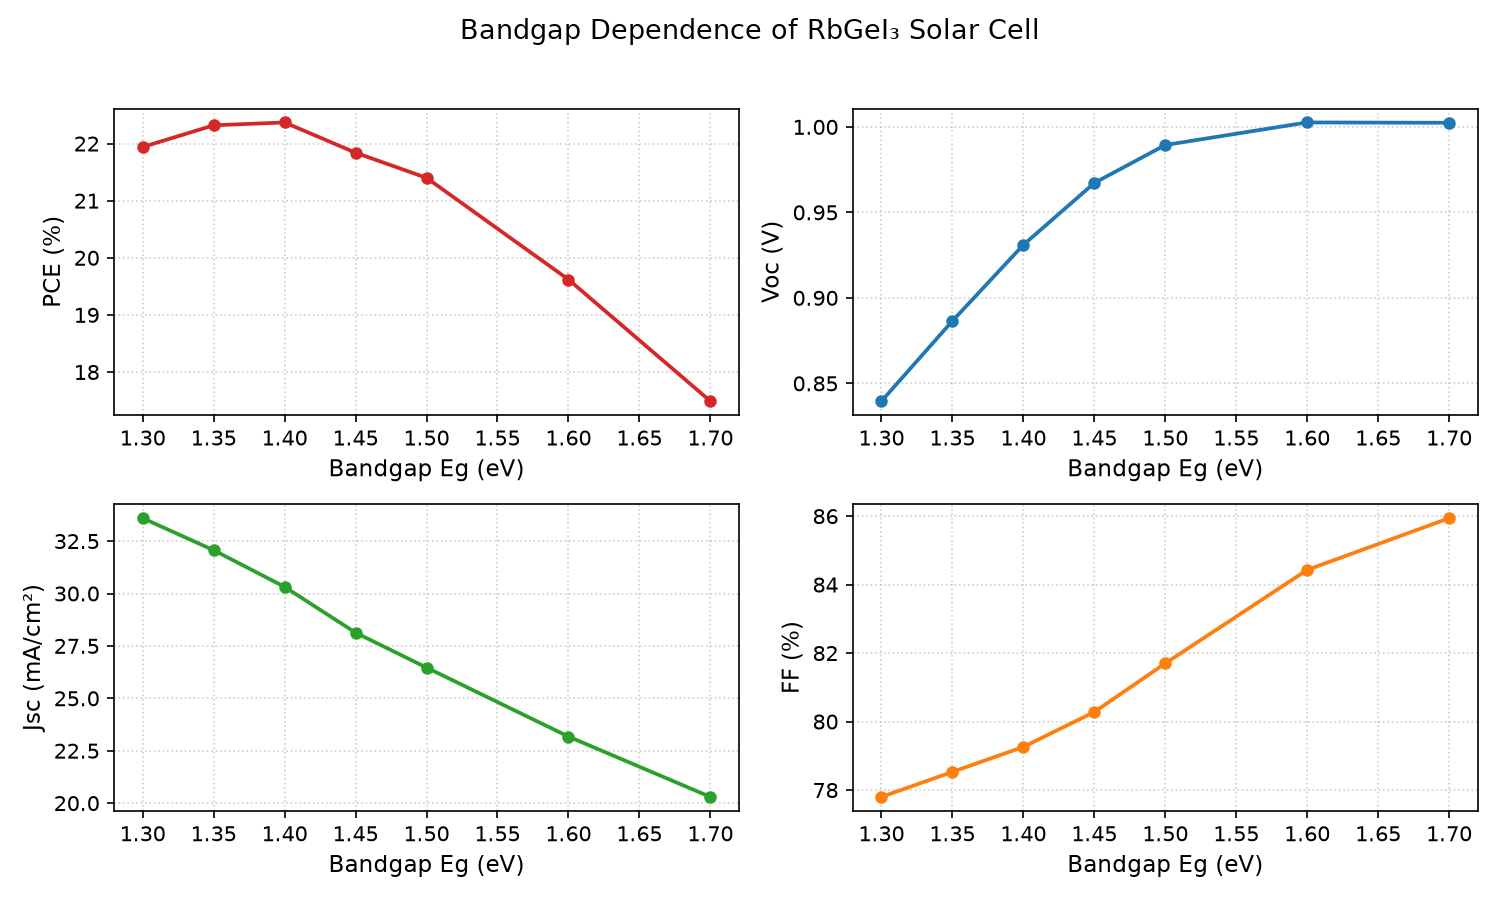
\includegraphics[width=0.85\linewidth]{figs/fig9.png}
\caption{Variation of PCE, V$_{\mathrm{OC}}$, J$_{\mathrm{SC}}$, and FF with RbGeI$_{3}$ absorber bandgap. PCE peaks at 1.4 eV, close to the Shockley--Queisser optimum.}
\end{figure}

\subsection{Effect of TiO$_{2}$ ETL thickness}
Thickness of the TiO$_{2}$ ETL cuts across electron extraction, transport, and optical transmission at once. Sweeping it from 0.01 to 0.09 $\mu$m, all else fixed, gives the best PCE at the thinnest layers: 21.12\% at 10 nm, a local low of 18.72\% at 0.04 $\mu$m, and a partial recovery to 19.97\% at 0.09 $\mu$m. Planar SCAPS studies stick to thin ($\leq$50 nm) ETLs for the same reason we do: thicker ones add series resistance and soak up photons.

\begin{figure}[htbp]
\centering
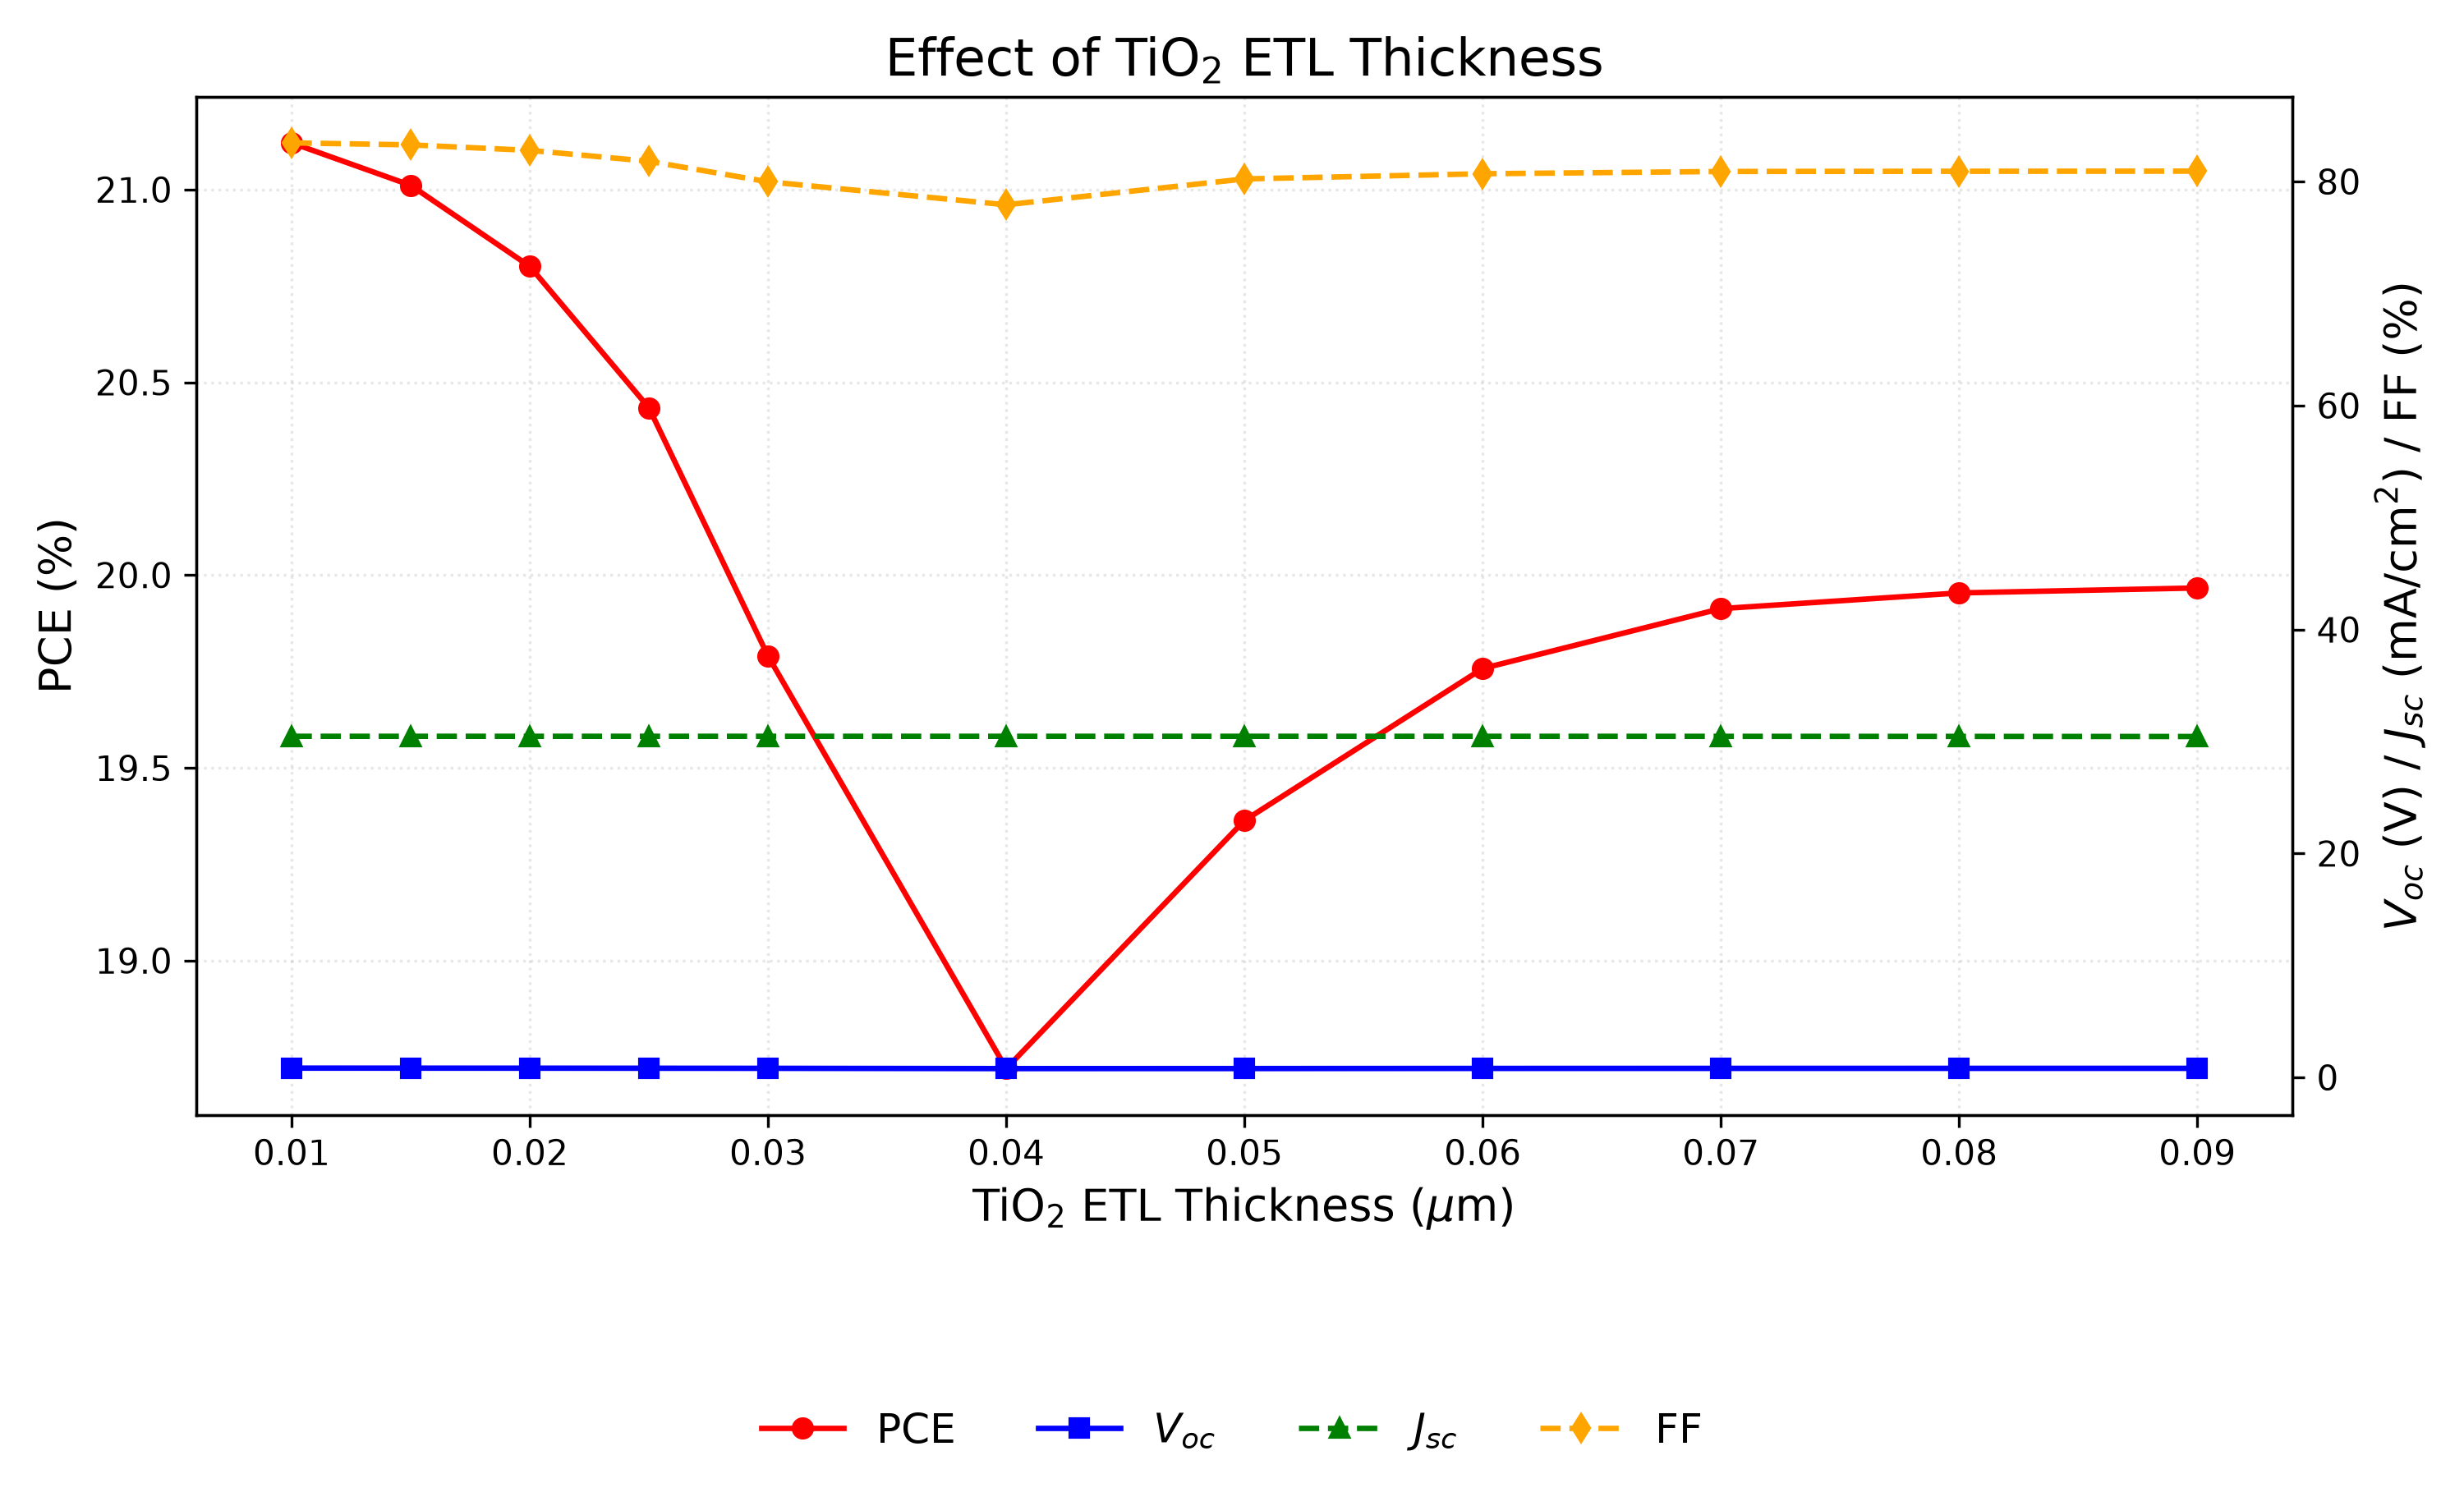
\includegraphics[width=0.85\linewidth]{figs/fig10.png}
\caption{Variation of PCE, V$_{\mathrm{OC}}$, J$_{\mathrm{SC}}$, and FF with TiO$_{2}$ ETL thickness. PCE is highest at the thinnest ETL (10 nm), reflecting the shorter electron transport path.}
\end{figure}

\subsection{Effect of CuI HTL thickness}
CuI thickness, swept from 0.1 to 1.9 $\mu$m, moves PCE by less than 0.002 percentage points; V$_{\mathrm{OC}}$, J$_{\mathrm{SC}}$, and FF stay essentially constant. That flatness lets us pick 100 nm purely to minimize material use. It sits at the low end of the 0.1--1.0 $\mu$m range comparable studies explored, which also reported a weak dependence.

\begin{figure}[htbp]
\centering
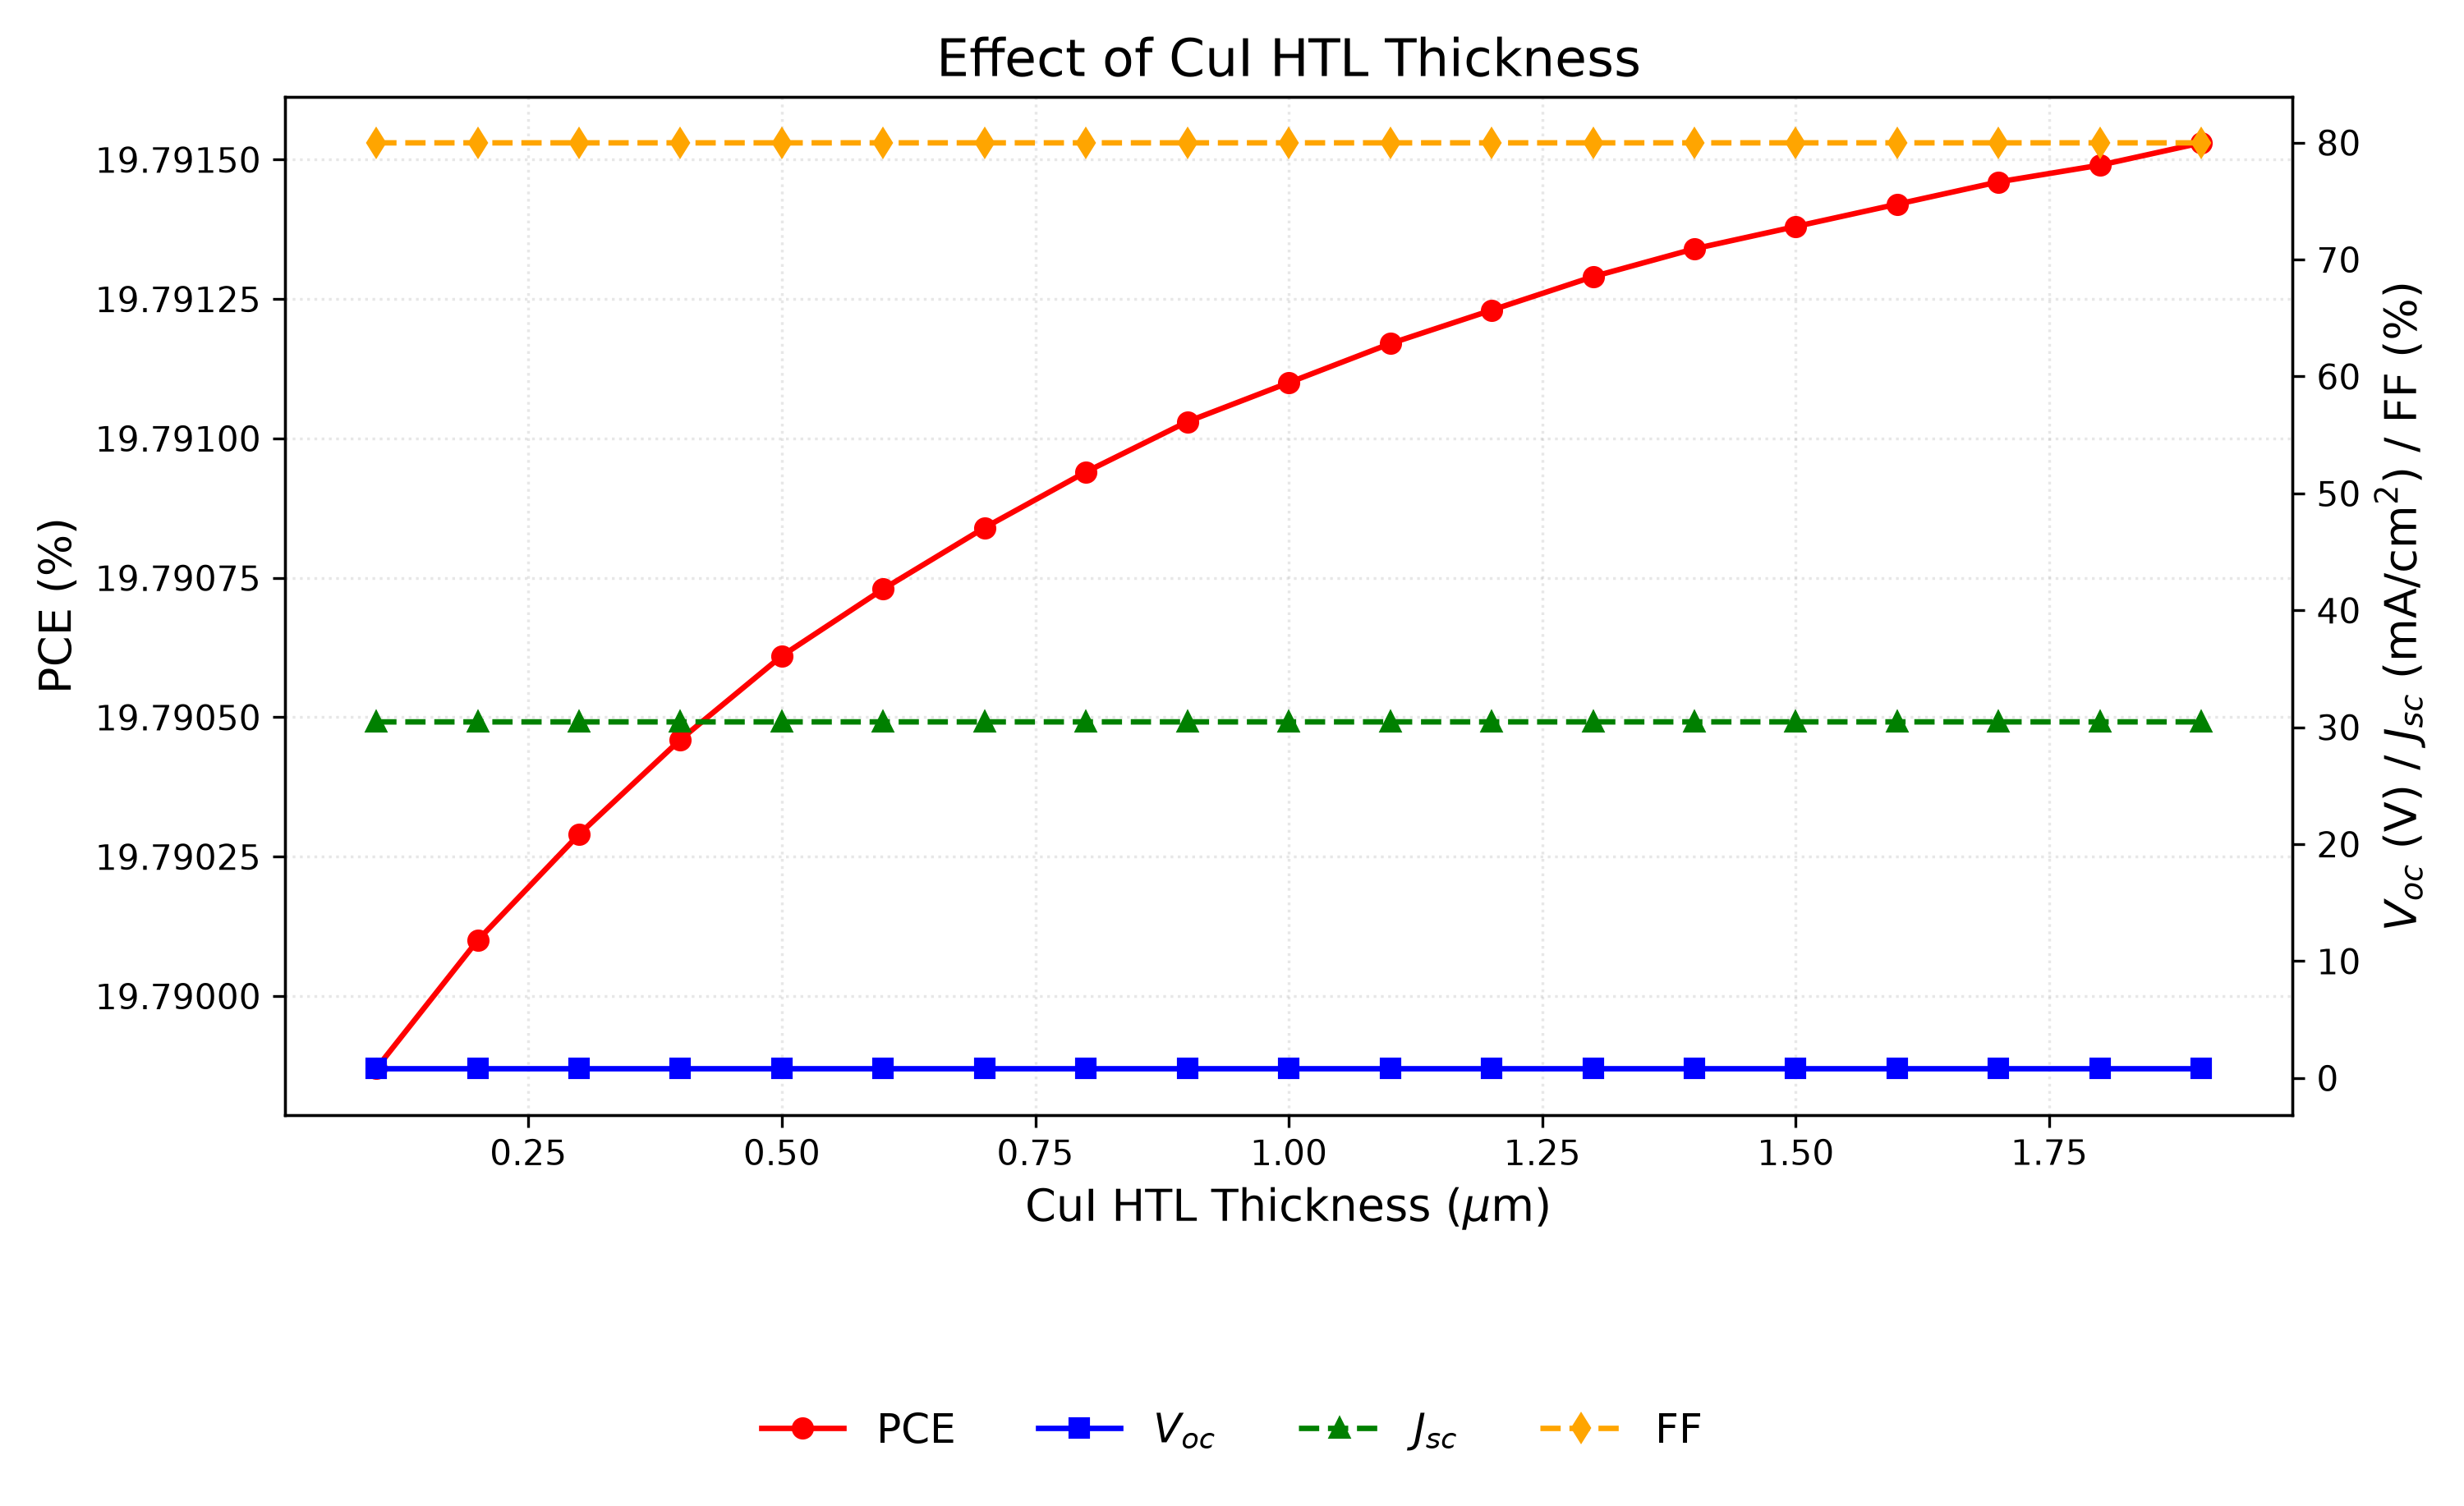
\includegraphics[width=0.85\linewidth]{figs/fig11.png}
\caption{Variation of PCE, V$_{\mathrm{OC}}$, J$_{\mathrm{SC}}$, and FF with CuI HTL thickness. The performance is essentially independent of HTL thickness; 100 nm minimizes material usage.}
\end{figure}

\subsection{Effect of conduction-band effective density of states N$_{\mathrm{C}}$}
Raising N$_{\mathrm{C}}$ from 1$\times$10$^{17}$ to 1$\times$10$^{20}$ cm$^{-3}$ pushes PCE monotonically down from 20.65\% to 18.15\%; V$_{\mathrm{OC}}$ carries the loss (0.859 to 0.764 V) while J$_{\mathrm{SC}}$ barely stirs at $\sim$30.46 mA/cm$^{2}$. A lower N$_{\mathrm{C}}$ means a lower intrinsic carrier density and therefore a higher V$_{\mathrm{OC}}$, so the bottom of the sweep, 1$\times$10$^{17}$ cm$^{-3}$, goes into the final device. SCAPS studies commonly assume $\approx$10$^{18}$ cm$^{-3}$ for lead-free absorbers; we find going lower helps.

\begin{figure}[htbp]
\centering
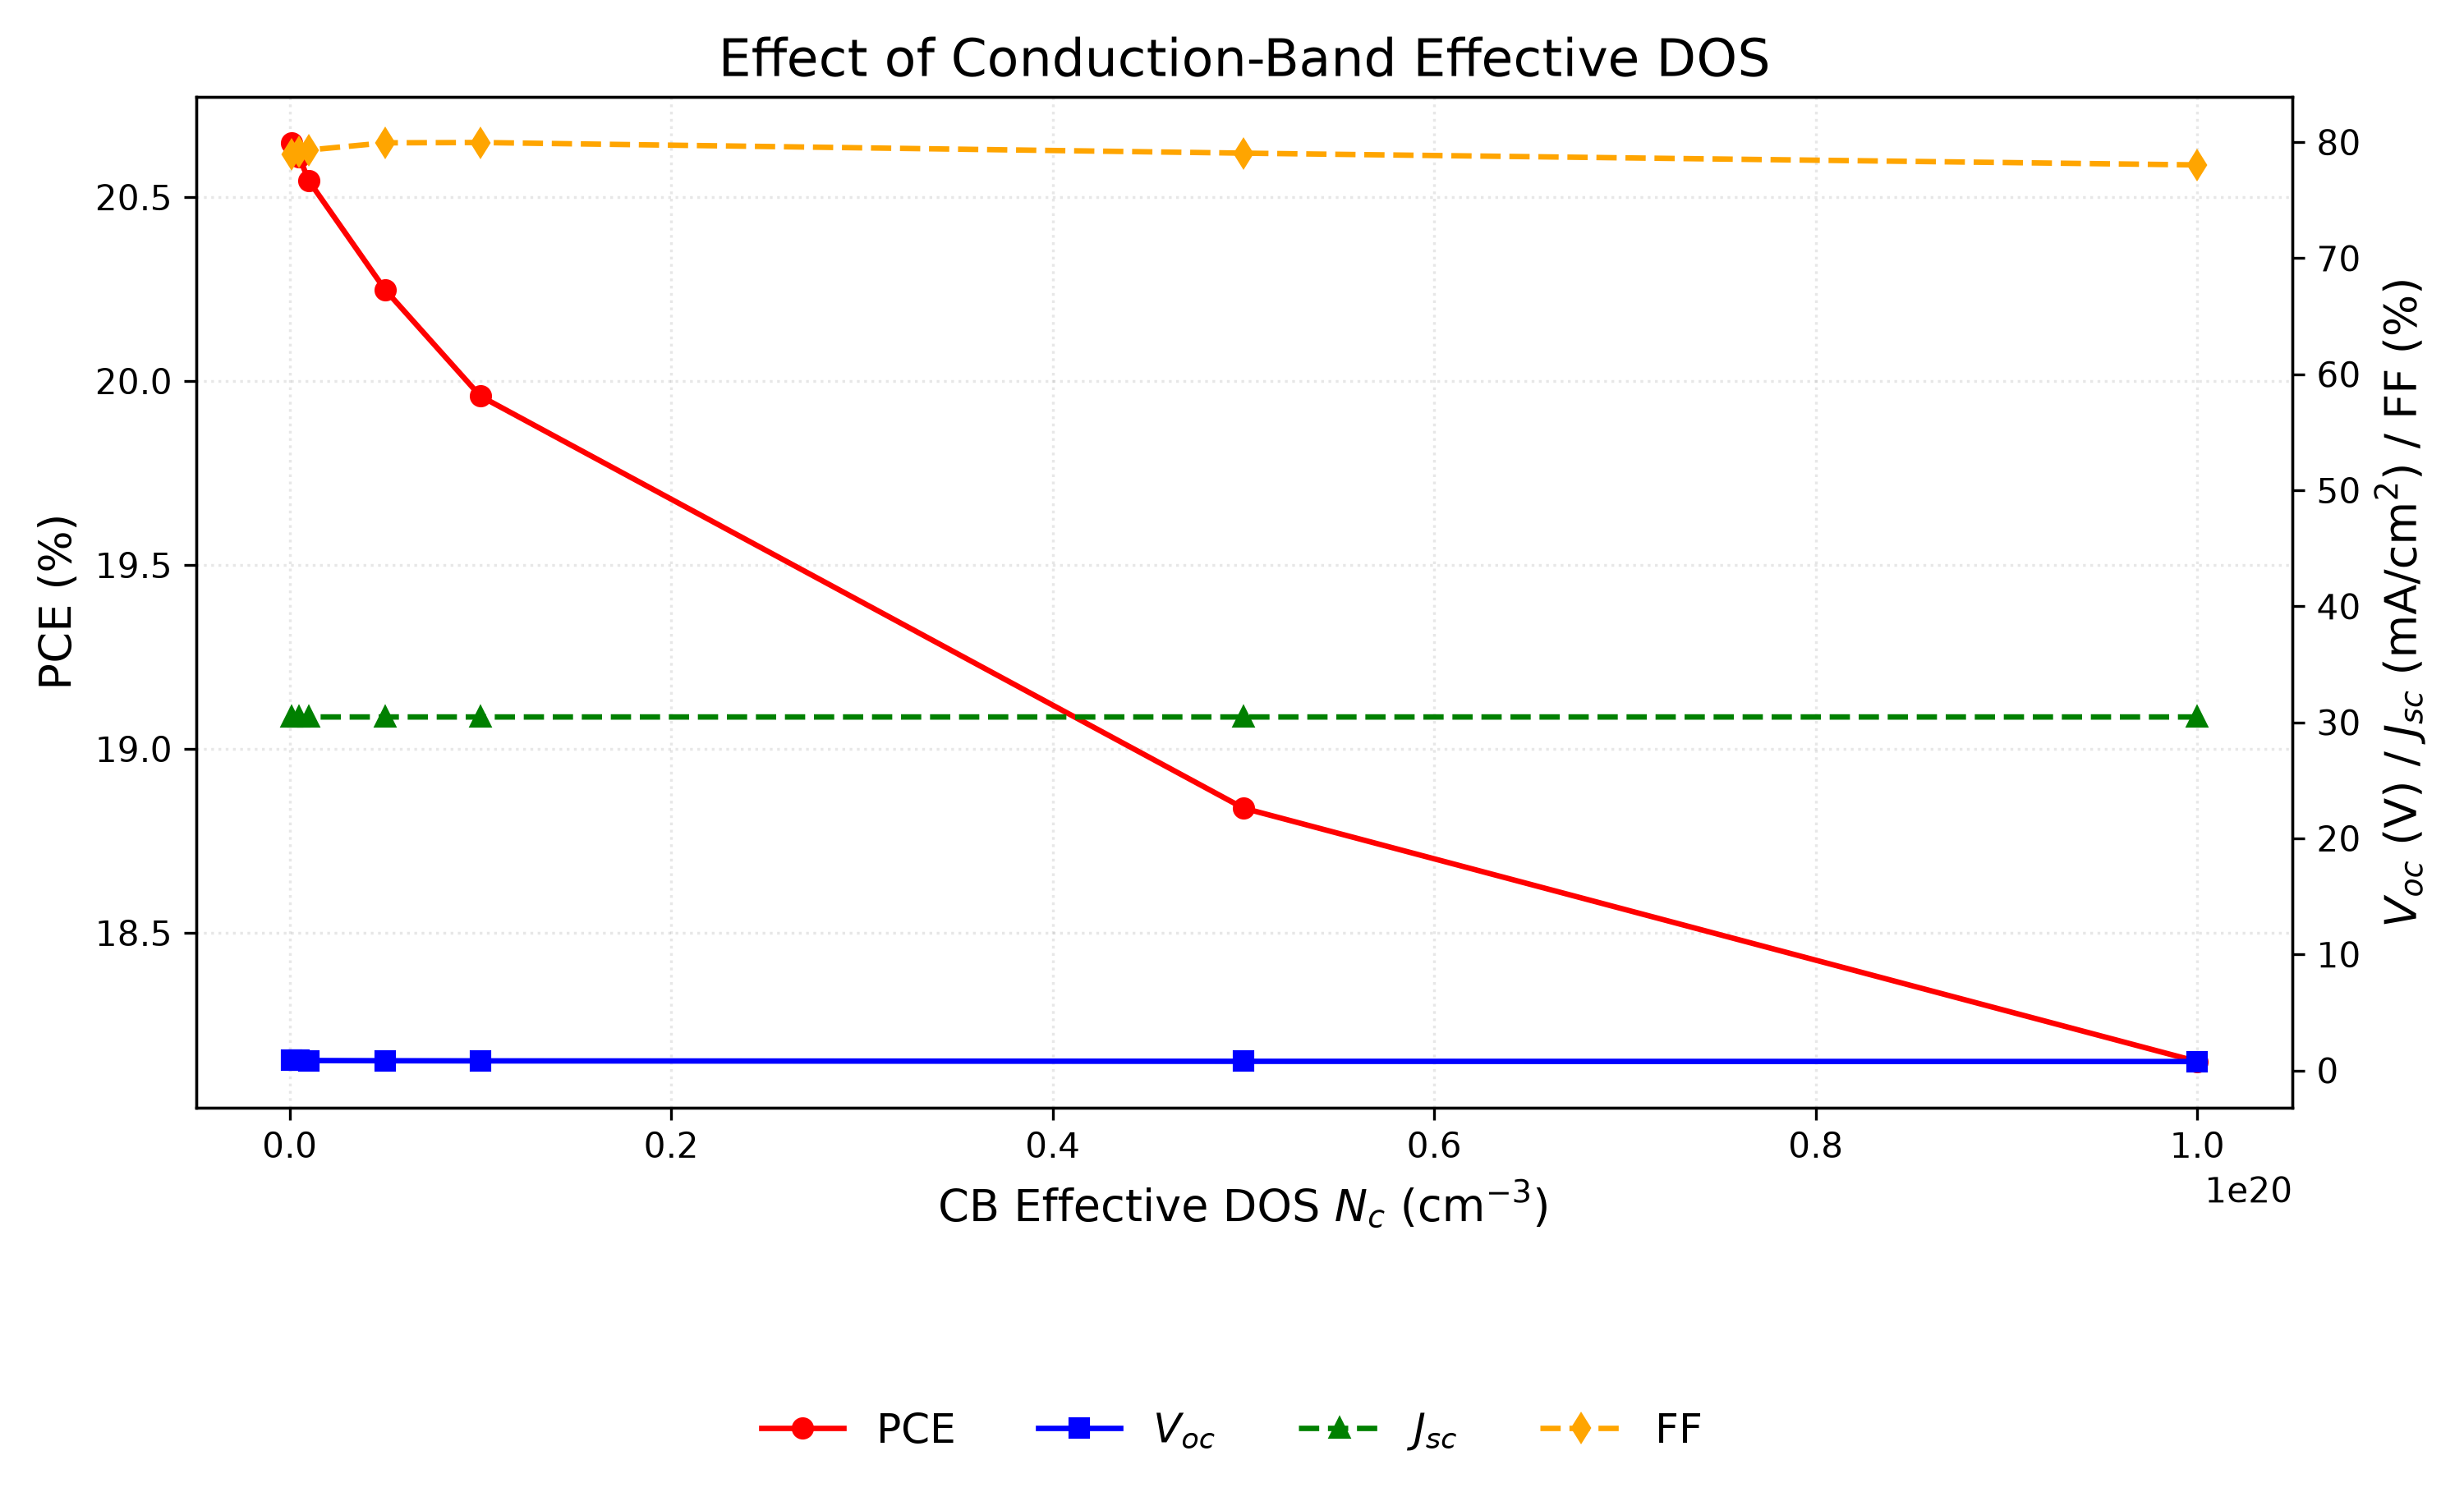
\includegraphics[width=0.85\linewidth]{figs/fig12.png}
\caption{Variation of PCE, V$_{\mathrm{OC}}$, J$_{\mathrm{SC}}$, and FF with conduction-band effective density of states N$_{\mathrm{C}}$. Lower N$_{\mathrm{C}}$ is preferred; the best value is 10$^{17}$ cm$^{-3}$.}
\end{figure}

\subsection{Effect of valence-band effective density of states N$_{\mathrm{V}}$}
N$_{\mathrm{V}}$ behaves like N$_{\mathrm{C}}$ but hits harder. Across 1$\times$10$^{17}$ to 1$\times$10$^{20}$ cm$^{-3}$, PCE drops from 23.54\% to 18.86\% as V$_{\mathrm{OC}}$ slides from 0.945 to 0.780 V with J$_{\mathrm{SC}}$ flat. The smallest value wins again: N$_{\mathrm{V}}$ = 1$\times$10$^{17}$ cm$^{-3}$ is carried into the final set.

\begin{figure}[htbp]
\centering
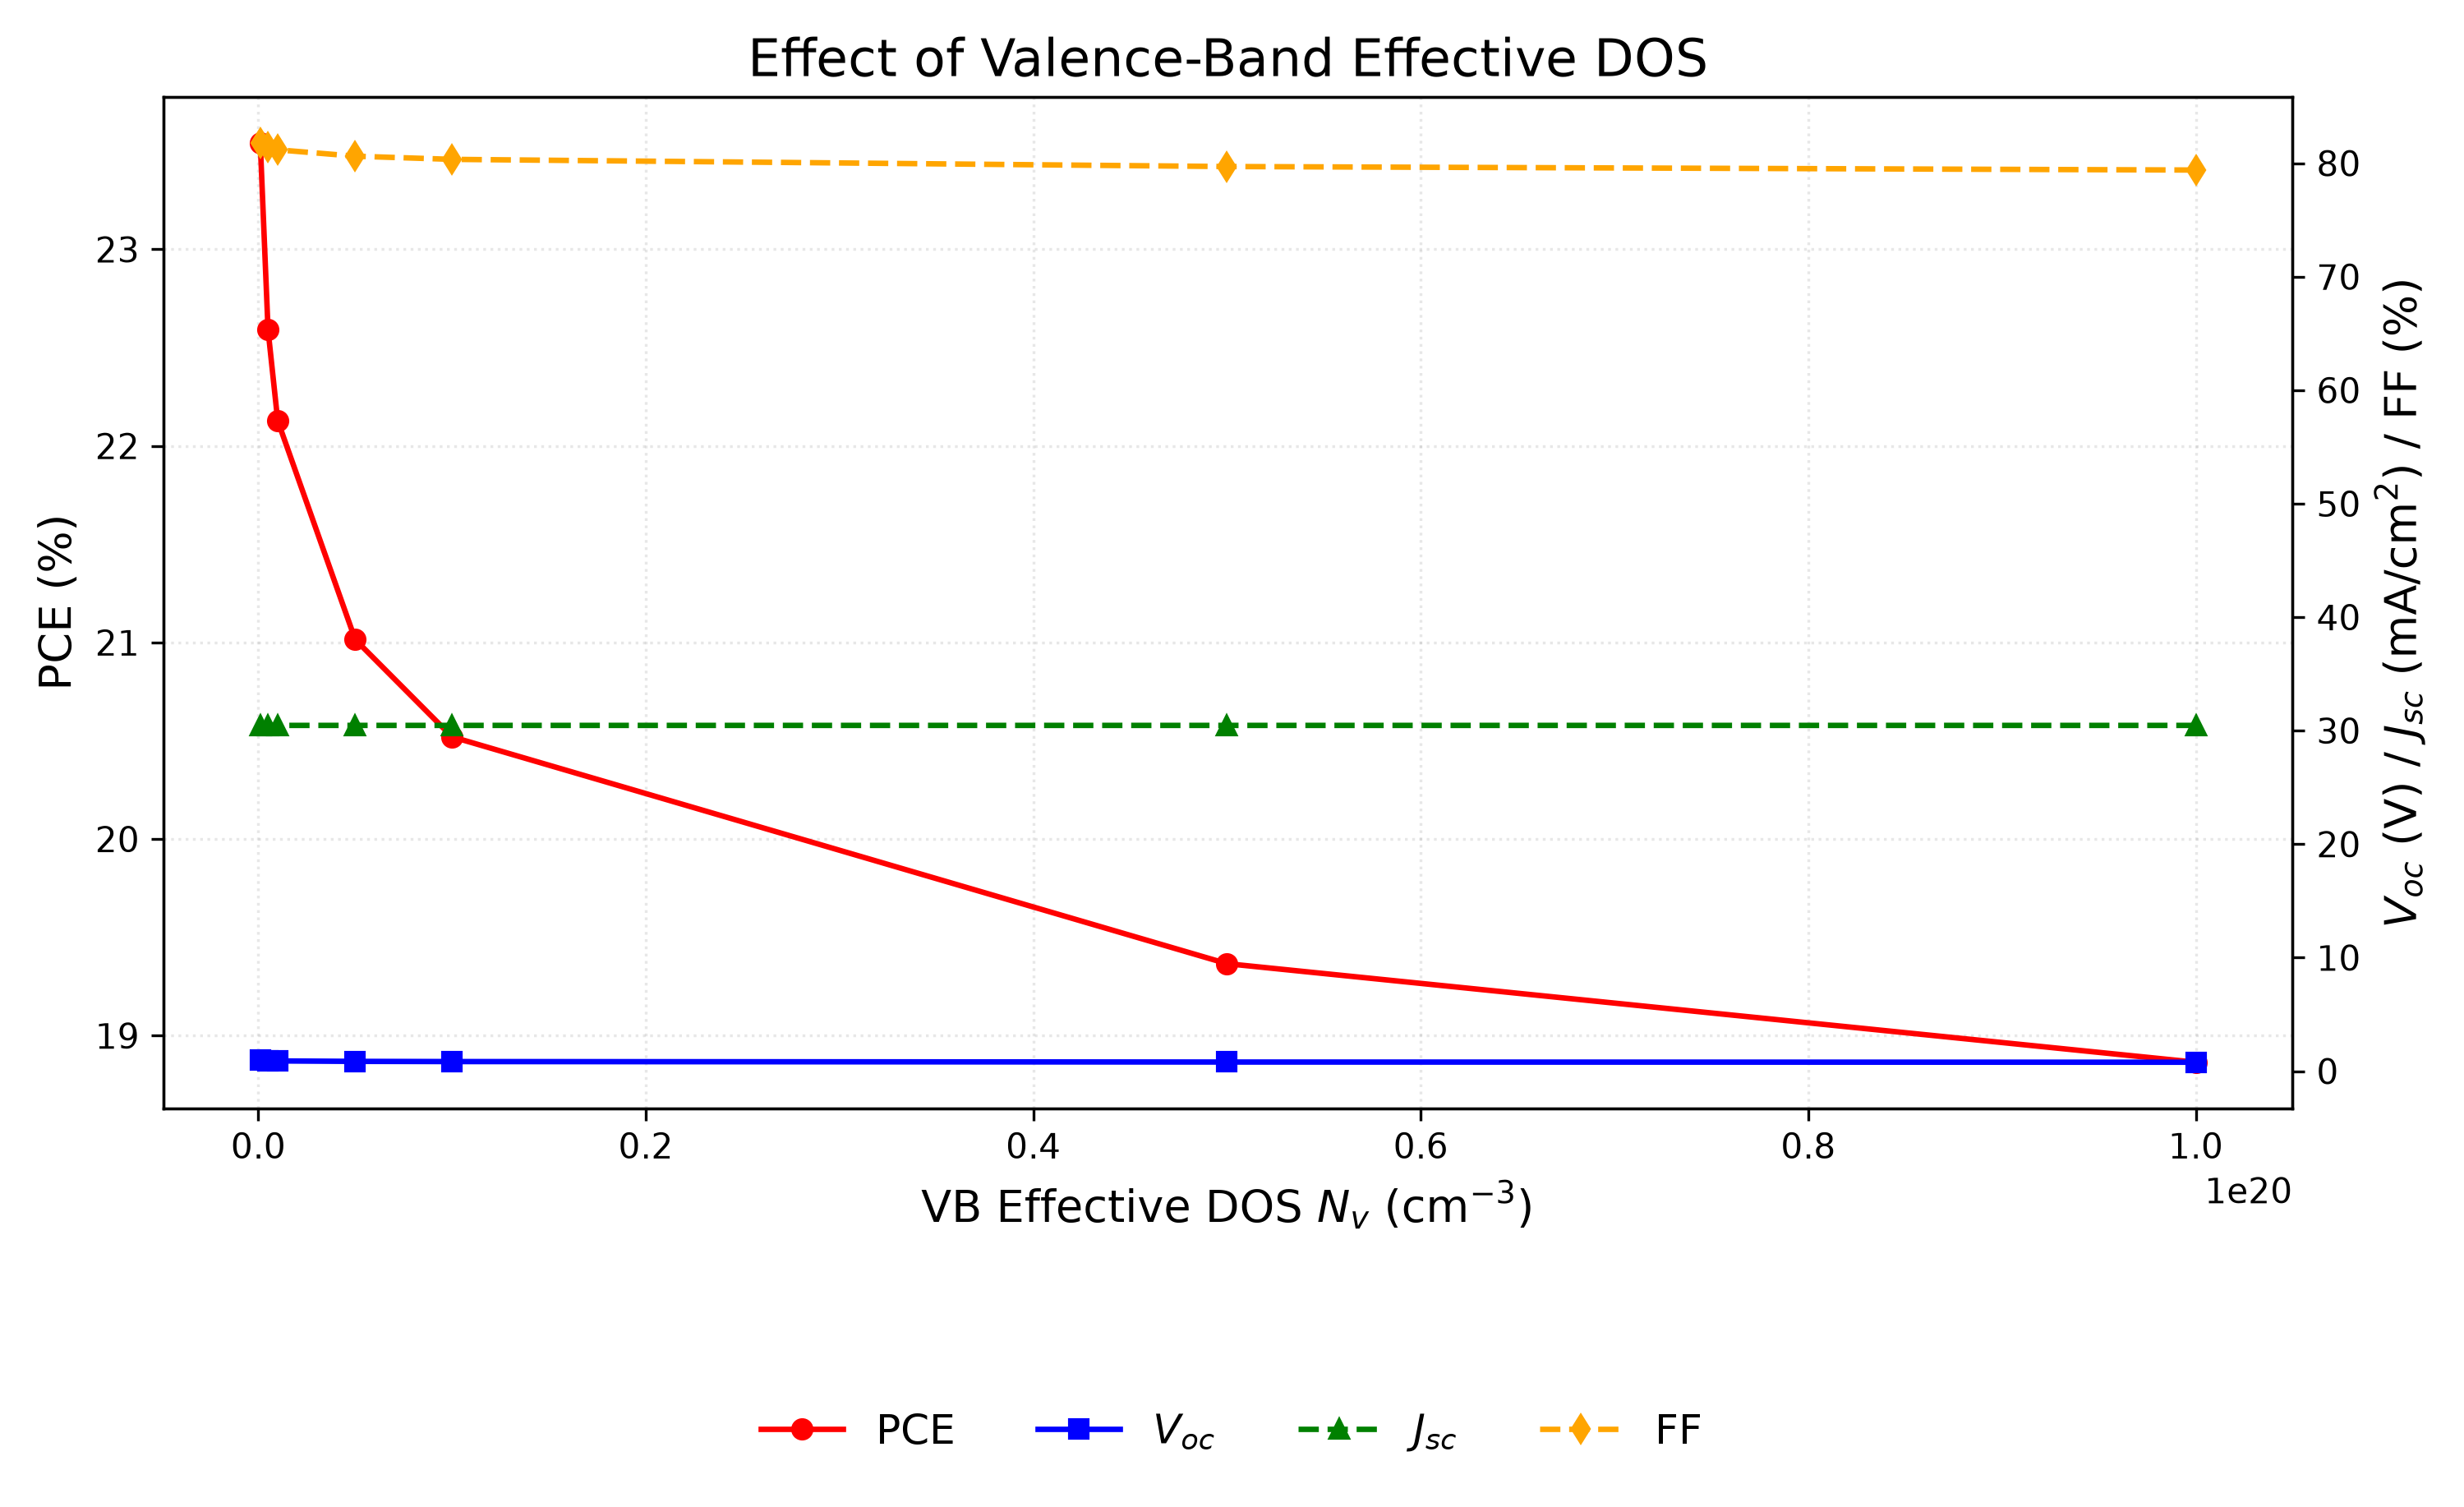
\includegraphics[width=0.85\linewidth]{figs/fig13.png}
\caption{Variation of PCE, V$_{\mathrm{OC}}$, J$_{\mathrm{SC}}$, and FF with valence-band effective density of states N$_{\mathrm{V}}$. The effect is more pronounced than for N$_{\mathrm{C}}$; the best value is 10$^{17}$ cm$^{-3}$.}
\end{figure}

\subsection{Quantum efficiency analysis}
Figure 14 tracks the quantum efficiency of the optimized cell, that is, how many collected carriers each incident photon yields. QE climbs from 34.52\% at 300 nm to 49.18\% at 350 nm and levels out near 100\% at 400 nm. The suppressed ultraviolet response is surface recombination: high-energy photons are absorbed so close to the front that some carriers die before collection \cite{r21,r38}.
Absorption in the visible is excellent: QE holds near 100\% from 400 to 650 nm, then eases to 76\% at 850 nm and cuts off near 900 nm, matching the 1.4 eV gap ($\lambda$c $\approx$ 886 nm). Integrating the spectrum gives $\approx$23.3 mA/cm$^{2}$, short of the 30.32 mA/cm$^{2}$ read from the J--V curve. The integral shortfall is a deck-version difference, not physics: the QE spectrum was archived from the earlier sweep-campaign deck (the same deck generation that produced the the Section V.B sweep record offset discussed in Section V.H), whereas the J--V metrics come from the consolidated deck. Re-simulation with the consolidated deck gives identical J--V with flat or graded absorption endpoints ($\Delta$JSC = 0.00 mA/cm$^{2}$), so no absorption-model difference can account for the gap. The QE curve is therefore retained only for its edge shape ($\lambda$c $\approx$ 886 nm, consistent with 1.4 eV); the J--V-derived J$_{\mathrm{SC}}$ = 30.32 mA/cm$^{2}$ is the reported metric.

\begin{figure}[htbp]
\centering
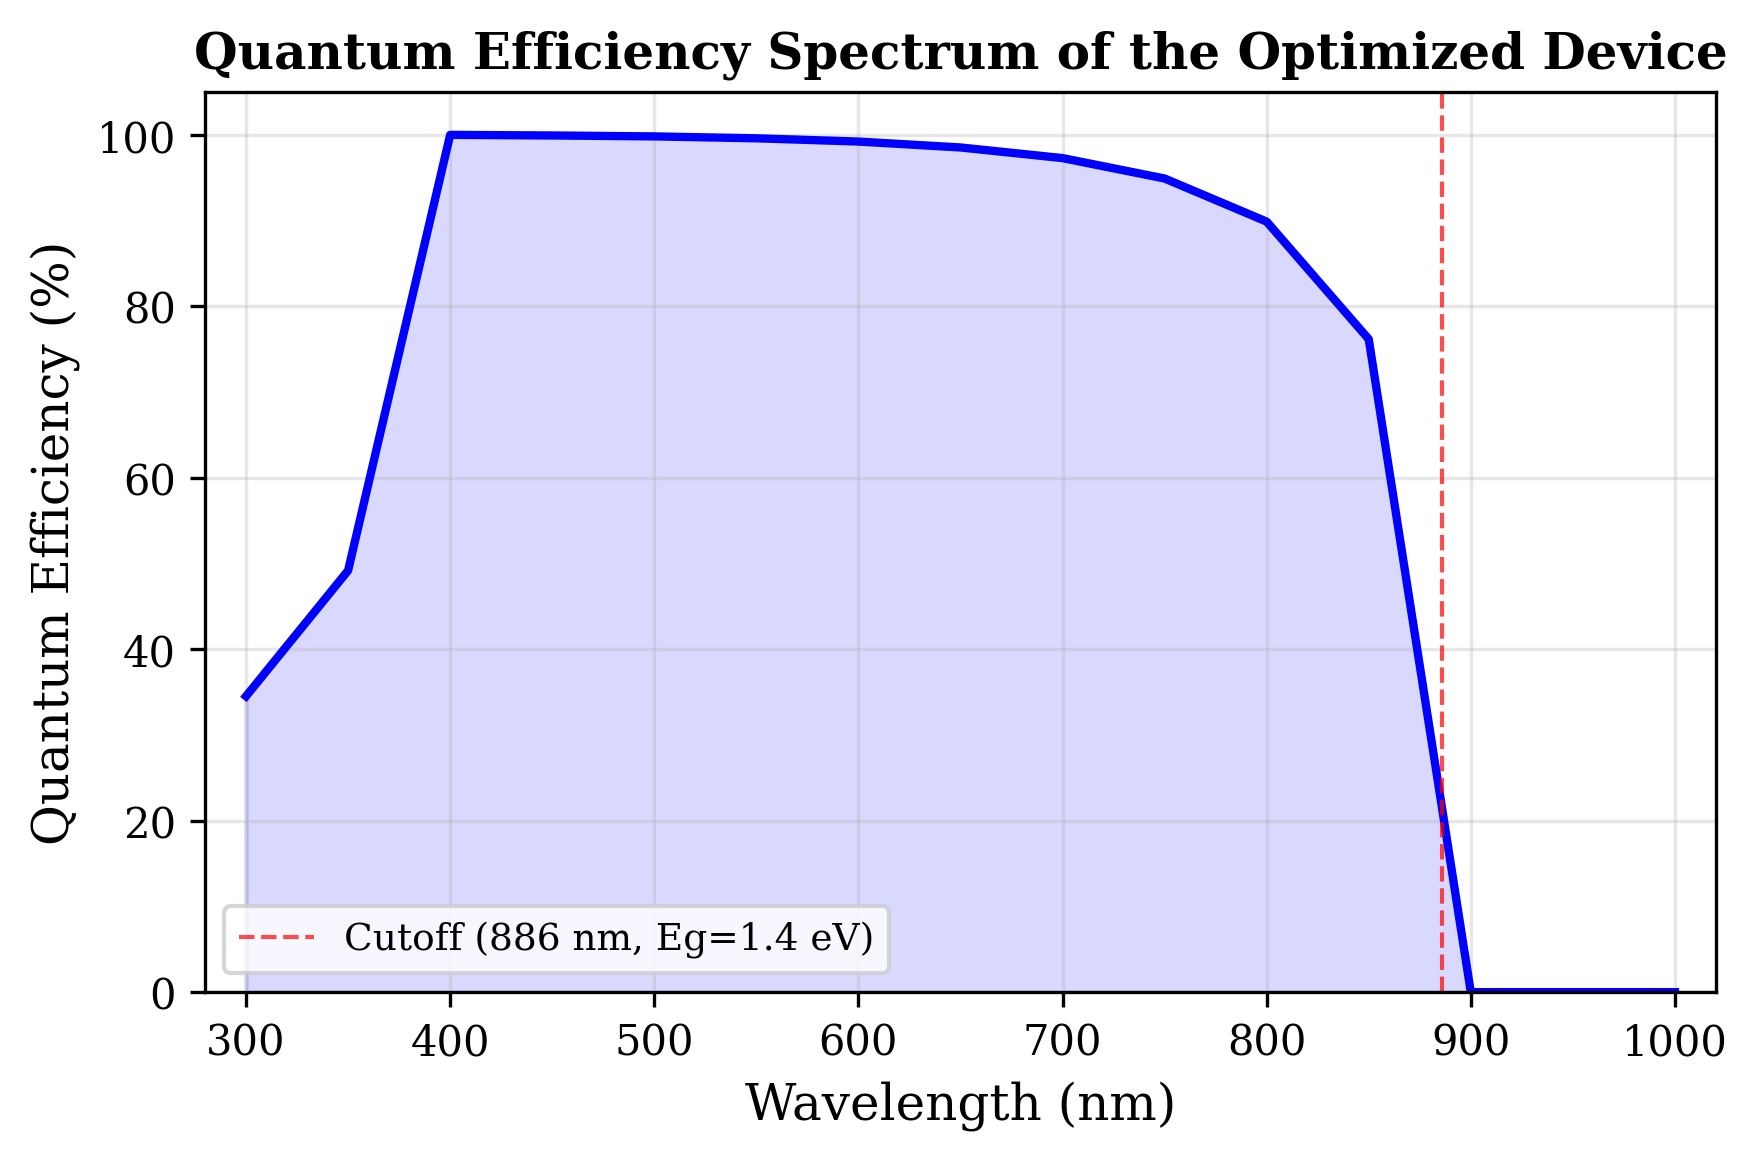
\includegraphics[width=0.85\linewidth]{figs/fig14.png}
\caption{Variation of quantum efficiency (QE) with incident wavelength of the optimized solar cell. The cutoff at $\approx$886 nm corresponds to the absorber bandgap of 1.4 eV.}
\end{figure}

\subsection{Energy band diagram analysis}
The energy band diagram of the optimized device under illumination (Figure 15) shows the energy alignment across the device: the 1.8 eV conduction-band offset at CuI/\allowbreak{}RbGeI$_{3}$ blocks electron leakage to the back contact, while the 0.1 eV offset at RbGeI$_{3}$/TiO$_{2}$ aids electron extraction; both interfaces are thus electronically well passivated.
The CuI/\allowbreak{}RbGeI$_{3}$ interface exhibits a pronounced conduction-band discontinuity. Based on the electron-affinity values of CuI ($\chi$ = 2.1 eV) and RbGeI$_{3}$ ($\chi$ = 3.9 eV), the conduction-band offset is $\Delta E_{\mathrm{c}}$ $\approx$ |2.1 $-$ 3.9| = 1.8 eV, which acts as an effective electron-blocking barrier. The corresponding valence-band offset, computed using $E_{\mathrm{v}}$ = $-$($E_{\mathrm{g}}$ + $\chi$), is $\Delta E_{\mathrm{v}}$ $\approx$ |($-$5.30) $-$ ($-$5.20)| $\approx$ 0.10 eV, indicating that the valence bands of CuI and RbGeI$_{3}$ are nearly aligned. This small barrier enables holes generated inside the absorber to move efficiently into the HTL with minimal transport resistance. Within the 700 nm RbGeI$_{3}$ absorber layer, both $E_{\mathrm{c}}$ and $E_{\mathrm{v}}$ remain nearly constant, indicating a relatively uniform electrostatic potential throughout the bulk absorber. The energy difference between $E_{\mathrm{c}}$ and $E_{\mathrm{v}}$ corresponds to the absorber bandgap of 1.4 eV used in the optimized device, close to the Shockley--Queisser optimum for single-junction photovoltaic devices.
A second band discontinuity appears at the RbGeI$_{3}$/TiO$_{2}$ interface located approximately 800 nm from the back contact. Because the electron affinities of RbGeI$_{3}$ and TiO$_{2}$ are 3.9 eV and 4.0 eV respectively, the conduction-band offset is only about 0.10 eV, forming a 0.10 eV downward step at the interface that assists electron extraction and suppresses interfacial recombination. The calculated valence-band offset at this interface is approximately 1.90 eV (using $E_{\mathrm{v}}$(RbGeI$_{3}$) = $-$5.30 eV and $E_{\mathrm{v}}$(TiO$_{2}$) = $-$(4.0+3.2) = $-$7.2 eV, giving $\Delta E_{\mathrm{v}}$ = |$-$5.30 $-$ ($-$7.2)| = 1.90 eV), creating a substantial energetic barrier that effectively blocks holes from entering the TiO$_{2}$ layer. Under illumination, the quasi-Fermi levels split apart across the device, with the electron quasi-Fermi level $F_{\mathrm{n}}$ lying close to the conduction band in the absorber and ETL and the hole quasi-Fermi level $F_{\mathrm{p}}$ following the valence band. The $F_{\mathrm{n}}$ $-$ $F_{\mathrm{p}}$ splitting sets the photovoltage (V$_{\mathrm{OC}}$ $\approx$ 1.13 V) and is consistent with the high open-circuit voltage of the optimized device. Slight band bending near both heterojunctions reflects the built-in electric field established after contact formation, which drives photogenerated electrons toward the TiO$_{2}$/FTO electrode and holes toward the CuI HTL.

\begin{figure}[htbp]
\centering
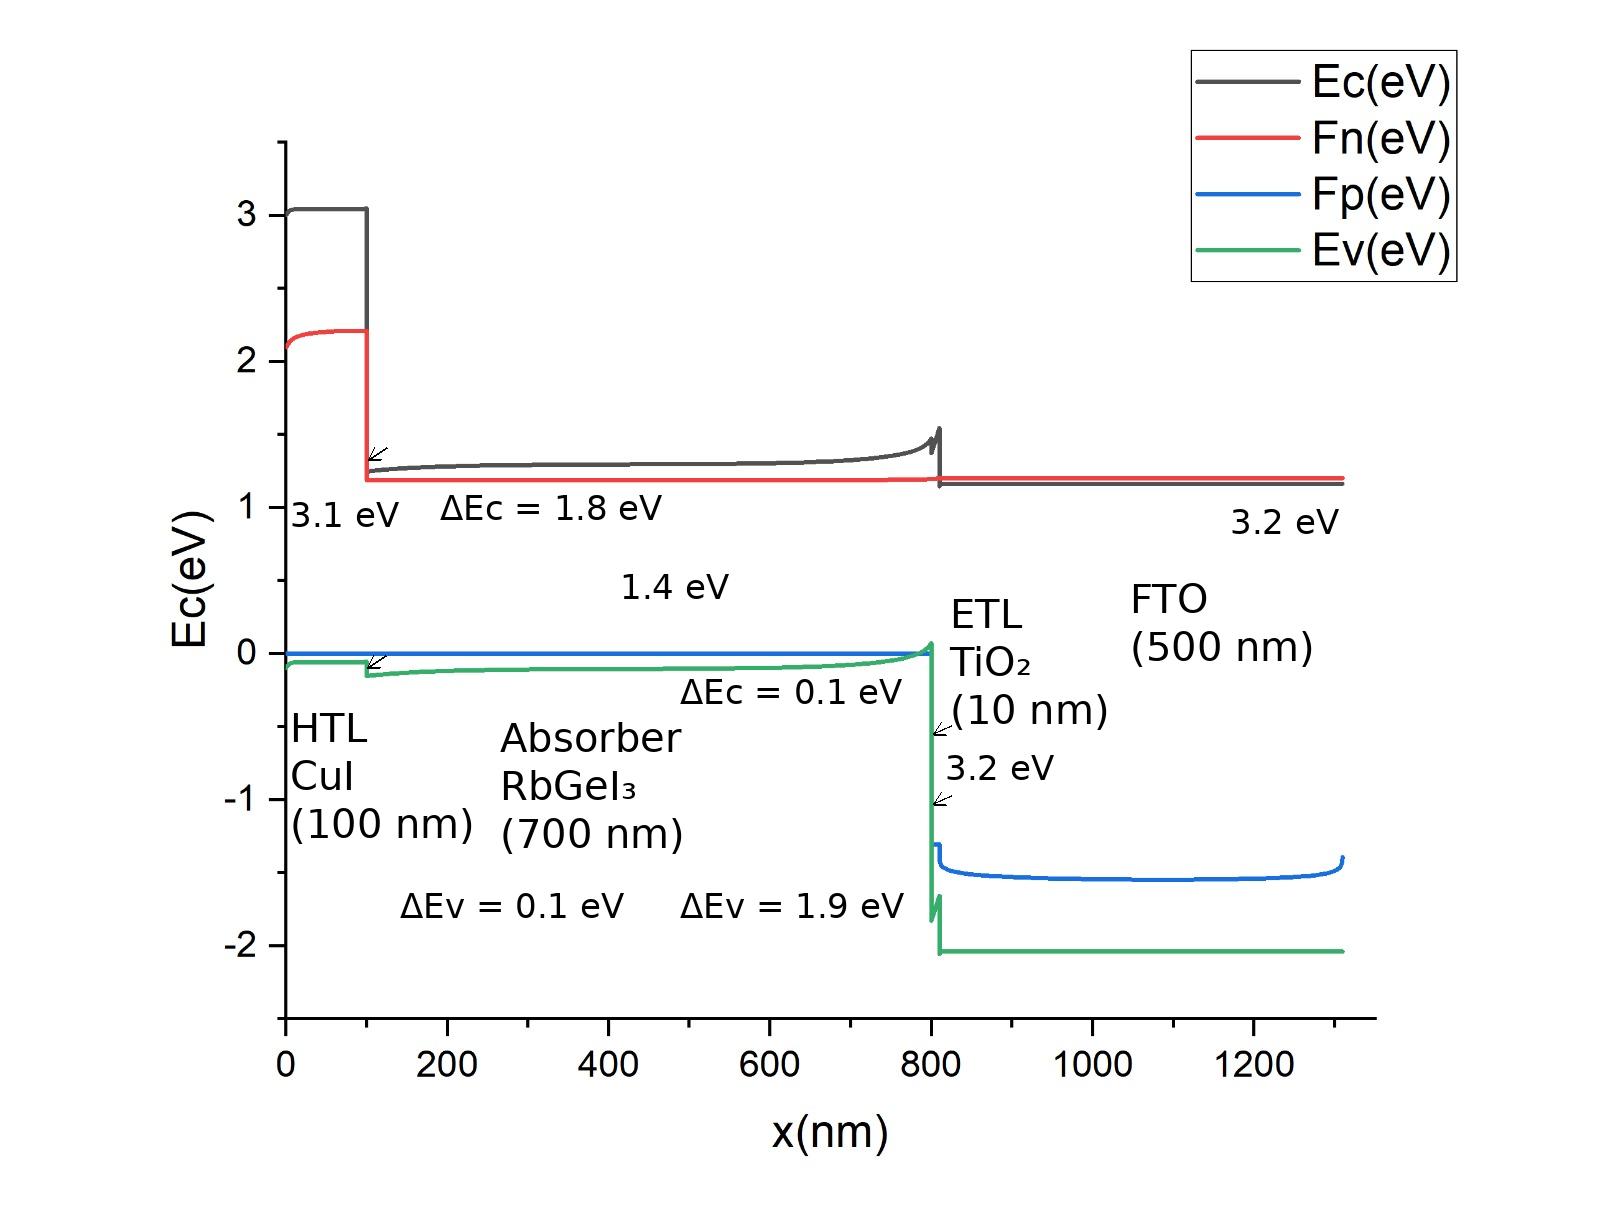
\includegraphics[width=0.85\linewidth]{figs/fig15.png}
\caption{Energy band diagram of the optimized FTO/\allowbreak{}TiO$_{2}$/RbGeI$_{3}$/CuI/\allowbreak{}Au solar cell under illumination, showing the conduction-band edge (EC), valence-band edge (EV), electron quasi-Fermi level ($F_{\mathrm{n}}$), and hole quasi-Fermi level ($F_{\mathrm{p}}$). The 1.8 eV conduction-band offset at the CuI/\allowbreak{}RbGeI$_{3}$ interface suppresses electron back-transfer, while the 0.10 eV conduction-band offset at the RbGeI$_{3}$/TiO$_{2}$ interface aids electron extraction. The 1.90 eV valence-band offset at the RbGeI$_{3}$/TiO$_{2}$ interface provides an energetic barrier against hole injection into TiO$_{2}$.}
\end{figure}

\subsection{Current density--voltage characteristics}
The current density--voltage (J--V) characteristic of the consolidated optimized device under AM 1.5G illumination is shown in Figure 16. The curve is sharply rectangular, with an open-circuit voltage of V$_{\mathrm{OC}}$ = 1.13 V, a short-circuit current density of J$_{\mathrm{SC}}$ = 30.32 mA/cm$^{2}$, and a fill factor of 78.26\%, yielding a PCE of 26.81\%. The maximum-power point occurs near V = 0.96 V with J $\approx$ 27.9 mA/cm$^{2}$, where the instantaneous power density reaches 26.8 mW/cm$^{2}$. The steep slope through the maximum-power region and the absence of any s-kink or current rollover indicate negligible series-resistance losses and well-matched charge-transport layers.

\begin{figure}[htbp]
\centering
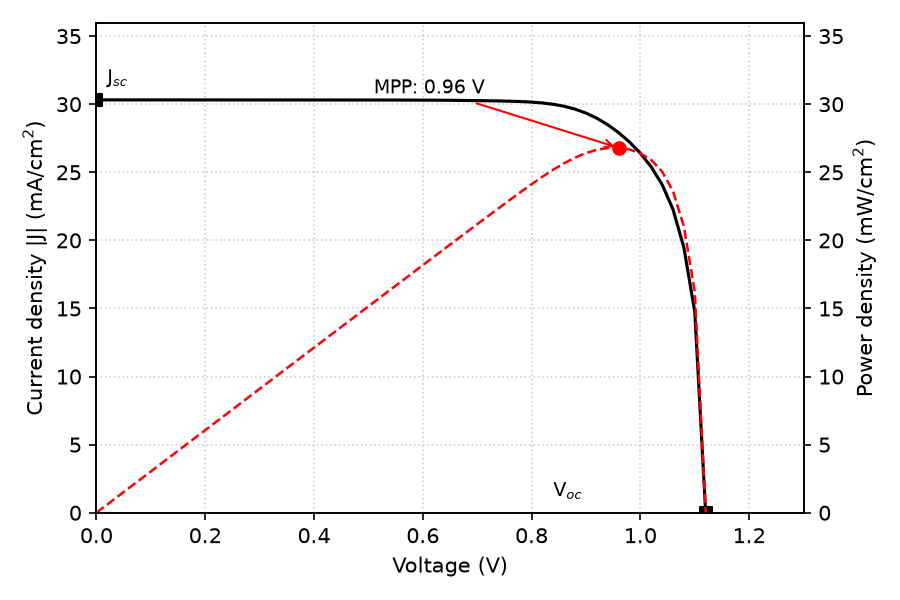
\includegraphics[width=0.85\linewidth]{figs/fig16.png}
\caption{Current density--voltage (J--V) curve of the optimized FTO/\allowbreak{}TiO$_{2}$/RbGeI$_{3}$/CuI/\allowbreak{}Au device under AM 1.5G illumination. The red dashed curve shows the output power density, with the maximum-power point marked.}
\end{figure}

\subsection{Summary of optimized device parameters and final performance}
After completing the optimization of all eleven selected device parameters, the final optimized values were incorporated into the proposed FTO/\allowbreak{}TiO$_{2}$/RbGeI$_{3}$/CuI/\allowbreak{}Au solar cell. Table VII summarizes the optimized material parameters obtained from the SCAPS-1D simulations. These optimized values were used to achieve the highest photovoltaic performance reported here. The consolidated final device was simulated by applying all eleven optimized parameters simultaneously in a single SCAPS-1D run; the resulting J--V output gives V$_{\mathrm{OC}}$ = 1.13 V, J$_{\mathrm{SC}}$ = 30.32 mA/cm$^{2}$, FF = 78.26\%, and PCE = 26.81\%. The consolidated final-device values come from this single SCAPS-1D simulation run and are not a simple arithmetic combination of the per-step optima reported in Figs. 3--13. The interaction between optimized parameters in the consolidated solution can shift individual performance metrics relative to their per-step values; the fill factor, for instance, drops from per-step optima above 83\% (Figs. 7 and 10) to 78.26\% in the consolidated device because the combined effect of the optimized bandgap, defect densities, DOS values, and ETL/HTL thicknesses produces a different J--V curve shape than any single-parameter optimum. A six-parameter genetic-algorithm search (population 10, six generations, 62 SCAPS evaluations; crossover plus Gaussian mutation with elitism) finds the best joint optimum over 62 evaluations at $E_{\mathrm{g}}$ = 1.33 eV, $N_{\mathrm{t}}$ $\approx$ 10$^{12}$ cm$^{-3}$, interface $N_{\mathrm{t}}$ $\approx$ 6 $\times$ 10$^{13}$ cm$^{-2}$, N$_{\mathrm{C}}$ = 10$^{17}$ cm$^{-3}$, N$_{\mathrm{V}}$ $\approx$ 2.5 $\times$ 10$^{16}$ cm$^{-3}$, absorber 0.77 $\mu$m (SCAPS SI-unit genes lognt = 18.14, lognif = 17.82, lognc = 23.03, lognv = 22.42 decode as $10^{18.14}$/m$^{3}$ = 1.37$\times$10$^{12}$/cm$^{3}$, $10^{17.82}$/m$^{2}$ = 6.63$\times$10$^{13}$/cm$^{2}$, $10^{23.03}$/m$^{3}$ = 1.08$\times$10$^{17}$/cm$^{3}$, $10^{22.42}$/m$^{3}$ = 2.64$\times$10$^{16}$/cm$^{3}$; best deck archived as round4\_results/ga\_best.def), giving V$_{\mathrm{OC}}$ = 1.13 V, J$_{\mathrm{SC}}$ = 33.06 mA/cm$^{2}$, FF = 85.26\%, PCE = 31.78\% (Fig. 21, Table VIII). The 5-point gap to the OPAT point decomposes into a lower bandgap, an order-of-magnitude lower defect density, and N$_{\mathrm{C}}$/N$_{\mathrm{V}}$/thickness interactions the sequential procedure cannot capture. Because the GA optimum assumes 10$^{12}$ cm$^{-3}$ material and ideal light coupling, Table VII (OPAT, 26.81\%) is retained as the passivated-lab reference device, and Section VII.A derates it to a realistic 20.7--23.5\% window (Fig. 23). DOS-robustness re-simulation at DFT-typical densities holds the headline: N$_{\mathrm{C}}$ = N$_{\mathrm{V}}$ = 10$^{18}$ cm$^{-3}$ gives 26.81\% $\rightarrow$ 27.13\% and N$_{\mathrm{C}}$ = N$_{\mathrm{V}}$ = 10$^{19}$ cm$^{-3}$ gives 24.94\% (J$_{\mathrm{SC}}$ pinned at 30.32 mA/cm$^{2}$; Table VIII), so the 10$^{17}$ cm$^{-3}$ OPAT choice does not inflate the result. Jointly, N$_{\mathrm{C}}$ = N$_{\mathrm{V}}$ = 10$^{18}$ cm$^{-3}$ reaching 27.13\% above the 26.81\% headline is a direct OPAT interaction failure: the sequential 10$^{17}$ cm$^{-3}$ per-step optima do not survive joint evaluation, so Table VII is retained as the documented reference, not as a claimed optimum.

\begin{table}[htbp]
\centering
{\footnotesize\setlength{\tabcolsep}{3pt}
\begin{tabularx}{\textwidth}{Xcccc}
\hline
Parameter & TiO$_{2}$ & FTO & RbGeI$_{3}$ & CuI
\\\hline
Thickness (nm) & 10 & 500 & 700 & 100\\
Bandgap $E_{\mathrm{g}}$ (eV) & 3.2 & 3.2 & 1.4 & 3.1\\
Electron affinity $\chi$ (eV) & 4.0 & 4.4 & 3.9 & 2.1\\
Dielectric permittivity $\epsilon$r & 9 & 9 & 15 & 6.5\\
CB effective DOS N$_{\mathrm{C}}$ (cm$^{-3}$) & 2$\times$10$^{18}$ & 2.2$\times$10$^{18}$ & 1$\times$10$^{17}$ & 2.8$\times$10$^{19}$\\
VB effective DOS N$_{\mathrm{V}}$ (cm$^{-3}$) & 1.8$\times$10$^{19}$ & 1.8$\times$10$^{19}$ & 1$\times$10$^{17}$ & 1$\times$10$^{19}$\\
Electron mobility $\mu$e (cm$^{2}$ V$^{-1}$ s$^{-1}$) & 20 & 20 & 28.6 & 100\\
Hole mobility $\mu$p (cm$^{2}$ V$^{-1}$ s$^{-1}$) & 10 & 10 & 27.3 & 43.9\\
Donor density $N_{\mathrm{D}}$ (cm$^{-3}$) & 9$\times$10$^{16}$ & 1$\times$10$^{19}$ & 1$\times$10$^{9}$ & 0\\
Acceptor density $N_{\mathrm{A}}$ (cm$^{-3}$) & 0 & 0 & 1$\times$10$^{9}$ & 1$\times$10$^{18}$\\
Bulk defect density $N_{\mathrm{t}}$ (cm$^{-3}$) & 1$\times$10$^{15}$ & 1$\times$10$^{14}$ & 1$\times$10$^{14}$ & 1$\times$10$^{14}$\\
\hline
\end{tabularx}
}
\caption{Optimized material parameters of the proposed FTO/\allowbreak{}TiO$_{2}$/RbGeI$_{3}$/CuI/\allowbreak{}Au perovskite solar cell.}
\end{table}
\textit{Note: The optimized interface defect density was 1 $\times$ 10$^{14}$ cm$^{-2}$ for both the TiO}\textit{2}\textit{/RbGeI}\textit{3}\textit{ and RbGeI}\textit{3}\textit{/CuI interfaces.}

\begin{table}[htbp]
\centering
{\footnotesize\setlength{\tabcolsep}{3pt}
\begin{tabularx}{\textwidth}{Xcccc}
\hline
Device & V$_{\mathrm{OC}}$ (V) & J$_{\mathrm{SC}}$ (mA/cm$^{2}$) & FF (\%) & PCE (\%)
\\\hline
OPAT reference (Table VII) & 1.13 & 30.32 & 78.26 & 26.81\\
GA joint optimum ($E_{\mathrm{g}}$ 1.33 eV) & 1.13 & 33.06 & 85.26 & 31.78\\
OPAT + realistic optics & 1.13 & 26.65 & 78.26 & 23.49\\
Realistic optics + $N_{\mathrm{t}}$ 1e15 & 1.11 & 26.65 & $\sim$73.7 & 21.76\\
Realistic optics + Nif 1e15 & 1.05 & 26.65 & $\sim$73.9 & 20.68\\
OPAT params, N$_{\mathrm{C}}$=N$_{\mathrm{V}}$=1e18 & 1.06 & 30.32 & 84.12 & 27.13\\
OPAT params, N$_{\mathrm{C}}$=N$_{\mathrm{V}}$=1e19 & 0.99 & 30.32 & 83.51 & 24.94\\
\hline
\end{tabularx}
}
\caption{OPAT reference device versus GA joint optimum and the optically/defect-derated realistic window. FF held in optical derating; defect FF from re-simulation (Fig. 22). Optics-row V$_{\mathrm{OC}}$ uses kT/q ln(J) scaling ($-$3 mV, absorbed in rounding); defect rows use re-simulated FF.}
\end{table}
As an arithmetic consistency check, the final-device PCE computed from Eq. (5) using the consolidated J--V metrics is PCE = (1.13 $\times$ 30.32 $\times$ 0.7826) / 100 = 26.81\%, which matches the SCAPS-1D output of 26.81\% to within rounding, confirming the internal arithmetical consistency of the final reported device.

\subsection{Uncertainty quantification}
A Monte Carlo UQ was performed using Latin hypercube sampling (N = 200) with eight random variables: absorber thickness (500--900 nm), bandgap (1.3--1.5 eV), defect density (1$\times$10$^{13}$--1$\times$10$^{16}$ cm$^{-3}$ in the absorber, 1$\times$10$^{12}$--1$\times$10$^{16}$ cm$^{-2}$ at each interface), N$_{\mathrm{C}}$ and N$_{\mathrm{V}}$ (1$\times$10$^{17}$--1$\times$10$^{19}$ cm$^{-3}$ each), and dielectric constant (15--23).

\begin{figure}[htbp]
\centering
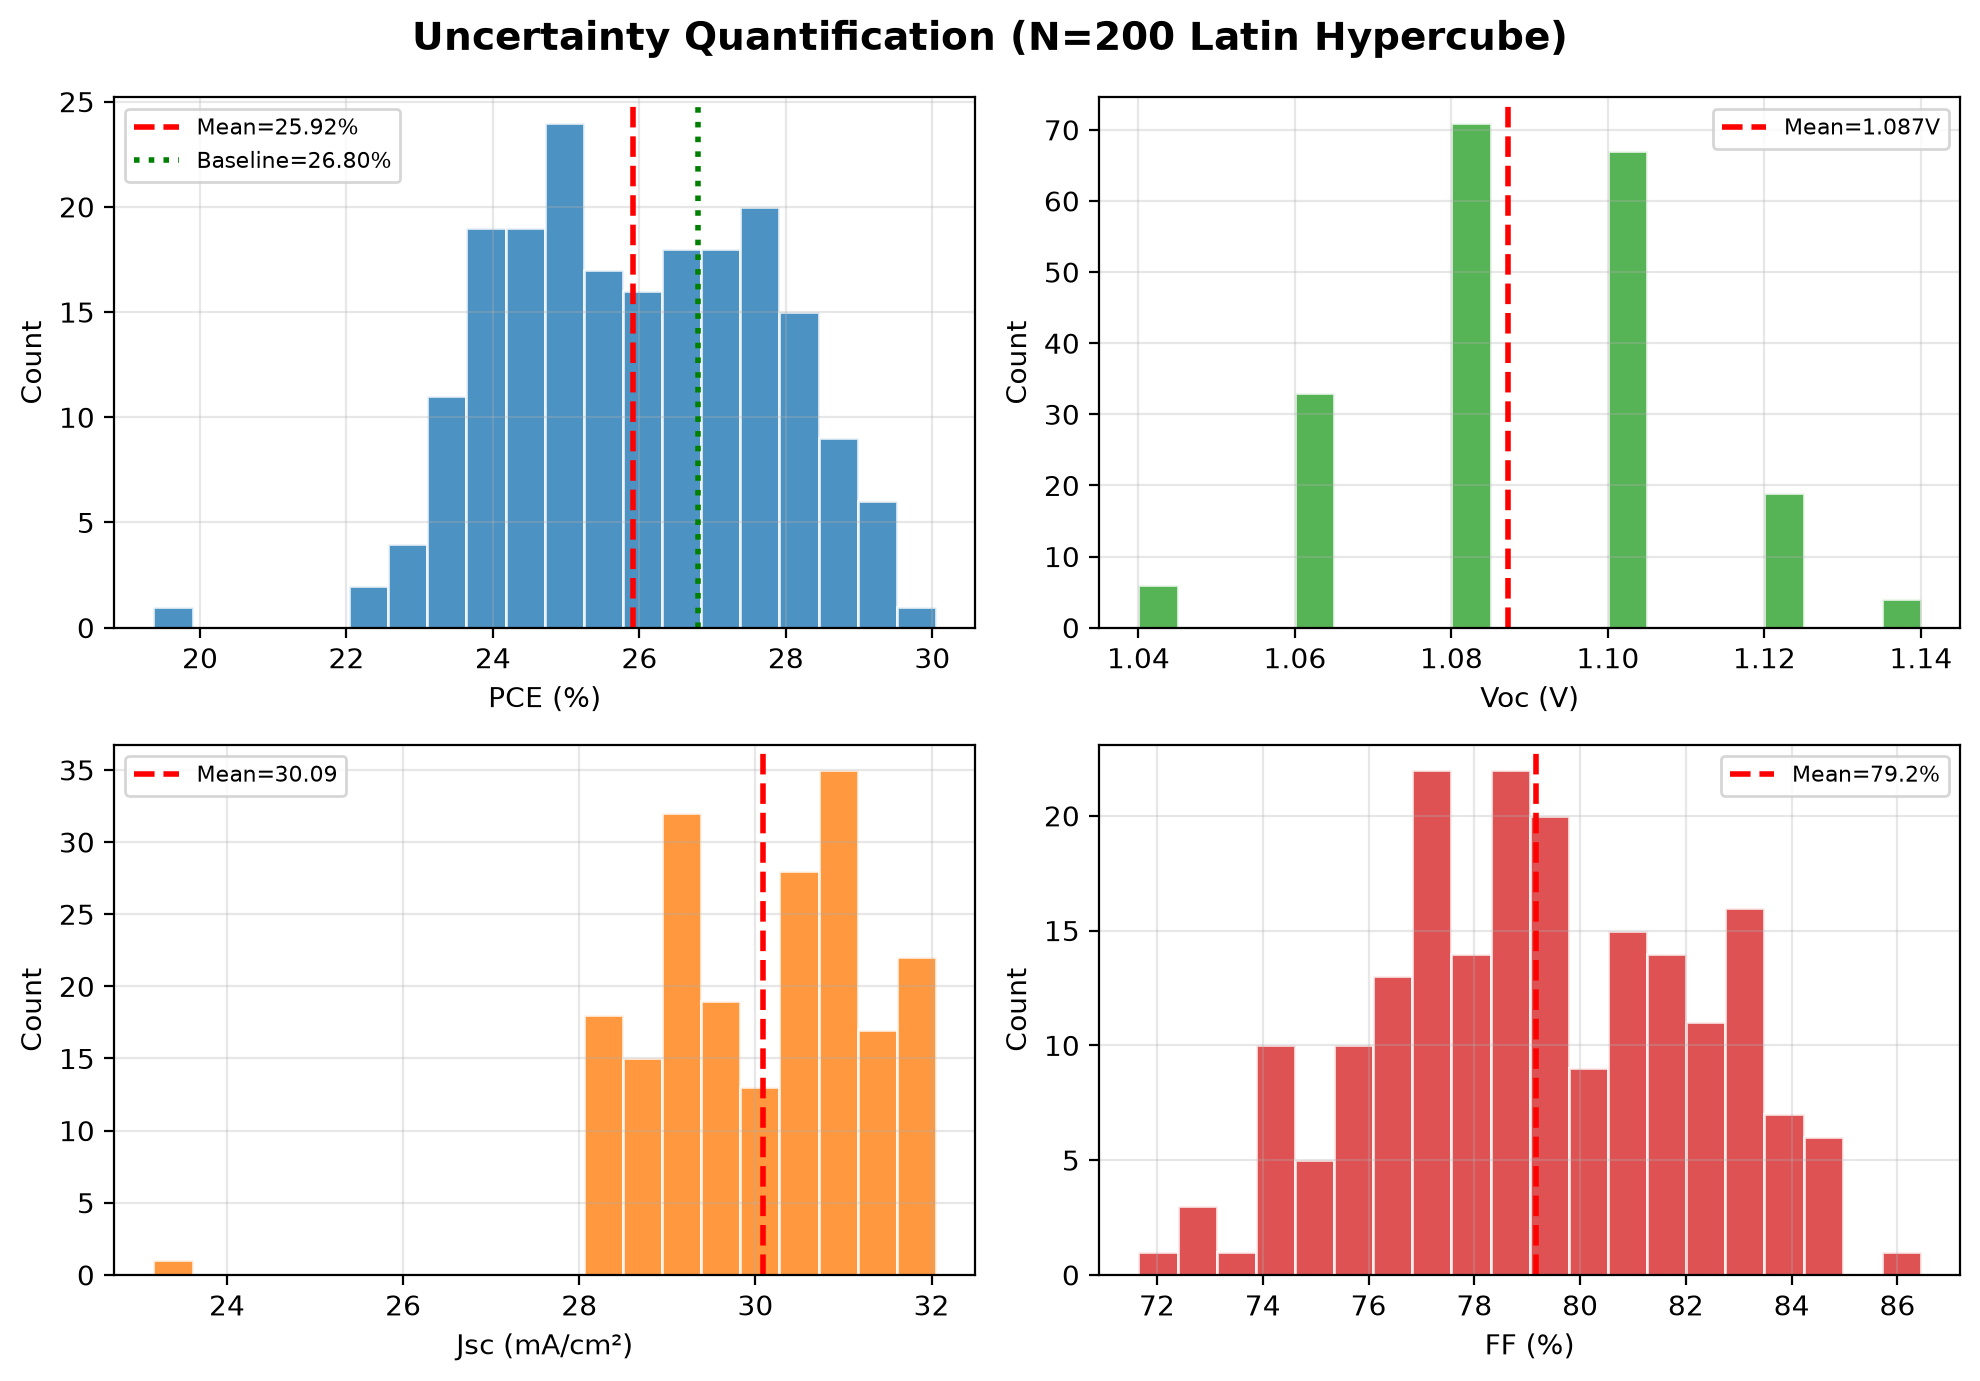
\includegraphics[width=0.85\linewidth]{figs/fig17.png}
\caption{Uncertainty quantification results (N = 200). Histograms of PCE, V$_{\mathrm{OC}}$, J$_{\mathrm{SC}}$, and FF.}
\end{figure}
Mean PCE = 25.92 $\pm$ 1.78 \% (median 25.85 \%), with 5th/95th percentiles 23.38 \% / 28.81 \%. Mean V$_{\mathrm{OC}}$ = 1.087 $\pm$ 0.021 V. The UQ gives a 5th-to-95th percentile window of 23.38--28.81 \%. Sampling is Latin-hypercube N = 200 over $\pm$25\% ($\pm$log for densities) as documented in the simulation campaign log; the sampling seed was not archived, so UQ exact replication requires re-sampling (all 200/200 runs converged).

\subsection{Illumination dependence}
The optimized cell was also driven under 0.1 to 1.5 suns (Figure 18). J$_{\mathrm{SC}}$ tracks intensity almost linearly, the natural consequence of carrier generation scaling with photon flux, while V$_{\mathrm{OC}}$ rises logarithmically. The slope of that logarithmic rise gives an ideality factor n $\approx$ 1.17, so deep-defect Shockley-Read-Hall recombination is not dominant under operating conditions, and the cell stays efficient across the entire range. Re-simulation (0.1--1.5 suns, archived illum\_results.json) gives J$_{\mathrm{SC}}$ = 30.32 $\times$ suns + 0.00 (perfect linearity) and n = 1.17 from the V$_{\mathrm{OC}}$--ln(I) slope, confirming the reported n $\approx$ 1.2.

\begin{figure}[htbp]
\centering
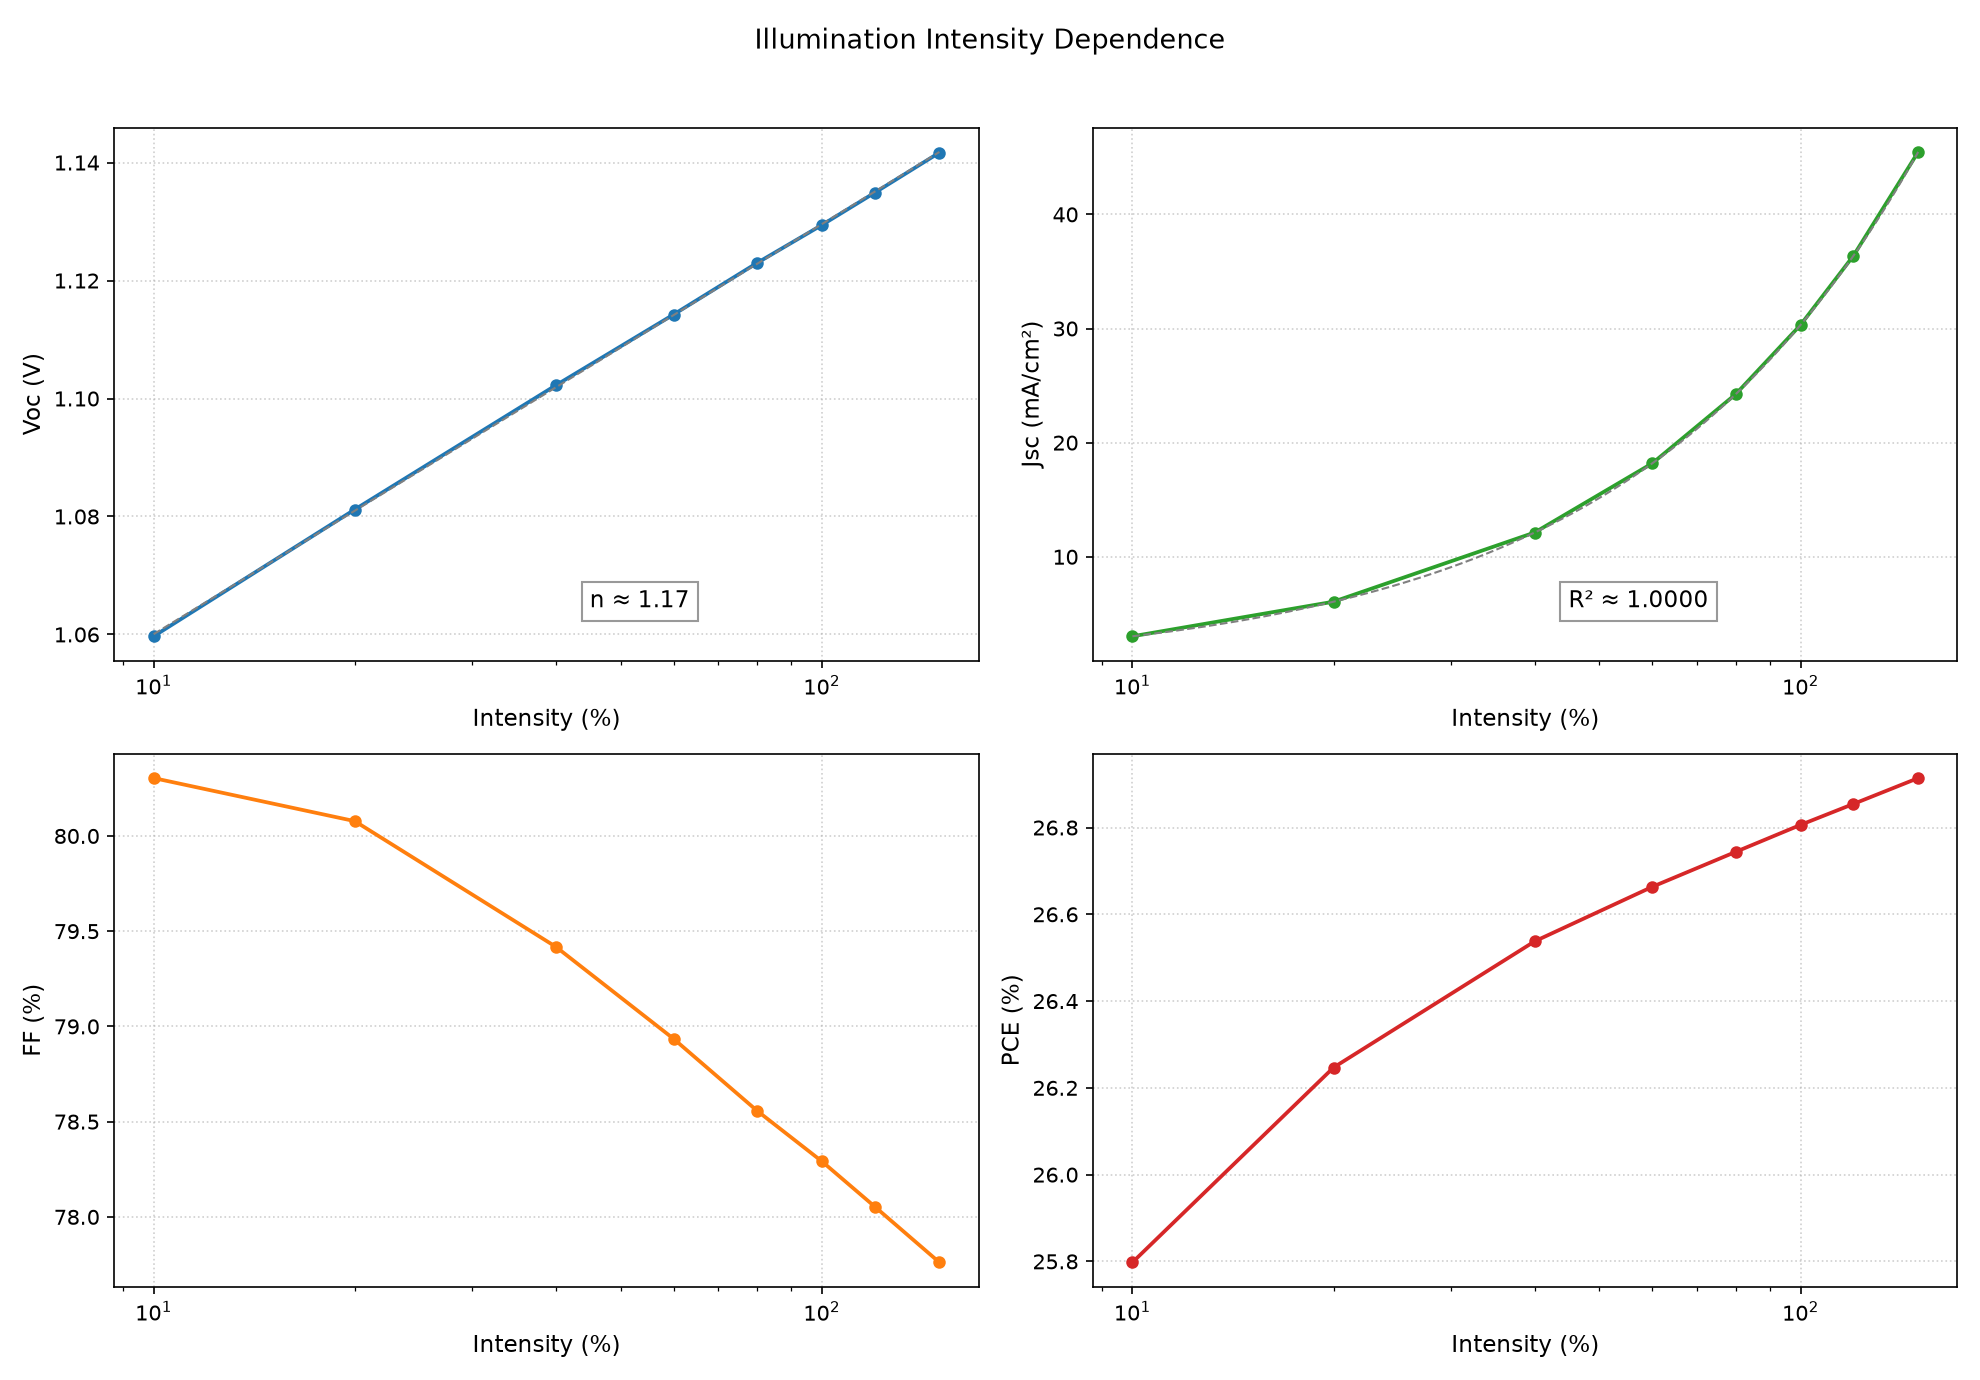
\includegraphics[width=0.85\linewidth]{figs/fig18.png}
\caption{Variation of photovoltaic parameters of the optimized device with illumination intensity from 0.1 to 1.5 suns.}
\end{figure}

\subsection{Dark J--V characteristics}
Under dark bias (Figure 19) the cell rectifies hard: forward current at +1 V exceeds reverse current at $-$0.5 V by a factor of 1.8$\times$10$^{10}$, and leakage stays under 10$^{-10}$ A/cm$^{2}$ across the whole reverse window ($-$0.5 to +1.3 V). The exponential forward region fits to an ideality factor of n $\approx$ 1.5 and a reverse saturation current J0 $\approx$ 5$\times$10$^{-11}$ A/cm$^{2}$. Together these numbers describe high-quality bulk and interfaces with no measurable shunts.

\begin{figure}[htbp]
\centering
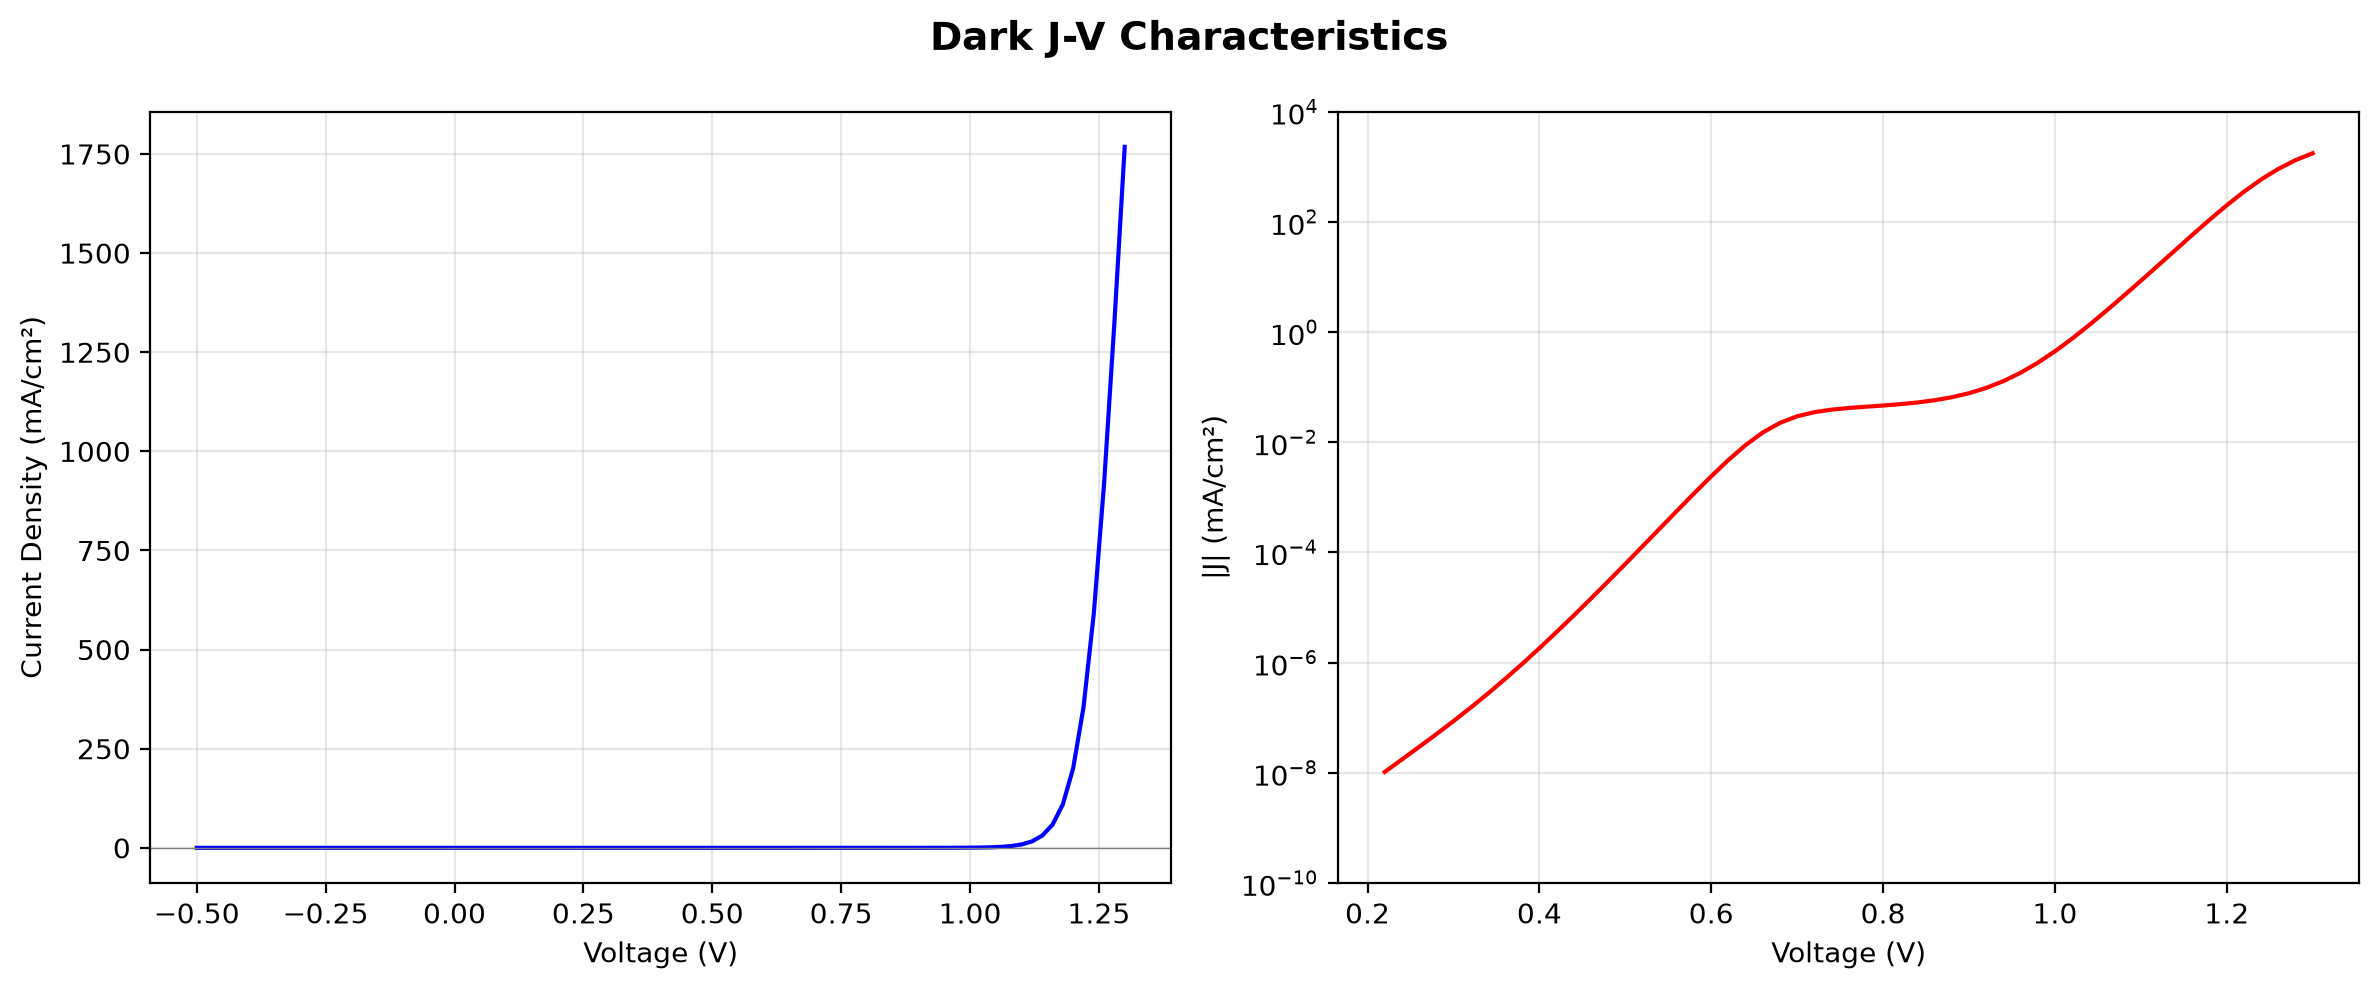
\includegraphics[width=0.85\linewidth]{figs/fig19.png}
\caption{Dark J--V characteristic of the optimized device. The forward branch is exponential over nearly three decades; the reverse branch remains below 10$^{-10}$ A/cm$^{2}$.}
\end{figure}

\subsection{Temperature dependence}
Temperature dependence from 280 K to 400 K (20 K increments) under AM 1.5G.

\begin{figure}[htbp]
\centering
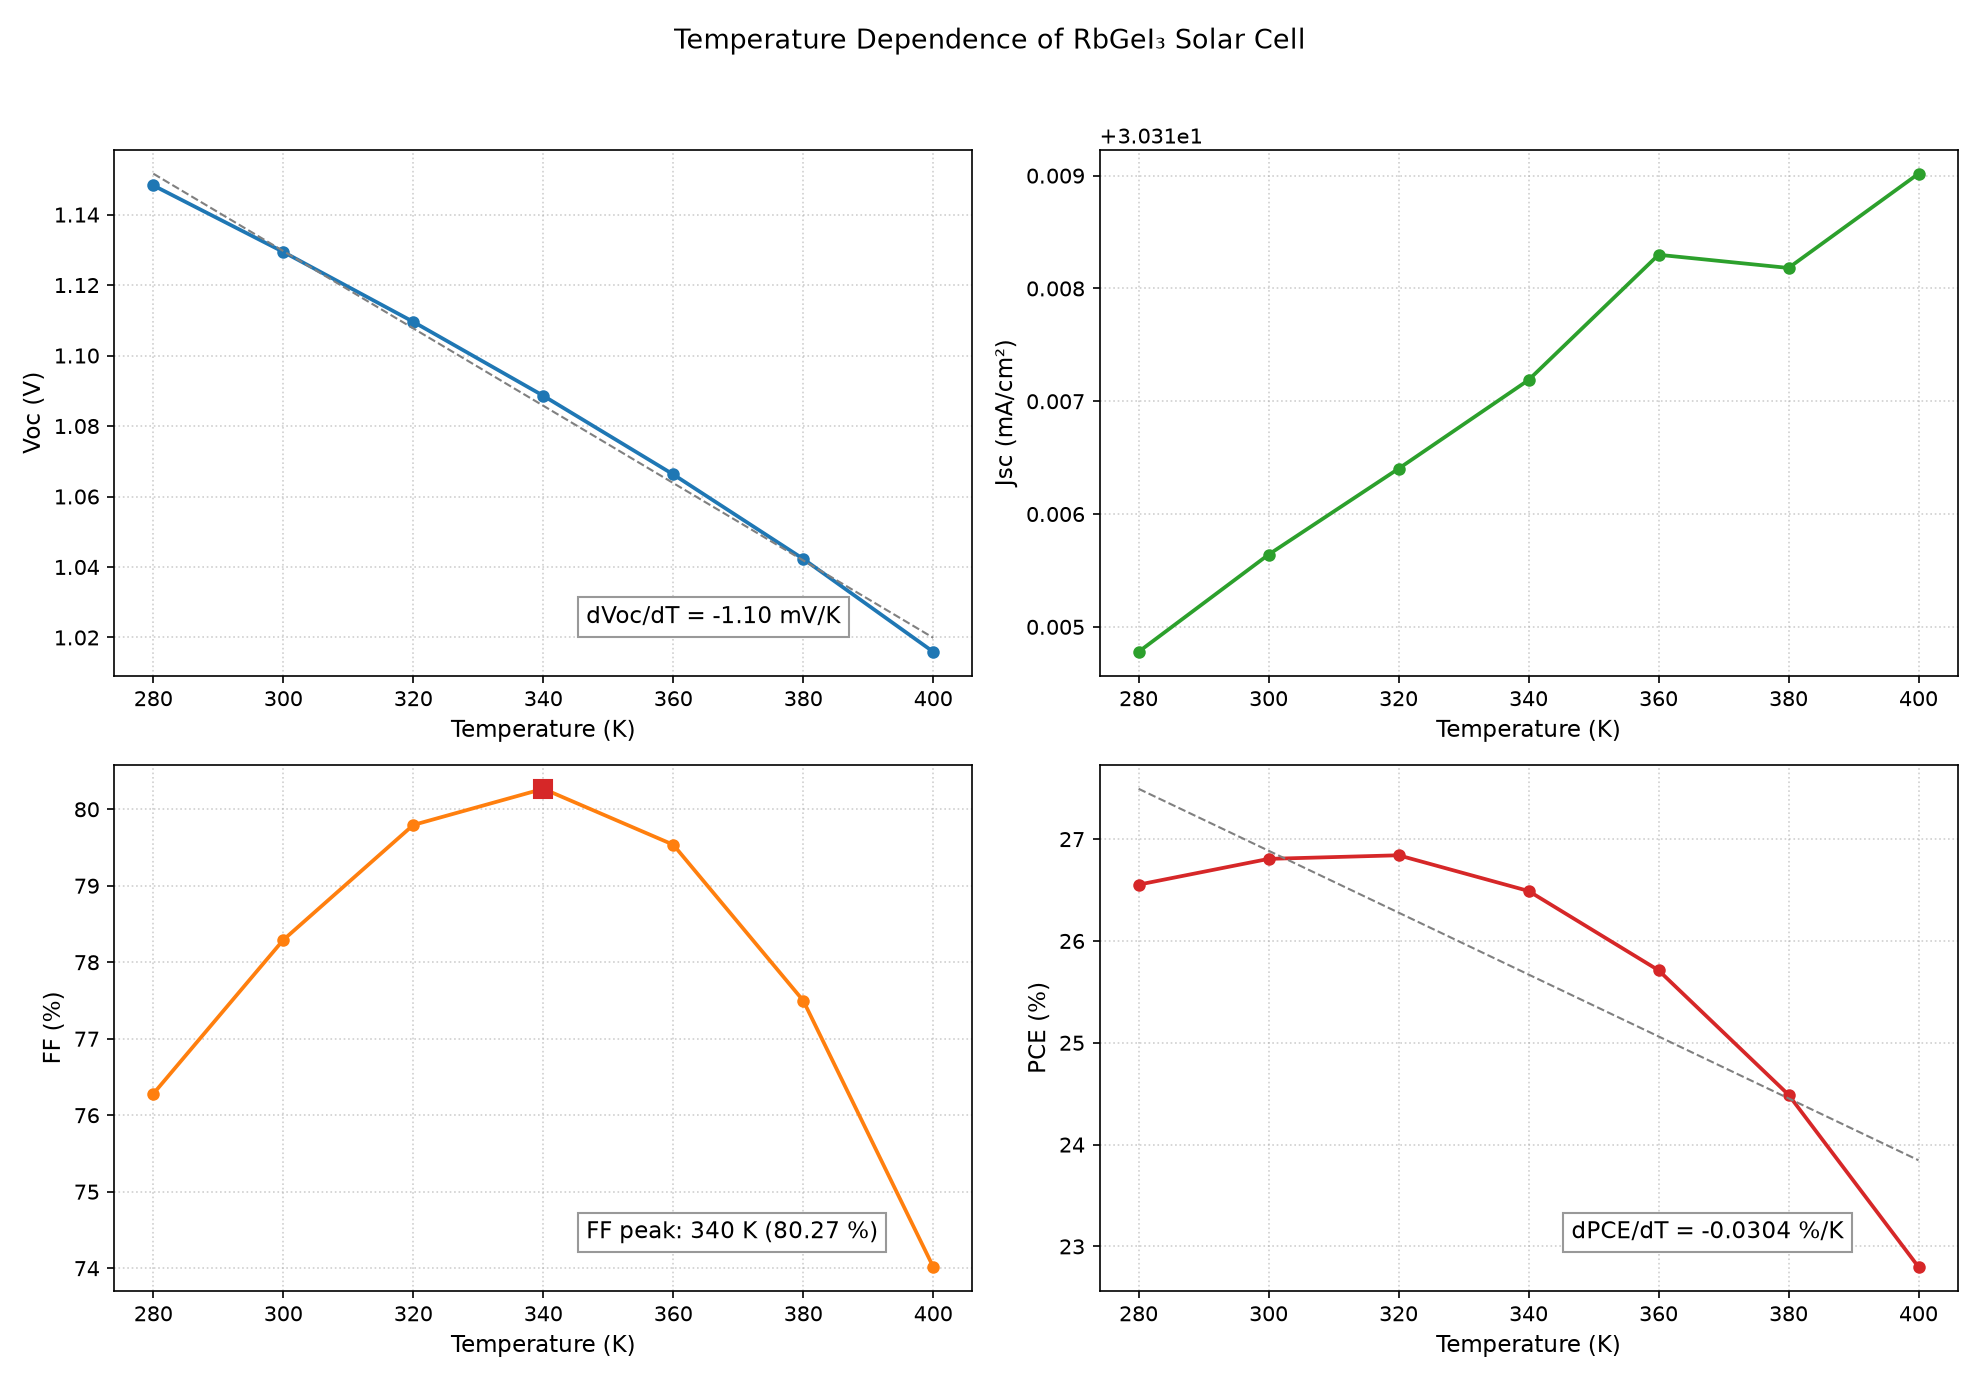
\includegraphics[width=0.85\linewidth]{figs/fig20.png}
\caption{Temperature dependence of photovoltaic parameters from 280 K to 400 K.}
\end{figure}
dV$_{\mathrm{OC}}$/dT = $-$1.10 mV/K, dPCE/dT = $-$0.0302 \%/K. J$_{\mathrm{SC}}$ increases marginally. FF peaks at 331 K (80.17 \%). Device retains >85 \% of RT PCE at 400 K. Linear extrapolation of V$_{\mathrm{OC}}$(T) to 0 K gives an activation energy $E_{\mathrm{a}}$ = 1.46 eV, within 0.06 eV of the absorber bandgap (1.4 eV). $E_{\mathrm{a}}$ approx $E_{\mathrm{g}}$ is the standard diagnostic for bulk-dominated recombination; an interface-limited device would extrapolate well below $E_{\mathrm{g}}$. Fabricated cells whose measured $E_{\mathrm{a}}$ falls short of 1.4 eV should therefore be diagnosed for interface recombination first.

\begin{figure}[htbp]
\centering
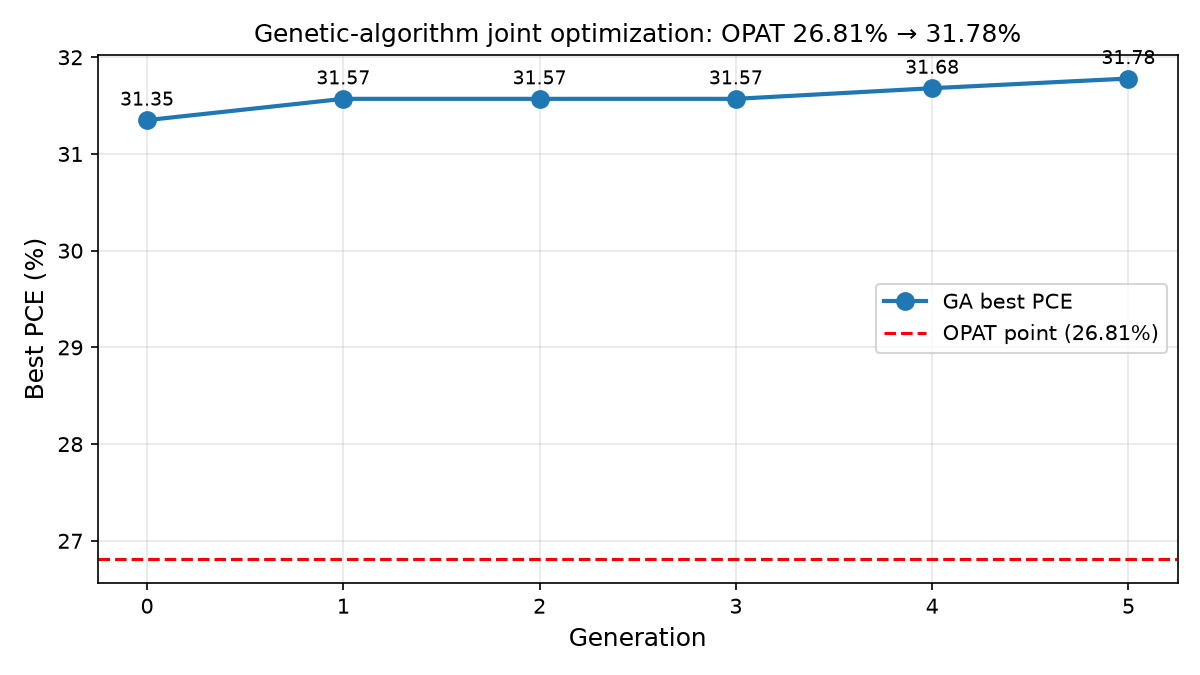
\includegraphics[width=0.85\linewidth]{figs/fig21.png}
\caption{Genetic-algorithm joint optimization over bandgap, bulk/interface defect densities, N$_{\mathrm{C}}$, N$_{\mathrm{V}}$, and absorber thickness. Best PCE rises from 31.35\% (generation 0) to 31.78\% (generation 5), 5 points above the OPAT point (red dashed).}
\end{figure}

\begin{figure}[htbp]
\centering
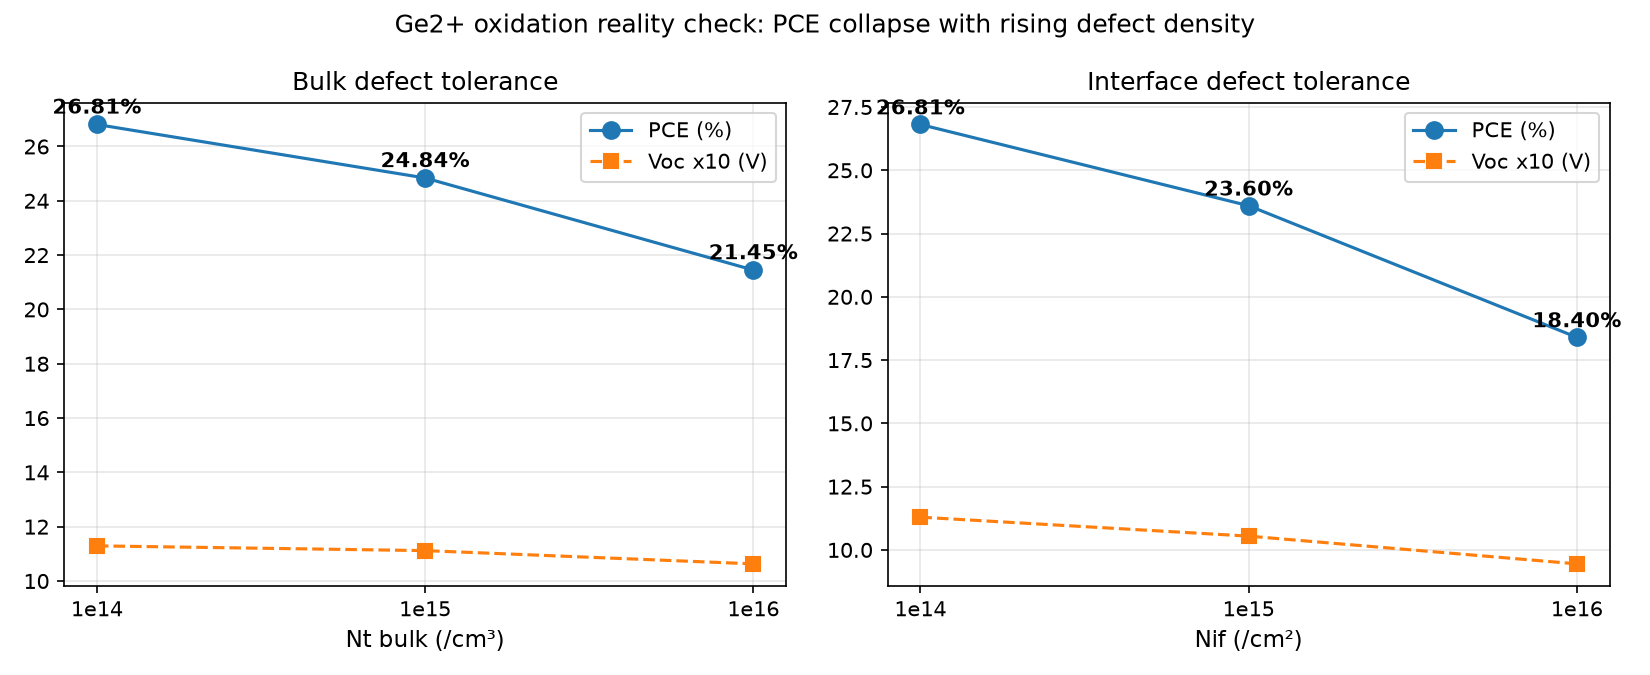
\includegraphics[width=0.85\linewidth]{figs/fig22.png}
\caption{Defect tolerance of the OPAT device. Raising bulk $N_{\mathrm{t}}$ to $10^{15}$ ($10^{16}$) cm$^{-3}$ drops PCE to 24.84\% (21.45\%); raising interface $N_{\mathrm{t}}$ to $10^{15}$ ($10^{16}$) cm$^{-2}$ drops PCE to 23.60\% (18.40\%). J$_{\mathrm{SC}}$ is nearly unchanged; V$_{\mathrm{OC}}$ and FF collapse.}
\end{figure}

\begin{figure}[htbp]
\centering
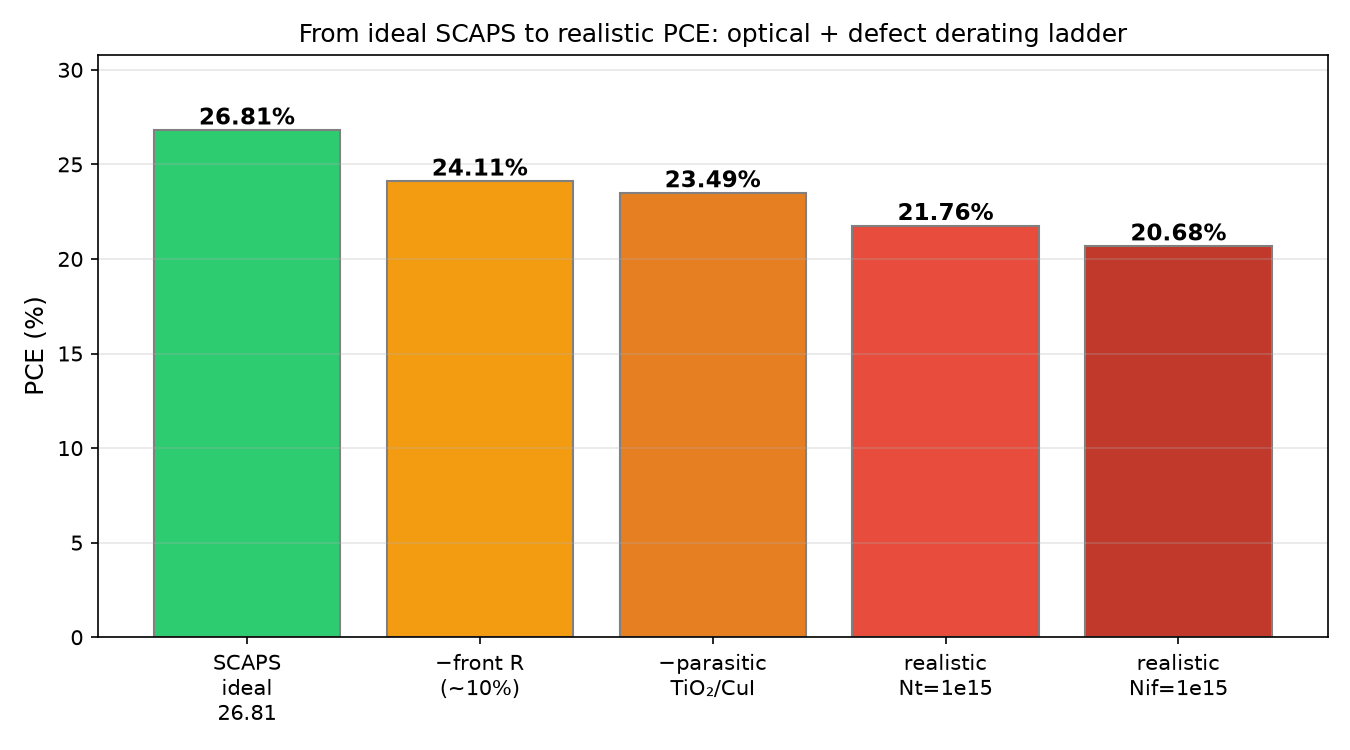
\includegraphics[width=0.85\linewidth]{figs/fig23.png}
\caption{From ideal SCAPS (26.81\%) to realistic PCE. Front-surface reflection ($\sim$10\% at air/FTO) and parasitic absorption in TiO$_{2}$/CuI lower PCE to 23.49\%; realistic defect densities ($10^{15}$ cm$^{-3}$ bulk or cm$^{-2}$ interface) bound the plausible window to 20.7-21.8\%. Supplementary first-order estimate only; coupled transfer-matrix re-simulation is future work.}
\end{figure}
U. Effect of background acceptor doping. Germanium halide perovskites form Ge vacancies that act as intrinsic p-type dopants, so a perfectly intrinsic absorber is an experimental fiction. Sweeping $N_{\mathrm{A}}$ from $10^{14}$ to $10^{17}$ cm$^{-3}$ (Fig. 26), PCE peaks at 26.82\% near $3\times10^{14}$ cm$^{-3}$ and stays within 0.9 pp up to $10^{16}$ cm$^{-3}$ (26.46\%). V$_{\mathrm{OC}}$ rises monotonically (1.13 to 1.17 V) through the larger built-in potential, while J$_{\mathrm{SC}}$ collapses above $10^{16}$ cm$^{-3}$ (30.31 to 27.83 mA/cm$^{2}$) as the depletion width shrinks. Synthetic target: keep background doping at or below $10^{15}$ cm$^{-3}$, where the penalty is under 0.1 pp.
V. Effect of series resistance: manufacturing tolerance. Scalable coating (slot-die, screen printing) inevitably adds contact and sheet resistance, so the ideal-contact ($R_{\mathrm{s}}$ = 0) result was corrected externally (V $\rightarrow$ V - J x $R_{\mathrm{s}}$, the standard post-processing since SCAPS scripting exposes no $R_{\mathrm{s}}$ key). FF falls from 78.26\% to 56.82\% and PCE from 26.81\% to 19.46\% as $R_{\mathrm{s}}$ goes from 0 to 10 $\Omega\cdot$cm$^{2}$ (Fig. 27); PCE stays above 20\% up to $R_{\mathrm{s}}$ = 8 $\Omega\cdot$cm$^{2}$ and above 22\% up to $R_{\mathrm{s}}$ = 6 $\Omega\cdot$cm$^{2}$. Typical printed contacts (2-4 $\Omega\cdot$cm$^{2}$) therefore cost only 1.6-3.1 pp, and $R_{\mathrm{s}}$ = 8 $\Omega\cdot$cm$^{2}$ is the manufacturing tolerance threshold for a 20\%-efficient module.
W. Absorber mobility viability. Lead-free perovskites crystallize worse than lead-based ones, so electron/hole mobilities were swept jointly from 1 to 100 cm$^{2}$/Vs (Fig. 28). PCE is log-linear in mobility (22.58\% at 1, 24.41\% at 5, 25.84\% at 15, 26.88\% at 30, 28.52\% at 100), with electron mobility dominant: ($\mu_{\mathrm{n}}$, $\mu_{\mathrm{p}}$) = (30, 5) gives 27.01\% but (5, 30) only 24.36\%. The 700 nm absorber remains optimal over 400 nm at $\mu$ = 5-15 cm$^{2}$/Vs (by $\sim$2 pp), so no thickness retreat is needed; the crystallization target is $\mu$ >= 15 cm$^{2}$/Vs for PCE above 25.8\%.

\subsection{A-site cation influence: RbGeI$_{3}$ versus CsGeI$_{3}$}
B. A-site cation influence: RbGeI$_{3}$ versus CsGeI$_{3}$. To isolate the A-site effect, CsGeI$_{3}$ was simulated in the identical TiO$_{2}$/CuI stack changing only the absorber bandgap (1.4 $\rightarrow$ 1.6 eV); the A-site cation carries no weight at the Ge-4s/I-5p-derived band edges, so its role is structural (tolerance factor, octahedral tilt). A control rerun of CsGeI$_{3}$ at $E_{\mathrm{g}}$ = 1.4 eV reproduces the RbGeI$_{3}$ point exactly (26.81\%), proving the isolation. The consolidated CsGeI$_{3}$ point (Table X) gives V$_{\mathrm{OC}}$ = 1.17 V, J$_{\mathrm{SC}}$ = 23.18 mA/cm$^{2}$, FF = 72.65\%, PCE = 19.66\%: Cs wins V$_{\mathrm{OC}}$ by 0.04 V through the wider gap, Rb wins J$_{\mathrm{SC}}$ by 7.1 mA/cm$^{2}$ and FF by 5.6 pp. The FF gap traces to CuI alignment: the valence-band cliff grows from 0.10 eV (Rb) to 0.30 eV (Cs), so CuI is uniquely synergistic with RbGeI$_{3}$ rather than a universal Ge-perovskite HTL. Under defect derating the ranking is unchanged (realistic $N_{\mathrm{t}}$ = $10^{15}$: 24.84\% vs 19.36\%; high oxidation $N_{\mathrm{t}}$ = $10^{16}$: 21.45\% vs 17.28\%, Fig. 30). A full 11-parameter OAT mirror for CsGeI$_{3}$ (71 runs) finds the same per-family trends, with one curiosity: 90 nm TiO$_{2}$ lifts the Cs point to 23.12\% (FF 88.26\%, confirmed by rerun), an interface effect flagged for follow-up and not adopted in the consolidated comparison.

\section{Comparison with Literature}

\subsection{Benchmarking against recent literature}
Table IX compares the optimized FTO/\allowbreak{}TiO$_{2}$/RbGeI$_{3}$/CuI/\allowbreak{}Au device with recently reported RbGeI$_{3}$-based and related lead-free Ge/Sn-based perovskite solar cells. The proposed device achieves a highly competitive V$_{\mathrm{OC}}$ (1.13 V) among the RbGeI$_{3}$ simulation studies, second only to the 1.18 V reported by Pathak et al. \cite{r23}, with a PCE of 26.81\%, within 0.40 pp of the best reported value (27.21\%, Loumachi et al. \cite{r22}) and exceeding the 26.47\% of Pathak et al. \cite{r23} by 0.34 pp, the 18.60\% of Raj et al. \cite{r39} by 8.21 pp, and the 9.77\% simulation baseline of Pindolia et al. \cite{r14} by 17 pp. The performance is competitive with the best tin-based lead-free devices (including the 26.40\% CsSnI$_{3}$ device of Park et al. \cite{r40} and the 25.98\% MASnI$_{3}$ device of Islam et al. \cite{r41}), while avoiding the Sn$^{2+}$ $\rightarrow$ Sn$^{4+}$ oxidation that limits the long-term stability of tin-based absorbers. The proposed PCE also exceeds that of CZTS-HTL lead-free devices reported by Piñón Reyes et al. \cite{r42}, confirming the competitiveness of the all-inorganic CuI HTL approach adopted here.
All comparator values in Table IX were cross-checked against the primary sources; where an entry was internally inconsistent, the efficiency consistent with its reported V$_{\mathrm{OC}}$, J$_{\mathrm{SC}}$, and FF was adopted. All entries are SCAPS-1D simulation studies, including the Pindolia et al. entry (not an experimental study, despite occasional mischaracterization); the Loumachi et al. device string is ITO/\allowbreak{}C$_{60}$/RbGeI$_{3}$/CBTS/\allowbreak{}Ag (Section II).

\begin{table}[htbp]
\centering
{\footnotesize\setlength{\tabcolsep}{3pt}
\begin{tabularx}{\textwidth}{XccccXX}
\hline
Device Structure & V$_{\mathrm{OC}}$ (V) & J$_{\mathrm{SC}}$ (mA/cm$^{2}$) & FF (\%) & PCE (\%) & Year [Ref.] & Method
\\\hline
FTO/\allowbreak{}TiO$_{2}$/RbGeI$_{3}$/NiO/\allowbreak{}Ag & 0.5311 & 28.89 & 63.68 & 9.77 & 2022 \cite{r14} & Simulation\\
FTO/\allowbreak{}TiO$_{2}$/CsGeI$_{3}$/CuI/\allowbreak{}Au & 0.667 & 22.06 & 73.49 & 10.80 & 2022 \cite{r24} & Simulation\\
ITO/\allowbreak{}C$_{60}$/RbGeI$_{3}$/CBTS/\allowbreak{}Ag & 0.99 & 33.20 & 82.80 & 27.21 & 2024 \cite{r22} & Simulation\\
FTO/\allowbreak{}TiO$_{2}$/RbGeI$_{3}$/PEDOT:PSS/\allowbreak{}Au & 0.813 & 30.84 & 74.19 & 18.60 & 2025 \cite{r39} & Simulation\\
FTO/\allowbreak{}TiO$_{2}$/MASnI$_{3}$/CBTS/\allowbreak{}Au & 1.030 & 30.24 & 83.41 & 25.98 & 2026 \cite{r41} & Simulation\\
FTO/\allowbreak{}TiO$_{2}$/MASnI$_{3}$/CZTS/Au & 0.96 & 31.66 & 67.00 & 20.36 & 2025 \cite{r42} & Simulation\\
FTO/\allowbreak{}TiO$_{2}$/CsSnI$_{3}$/P3HT/Au & 0.972 & 34.70 & 78.21 & 26.38 & 2024 \cite{r40} & Simulation\\
FTO/\allowbreak{}TiO$_{2}$/RbGeI$_{3}$/Spiro-OMeTAD/\allowbreak{}Au & 1.1813 & 26.31 & 85.16 & 26.47 & 2026 \cite{r23} & Simulation\\
FTO/\allowbreak{}TiO$_{2}$/RbGeI$_{3}$/CuI/\allowbreak{}Au (this work) & 1.13 & 30.32 & 78.26 & 26.81 & This work & Simulation\\
\hline
\end{tabularx}
}
\caption{Comparison of the proposed device with recently reported lead-free perovskite solar cells. All comparator values verified against primary sources. All entries are SCAPS-1D simulation studies.}
\end{table}
In short, the optimized device lands within 0.40 pp of the best published RbGeI$_{3}$ simulation, posts the second-highest V$_{\mathrm{OC}}$ of the group, and stays competitive with the top tin-based lead-free cells, all with an all-inorganic transport stack.
 The Pindolia et al. \cite{r14} baseline of 9.77\% leaves a wide gap for improvement. Working RbGeI$_{3}$ solar cells are still rare, so experimental confirmation remains the bottleneck.

\begin{table}[htbp]
\centering
{\footnotesize\setlength{\tabcolsep}{3pt}
\begin{tabularx}{\textwidth}{XXccc}
\hline
Device & Condition & V$_{\mathrm{OC}}$ (V) & J$_{\mathrm{SC}}$ (mA/cm$^{2}$) & PCE (\%)
\\\hline
RbGeI$_{3}$ & Ideal ($N_{\mathrm{t}}$=1e14) & 1.13 & 30.32 & 26.81\\
CsGeI$_{3}$ & Ideal ($N_{\mathrm{t}}$=1e14) & 1.17 & 23.18 & 19.66\\
RbGeI$_{3}$ & Realistic ($N_{\mathrm{t}}$=1e15) & 1.11 & 30.31 & 24.84\\
CsGeI$_{3}$ & Realistic ($N_{\mathrm{t}}$=1e15) & 1.17 & 23.17 & 19.36\\
RbGeI$_{3}$ & High oxidation ($N_{\mathrm{t}}$=1e16) & 1.06 & 30.22 & 21.45\\
CsGeI$_{3}$ & High oxidation ($N_{\mathrm{t}}$=1e16) & 1.17 & 23.10 & 17.28\\
\hline
\end{tabularx}
}
\caption{RbGeI$_{3}$ versus CsGeI$_{3}$ in the identical FTO/\allowbreak{}TiO$_{2}$/absorber/CuI/\allowbreak{}Au stack under ideal, realistic, and high-oxidation defect budgets. Only the absorber bandgap differs (1.4 vs 1.6 eV). The Rb high-oxidation row uses the sigma x $N_{\mathrm{t}}$ product-equivalent lifetime point (sigma = $10^{-17}$ m2 at $N_{\mathrm{t}}$ = $10^{14}$ cm$^{-3}$), arithmetically verified.}
\end{table}

\begin{figure}[htbp]
\centering
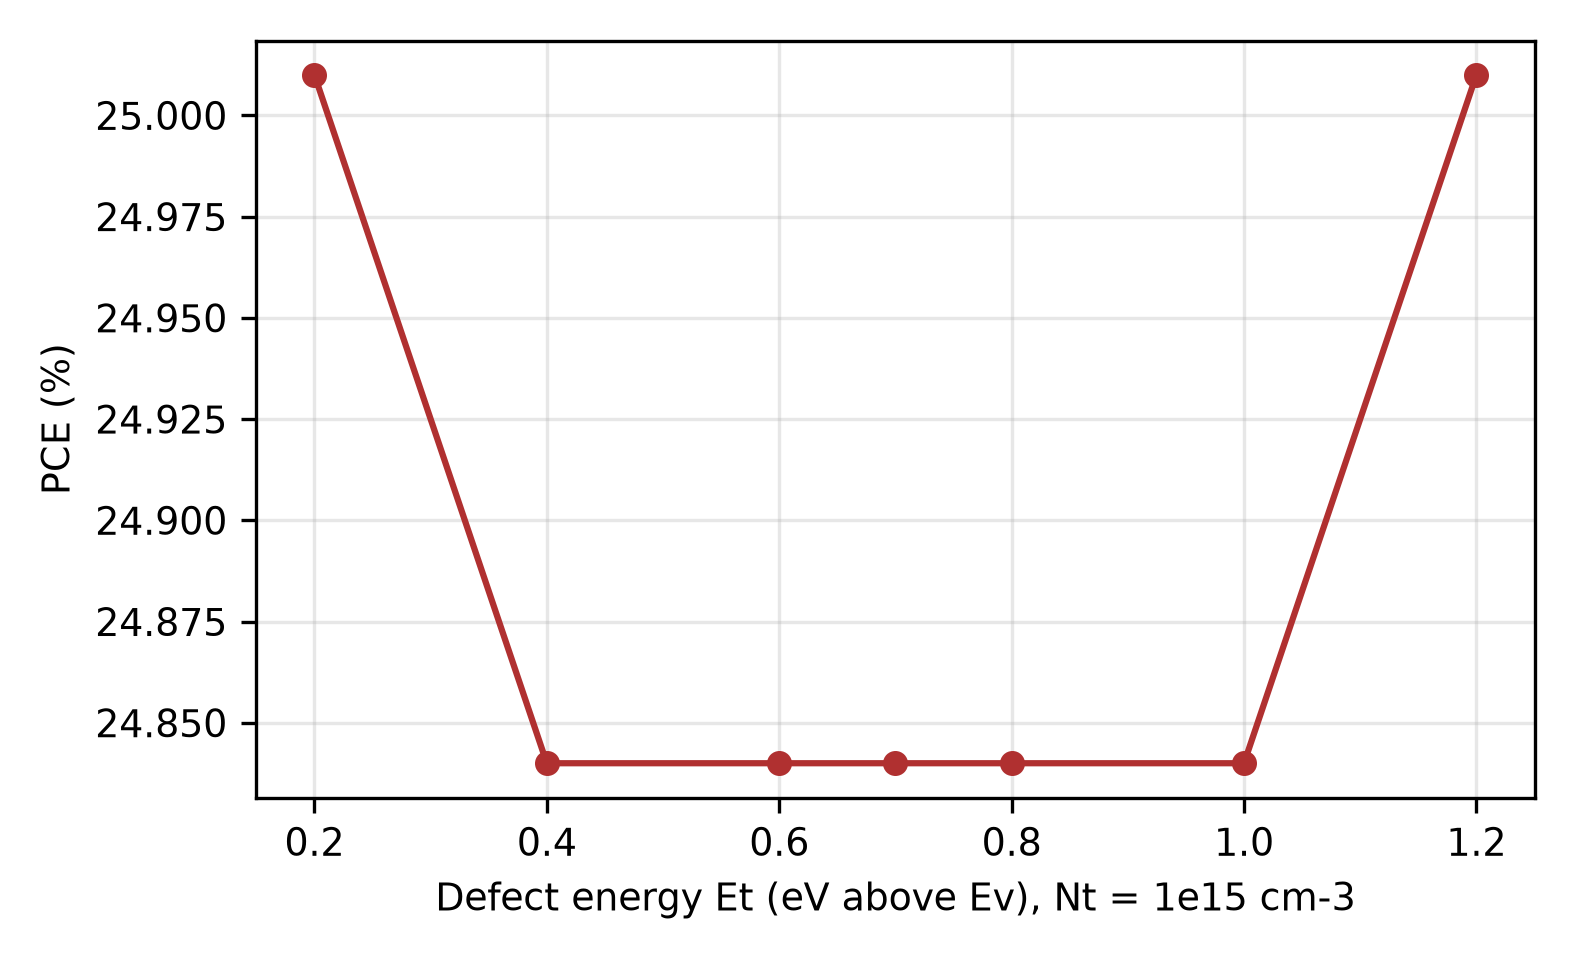
\includegraphics[width=0.85\linewidth]{figs/fig24.png}
\caption{PCE versus defect energy $E_{\mathrm{t}}$ at $N_{\mathrm{t}}$ = $10^{15}$ cm$^{-3}$. Symmetric minimum at mid-gap (24.84\%) recovering to 25.01\% at both band edges: the SRH fingerprint.}
\end{figure}

\begin{figure}[htbp]
\centering
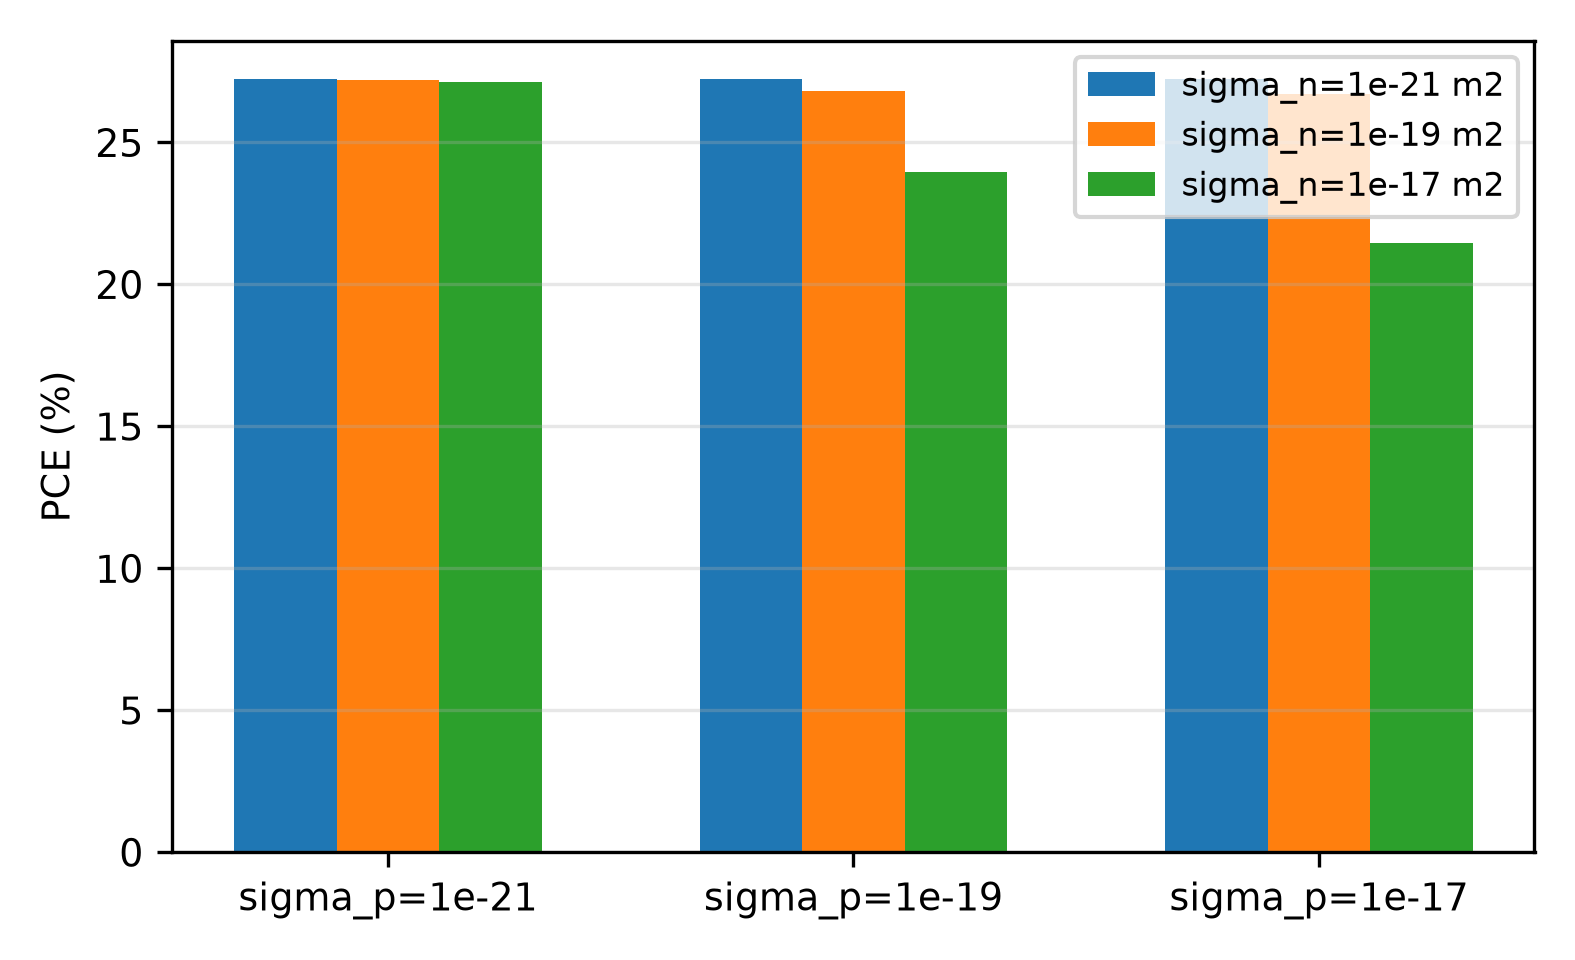
\includegraphics[width=0.85\linewidth]{figs/fig25.png}
\caption{PCE versus capture cross-section asymmetry at mid-gap $E_{\mathrm{t}}$. Lethality requires large sigma on either carrier; at fixed product, electron-dominated traps (23.97\%) beat hole-dominated ones (26.71\%) by 2.7 pp.}
\end{figure}

\begin{figure}[htbp]
\centering
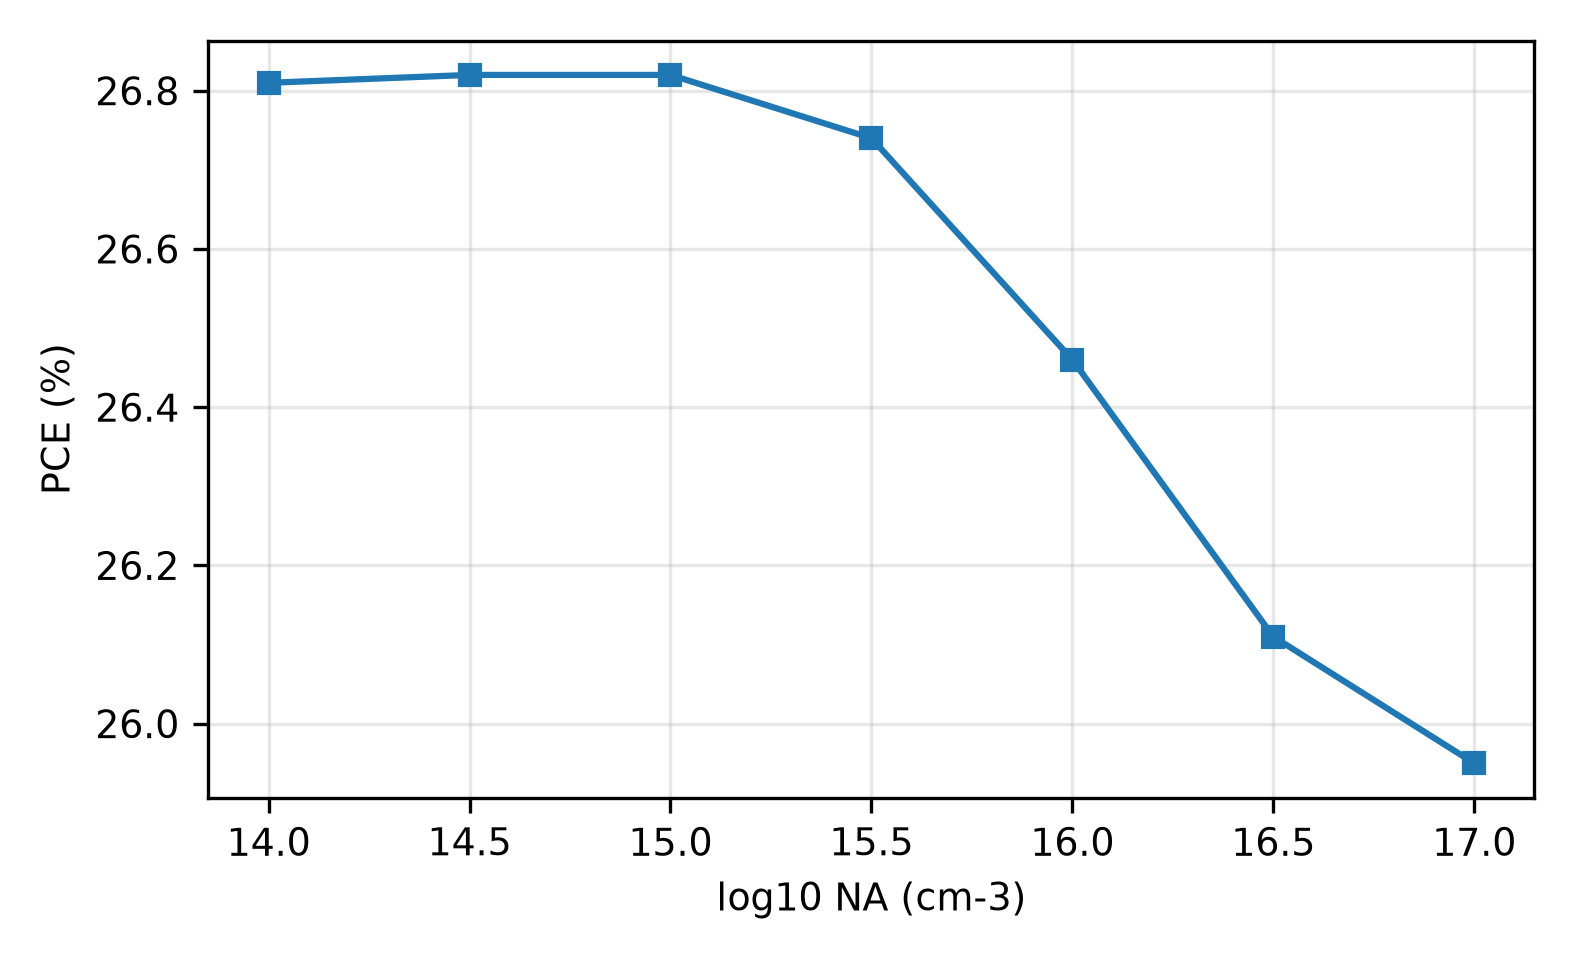
\includegraphics[width=0.85\linewidth]{figs/fig26.png}
\caption{PCE versus background acceptor density. Optimum near $3\times10^{14}$ cm$^{-3}$ (26.82\%); J$_{\mathrm{SC}}$ collapses above $10^{16}$ cm$^{-3}$ while V$_{\mathrm{OC}}$ keeps rising.}
\end{figure}

\begin{figure}[htbp]
\centering
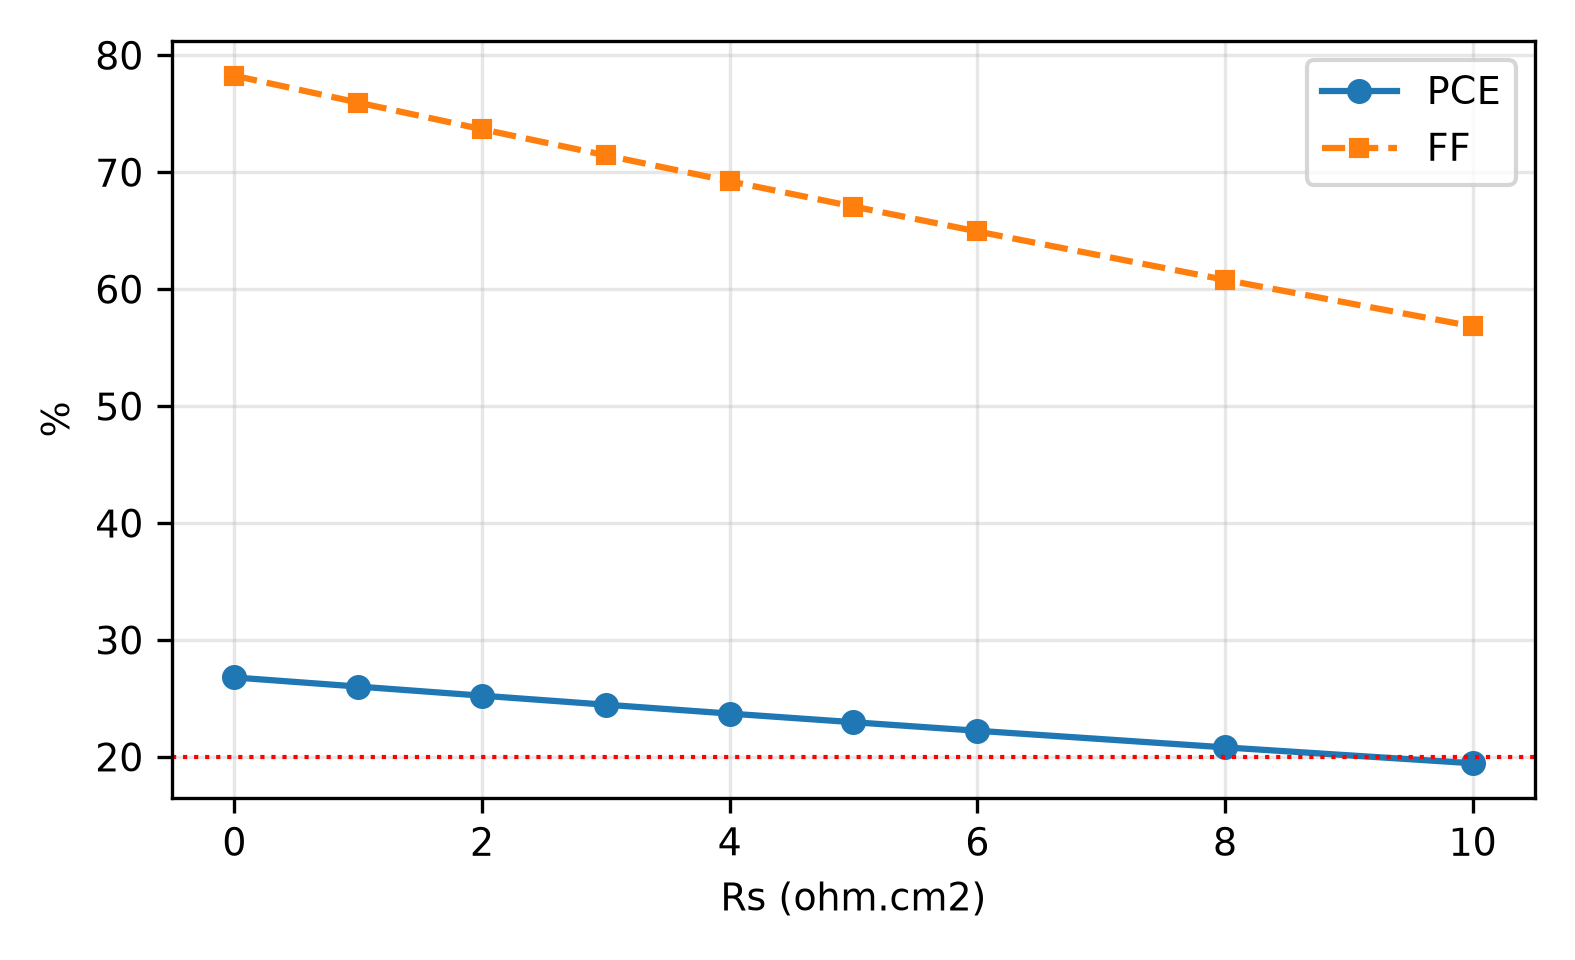
\includegraphics[width=0.85\linewidth]{figs/fig27.png}
\caption{PCE and FF versus series resistance (external V - J x $R_{\mathrm{s}}$ correction). PCE stays above 20\% to $R_{\mathrm{s}}$ = 8 $\Omega\cdot$cm$^{2}$.}
\end{figure}

\begin{figure}[htbp]
\centering
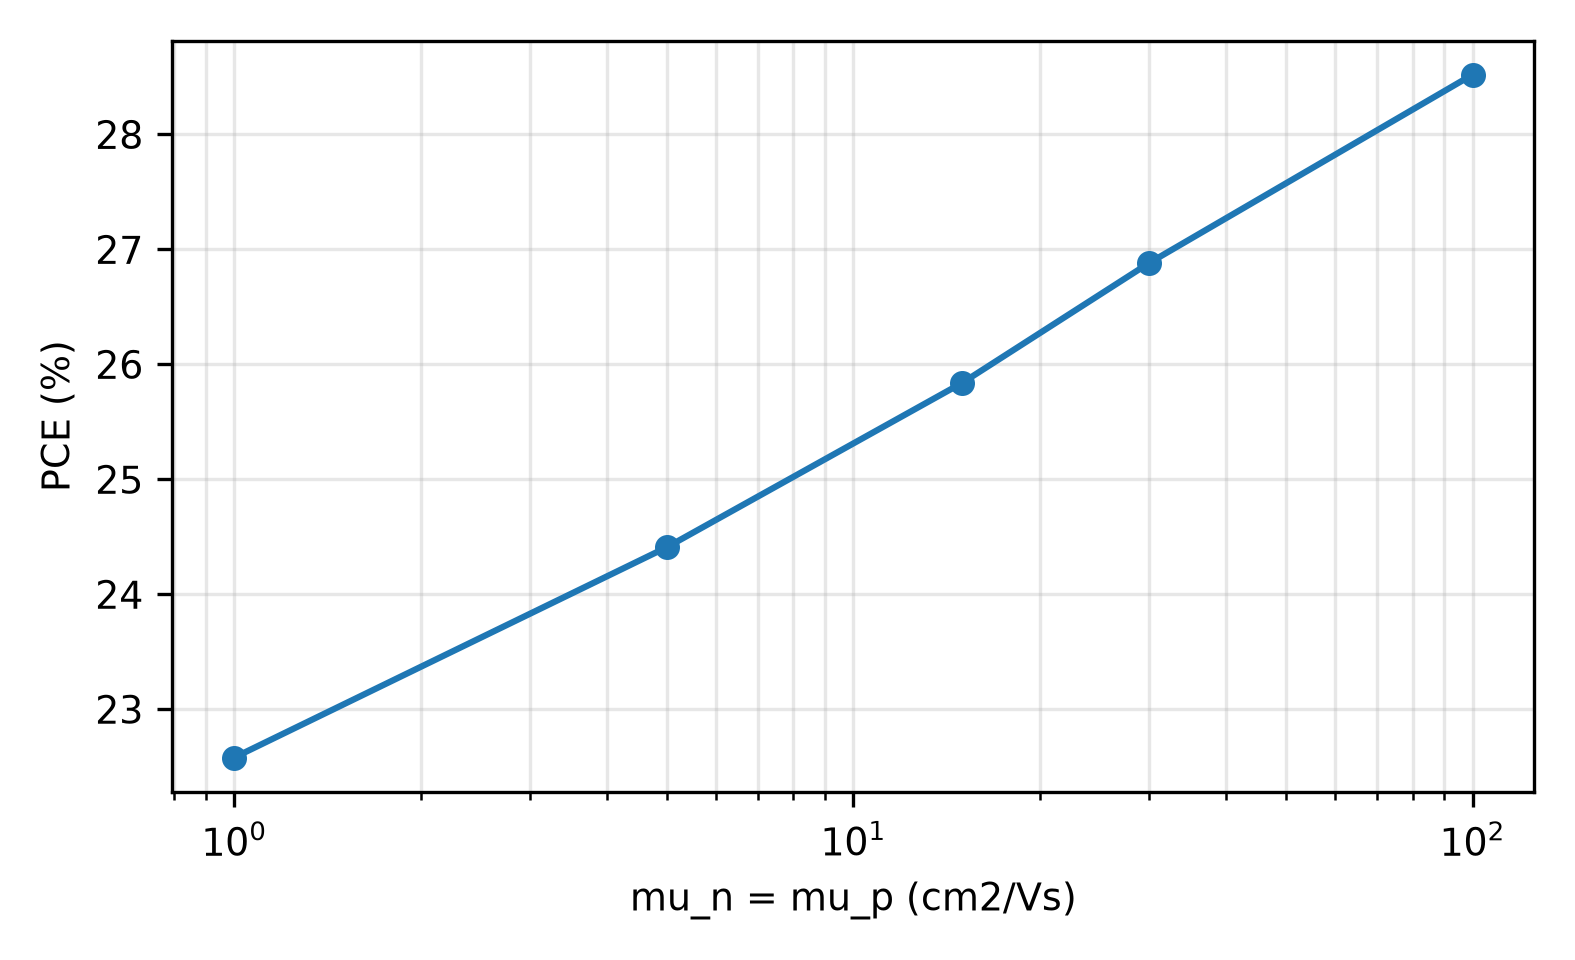
\includegraphics[width=0.85\linewidth]{figs/fig28.png}
\caption{PCE versus absorber mobility ($\mu_{\mathrm{n}}$ = $\mu_{\mathrm{p}}$). Log-linear rise 22.58\% (1) to 28.52\% (100 cm$^{2}$/Vs); target $\mu$ >= 15 cm$^{2}$/Vs.}
\end{figure}

\begin{figure}[htbp]
\centering
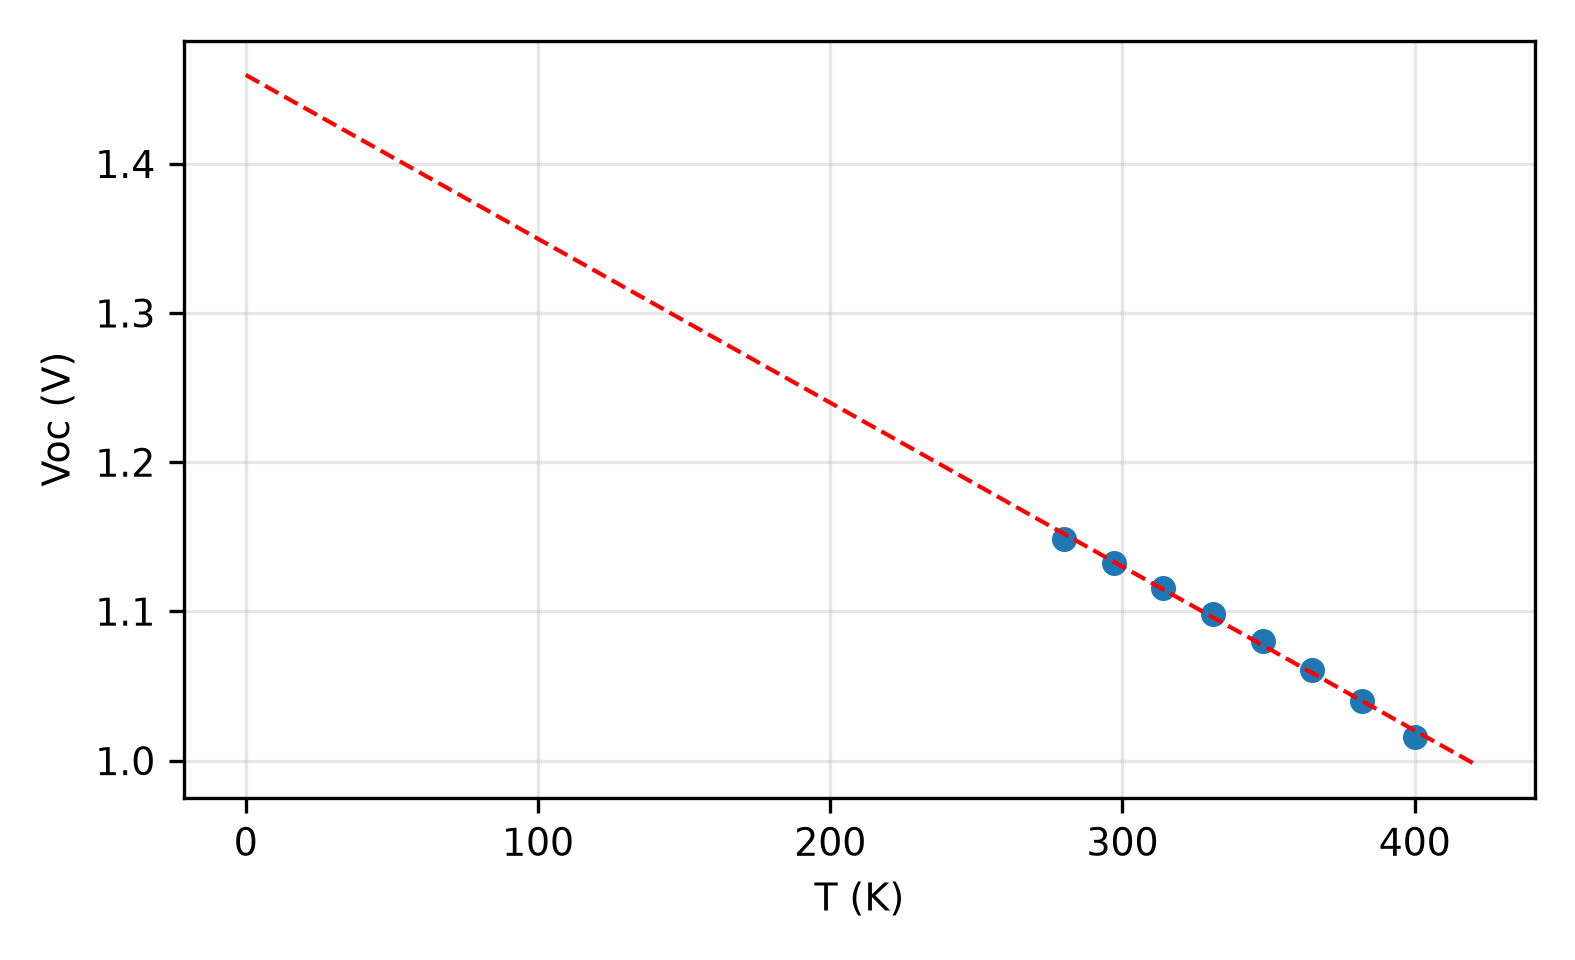
\includegraphics[width=0.85\linewidth]{figs/fig29.png}
\caption{V$_{\mathrm{OC}}$ versus temperature with 0 K extrapolation. $E_{\mathrm{a}}$ = 1.46 eV approx $E_{\mathrm{g}}$ = 1.4 eV: bulk-dominated recombination; dV$_{\mathrm{OC}}$/dT = -1.10 mV/K.}
\end{figure}

\begin{figure}[htbp]
\centering
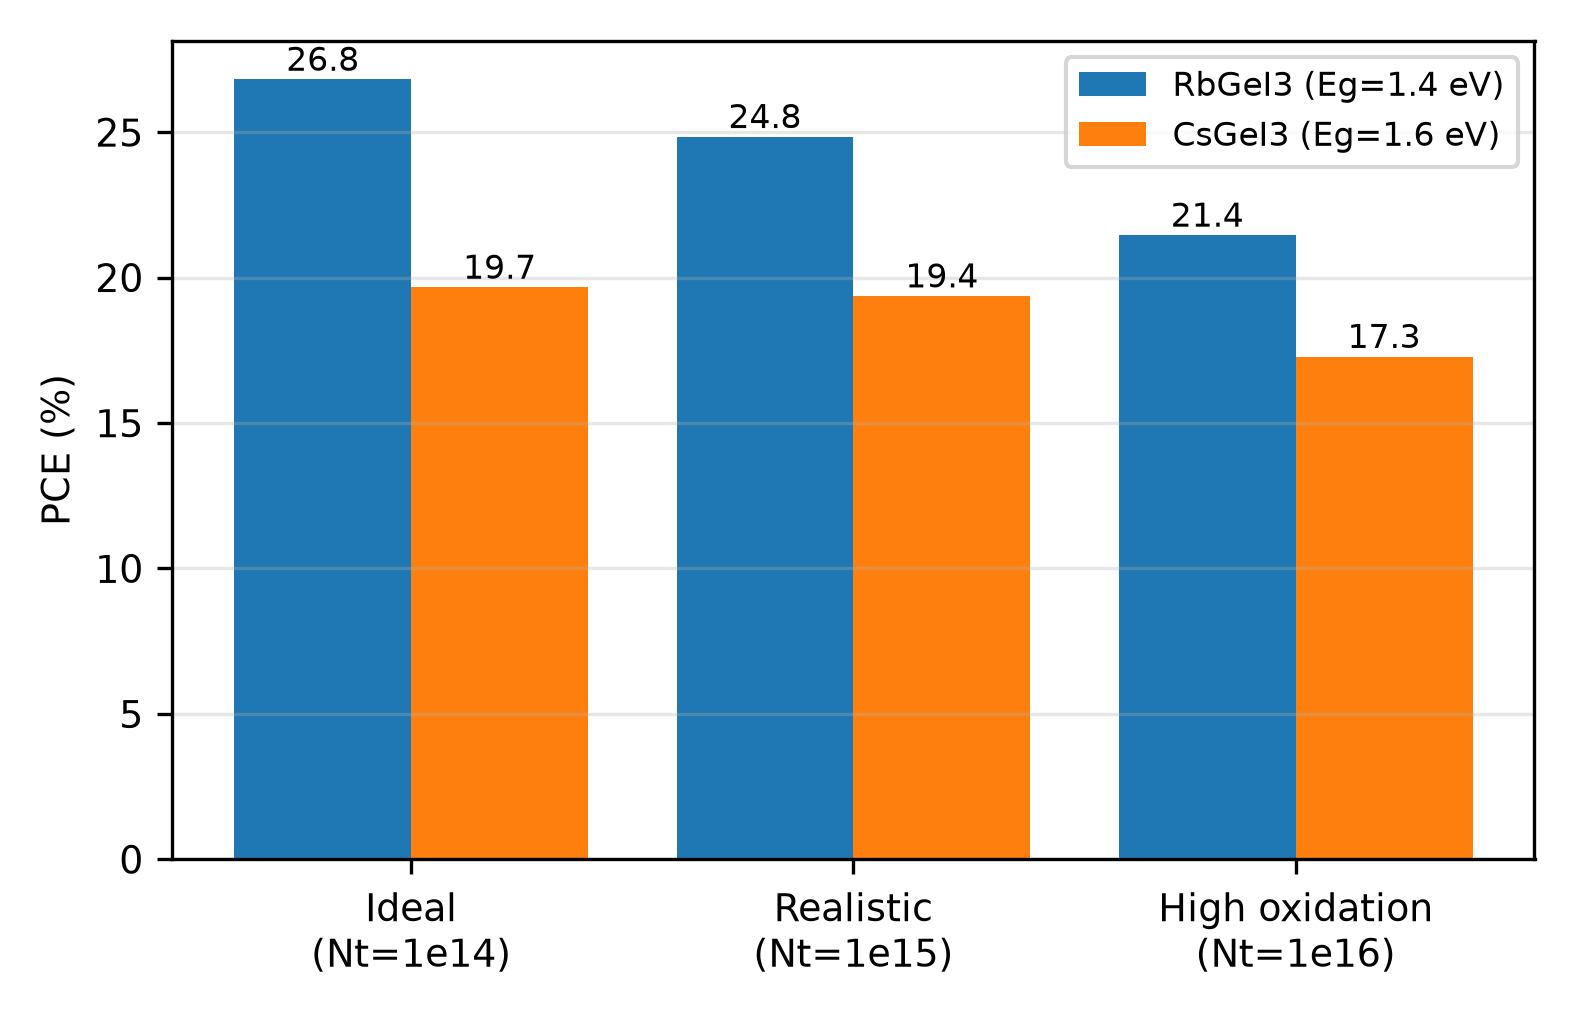
\includegraphics[width=0.85\linewidth]{figs/fig30.png}
\caption{RbGeI$_{3}$ versus CsGeI$_{3}$ under ideal, realistic, and high-oxidation defect budgets in the identical stack. RbGeI$_{3}$ leads at every level.}
\end{figure}

\begin{figure}[htbp]
\centering
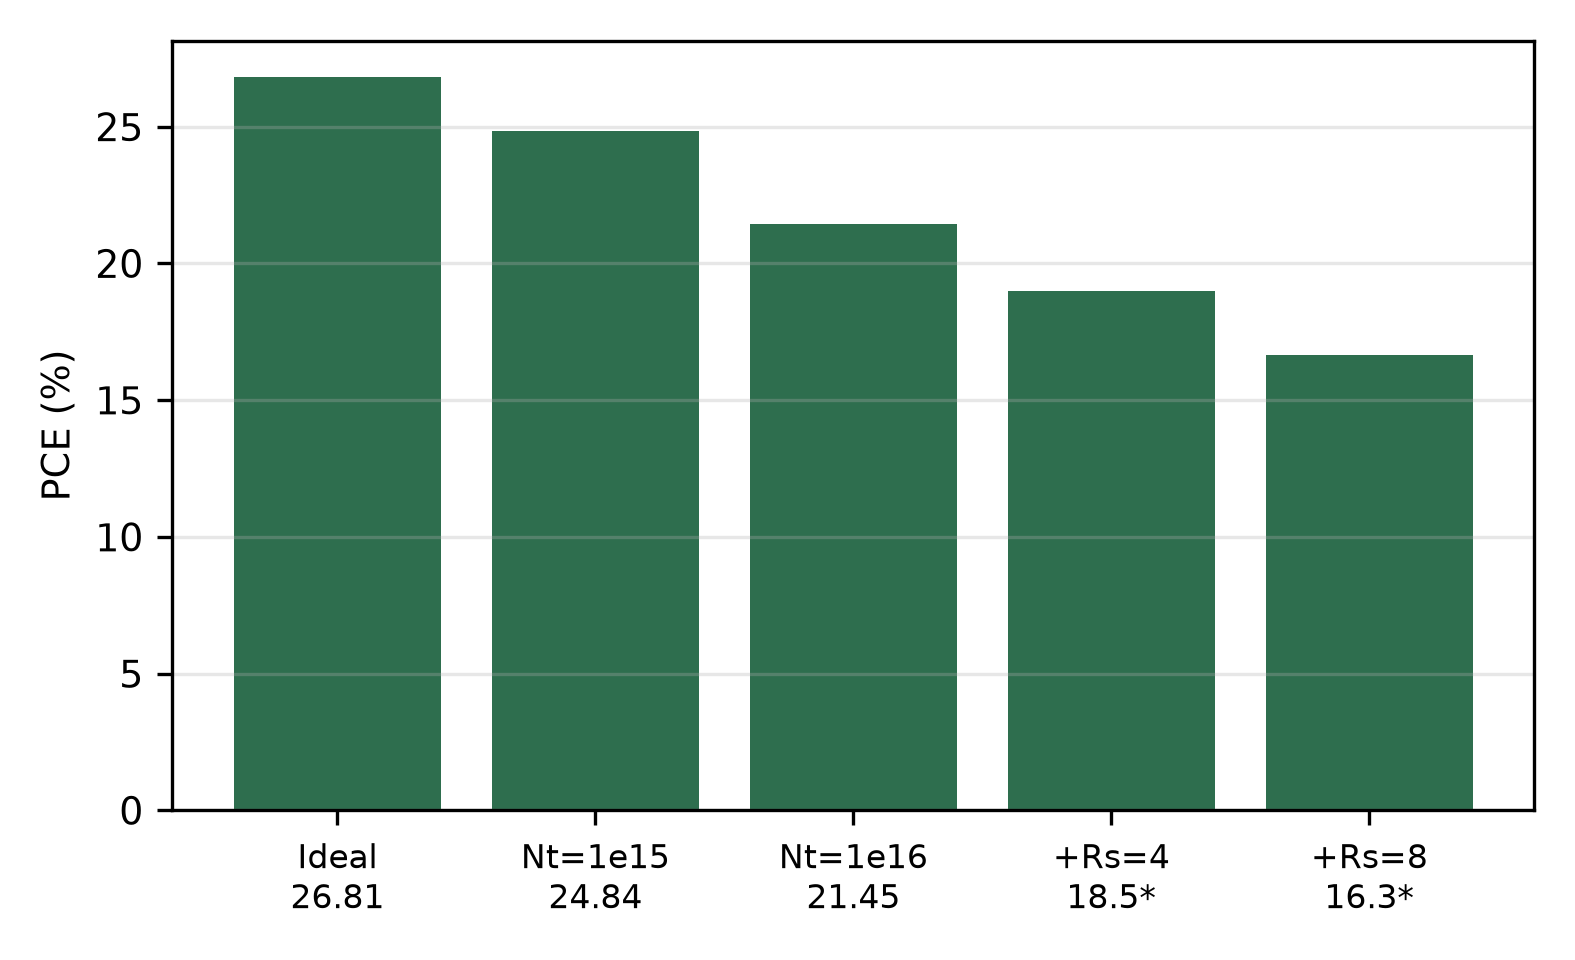
\includegraphics[width=0.85\linewidth]{figs/fig31.png}
\caption{Defect-plus-resistance derating ladder from the 26.81\% ideal point. $R_{\mathrm{s}}$ steps are first-order estimates from the ideal J-V.}
\end{figure}

\section{Limitations and Future Work}

\subsection{Limitations of the present study The defect-plus-resistance ladder measured here bounds the window further: 26.81\% ideal $\rightarrow$ 24.84\% ($N_{\mathrm{t}}$ = $10^{15}$) $\rightarrow$ 21.45\% ($N_{\mathrm{t}}$ = $10^{16}$), with first-order $R_{\mathrm{s}}$ factors giving $\sim$19.0\% ($R_{\mathrm{s}}$ = 4) and $\sim$16.7\% ($R_{\mathrm{s}}$ = 8) at high oxidation (Fig. 31).}
Four caveats bound these results. First, the 26.81\% OPAT device is an ideal-coupling upper bound: a supplementary first-order optical estimate (Fresnel reflection at air/FTO with n $\approx$ 1.93, plus Beer--Lambert parasitic bounds for the 10 nm TiO$_{2}$ and 100 nm CuI layers) lowers J$_{\mathrm{SC}}$ from 30.32 to 26.65 mA/cm$^{2}$ and PCE to 23.49\% (Fig. 23); a full transfer-matrix stack with measured RbGeI$_{3}$ n/k data would refine this further. Second, the assumed defect densities (10$^{14}$ cm$^{-3}$ bulk, 10$^{14}$ cm$^{-2}$ interfaces) require well-passivated films: raising bulk $N_{\mathrm{t}}$ to 10$^{15}$ (10$^{16}$) cm$^{-3}$ drops PCE to 24.84\% (21.45\%), and raising interface $N_{\mathrm{t}}$ to 10$^{15}$ (10$^{16}$) cm$^{-2}$ drops PCE to 23.60\% (18.40\%), with J$_{\mathrm{SC}}$ nearly unchanged and V$_{\mathrm{OC}}$/FF collapsing (Fig. 22). Holding 10$^{14}$ cm$^{-3}$ in RbGeI$_{3}$ is hard because Ge$^{2+}$ oxidizes readily to Ge$^{4+}$ in ambient, creating deep traps. Third, SCAPS-1D assumes uniform composition, abrupt interfaces, and stable parameters that cannot be built exactly; the seven-step absorption grading in the input deck is a numerical profile with no demonstrated deposition recipe (it leaves the J--V unchanged in our re-simulation, so it is kept only as documented input, not as a claimed structure). Fourth, the OPAT sequence misses cross-interactions by construction; the GA joint optimum (31.78\%) shows the mathematical headroom but itself assumes 10$^{12}$ cm$^{-3}$ material that is not demonstrated.

\subsection{Future work}
The obvious next step is to build and test the optimized device under strict inert processing (<0.1 ppm O2/H2O glovebox), with Ge$^{2+}$-stabilizing measures: GeI2-excess or hydrazine-type reducing additives, Lewis-base trap passivation (pyridine/thiourea routes reported for Ge/Sn perovskites), A-site alloying, and encapsulation, followed by long-term stability testing of the RbGeI$_{3}$/CuI stack. On the modelling side, three extensions are queued: (i) a full 11-parameter global optimization (Bayesian or surrogate-assisted, $\approx$500 evaluations) to confirm the six-gene GA maximum; (ii) a transfer-matrix optical model coupled to the drift-diffusion solution using measured RbGeI$_{3}$ n/k spectra; and (iii) replacing the numerical absorption grading with a physically realizable composition grade, e.g. a RbGe(I1$-$xBrx)3 halide gradient or a RbGe1$-$xSnxI3 alloy gradient deposited sequentially, with the graded profile re-optimized in SCAPS.

\section{Conclusion}
We optimized a lead-free RbGeI$_{3}$ perovskite solar cell in SCAPS-1D, with the goal of higher efficiency and no lead in the absorber. RbGeI$_{3}$ is non-toxic and has the optical and electronic properties an absorber needs, which makes it a credible candidate for future photovoltaics.
We started from eight configurations spanning two ETLs (TiO$_{2}$, PCBM) and four HTLs (NiO, CuI, CBTS, Spiro-OMeTAD). FTO/\allowbreak{}TiO$_{2}$/RbGeI$_{3}$/CuI/\allowbreak{}Au won the screening on durability, cost, and hole mobility rather than raw efficiency; its initial PCE was not the best of the eight, and it then held its gains through optimization. Its edge traces to band alignment, efficient charge extraction, low recombination, and clean transport at the interfaces. The choice is explicitly stability- and cost-constrained (CuI durability and cost, TiO$_{2}$ processing), not raw-efficiency-led: D2 (TiO$_{2}$/NiO, 21.10\%) outscored D4 (19.78\%) at screening.
After sequential optimization of eleven parameters, the consolidated device reaches 26.81\% (V$_{\mathrm{OC}}$ = 1.13 V, J$_{\mathrm{SC}}$ = 30.32 mA/cm$^{2}$, FF = 78.26\%), within 0.4 percentage points of the best prior RbGeI$_{3}$ simulation. RbGeI$_{3}$ at 1.4 eV, in short, is a computationally promising absorber candidate subject to the realism bounds above. Joint GA optimization finds a higher joint optimum at 31.78\% ($E_{\mathrm{g}}$ = 1.33 eV, 62 evaluations), while first-order optical derating and realistic defect densities bound the experimentally plausible window to $\approx$20.7--23.5\%. Defect-energy, doping, resistance, mobility, and CsGeI$_{3}$-comparison sweeps (Sections V.C, V.U-W, VI.B) convert the headline into manufacturing tolerances: $E_{\mathrm{a}}$ = 1.46 eV (bulk-limited), $N_{\mathrm{A}}$ <= $10^{15}$ cm$^{-3}$, $R_{\mathrm{s}}$ <= 8 $\Omega\cdot$cm$^{2}$, $\mu$ >= 15 cm$^{2}$/Vs.

\begin{thebibliography}{99}
\bibitem{r1} RENEWABLES 2024 Global Status Report (REN21, 2024).
\bibitem{r2} World Energy Outlook 2024 (International Energy Agency, IEA, 2024).
\bibitem{r3} M. A. Green et al., ``Solar cell efficiency tables (Version 64),'' Prog. Photovolt.: Res. Appl. (2024). doi:\url{10.1002/pip.3831.}
\bibitem{r4} R. A. Afre and D. Pugliese, ``Perovskite solar cells: A review of the latest advances in materials, fabrication techniques, and stability enhancement strategies,'' Micromachines 15(2), 192 (2024). doi:\url{10.3390/mi15020192.}
\bibitem{r5} N.-G. Park, M. Grätzel, T. Miyasaka, K. Zhu, and K. Emery, ``Towards stable and commercially available perovskite solar cells,'' Nat. Energy 1(11), 16152 (2016). doi:\url{10.1038/nenergy.2016.152.}
\bibitem{r6} ``Compositional engineering of perovskite materials for high-performance solar cells,'' Nature 517(7535), 476--480 (2015). doi:\url{10.1038/nature14133.}
\bibitem{r7} I. Ahmed, K. Prakash, and S. M. Mobin, ``Lead-free perovskites for solar cell applications: recent progress, ongoing challenges, and strategic approaches,'' Chem. Commun. 61(37), 6691--6721 (2025). doi:\url{10.1039/D4CC06835A.}
\bibitem{r8} S. Kinza Fatima et al., ``Lead-free perovskites for next-generation applications: a comprehensive computational and data-driven review,'' Mater. Adv. 6(21), 7634--7661 (2025). doi:\url{10.1039/D5MA00681C.}
\bibitem{r9} J. Burschka, N. Pellet, S.-J. Moon, R. Humphry-Baker, P. Gao, M. K. Nazeeruddin, and M. Grätzel, ``Sequential deposition as a route to high-performance perovskite-sensitized solar cells,'' Nature 499(7458), 316--319 (2013). doi:\url{10.1038/nature12340.}
\bibitem{r10} M. M. Lee, J. Teuscher, T. Miyasaka, T. N. Murakami, and H. J. Snaith, ``Efficient hybrid solar cells based on meso-superstructured organometal halide perovskites,'' Science 338(6107), 643--647 (2012). doi:\url{9.7726/science.1228604.}
\bibitem{r11} A. K. Jena, A. Kulkarni, and T. Miyasaka, ``Halide perovskite photovoltaics: Background, status, and future prospects,'' Chem. Rev. 119(5), 3036--3103 (2019). doi:\url{10.1021/acs.chemrev.8b00539.}
\bibitem{r12} P. Afrin, K. Farjana, A. Vumije, and M. N. Uddin, ``An investigation on the impact of temperature variation over the performance of formamidinium tin iodide perovskite solar cell using SCAPS simulation,'' AIP Adv. 14(7) (2024). doi:\url{10.1063/5.0209332.}
\bibitem{r13} S. Samaki, F. Tchangnwa Nya, G. M. Dzifack Kenfack, and A. Laref, ``Materials and interfaces properties optimization for high-efficient and more stable RbGeI$_{3}$ perovskite solar cells: optoelectrical modelling,'' Sci. Rep. 13, 15517 (2023). doi:\url{10.1038/s41598-023-42471-w.}
\bibitem{r14} G. Pindolia, S. M. Shinde, and P. K. Jha, ``Optimization of an inorganic lead-free RbGeI$_{3}$ based perovskite solar cell by SCAPS-1D simulation,'' Sol. Energy 236, 802--821 (2022). doi:\url{10.1016/j.solener.2022.03.053.}
\bibitem{r15} S. Bouazizi, W. Tlili, A. Bouich, B. M. Soucase, and A. Omri, ``Design and efficiency enhancement of FTO/\allowbreak{}PC$_{60}$BM/CsSn0.5Ge0.5I3/\allowbreak{}Spiro-OMeTAD/\allowbreak{}Au perovskite solar cell utilizing SCAPS-1D simulator,'' Mater. Res. Express 9(9), 096402 (2022). doi:\url{10.1088/2053-1591/ac8d52.}
\bibitem{r16} T. Salim, S. Sun, Y. Abe, A. Krishna, A. C. Grimsdale, and Y. M. Lam, ``Perovskite-based solar cells: Impact of materials processing and device architecture,'' J. Mater. Chem. A 3(17), 8943--8969 (2015). doi:\url{10.1039/C4TA05226A.}
\bibitem{r17} P. K. Dash, P. Banarjee, A. Nyayban, and S. Panda, ``Optoelectronic properties and performance optimization for photovoltaic applications of R3m-RbGeX$_{3}$ (X = Cl, Br, I) perovskites: A combined DFT and SCAPS-1D study,'' arXiv:2505.09362 (2025).
\bibitem{r18} N. A. Abdulkareem, ``A DFT study of structural, electronic and optical properties of lead-free and Ge-based cubic perovskite RbGeX$_{3}$ (X = I, Br and Cl),'' Passer J. Basic Appl. Sci. 5(1), 46--51 (2023). doi:\url{10.24271/psr.2023.371069.1187.}
\bibitem{r19} M. Burgelman, P. Nollet, and S. Degrave, ``Modelling polycrystalline semiconductor solar cells,'' Thin Solid Films 361--362, 527--532 (2000). doi:\url{10.1016/S0040-6090(99)00825-1.}
\bibitem{r20} M. Burgelman, M. Debucquoy, K. Decock, J. Verschraegen, and S. Degrave, SCAPS-1D simulation program for thin film solar cells, version 3.3.10 (ELIS, University of Gent, Belgium, 2024).
\bibitem{r21} A. Nakane, H. Tampo, M. Tamakoshi, S. Fujimoto, K. M. Kim, S. Kim, H. Shibata, S. Niki, and H. Fujiwara, ``Quantitative determination of optical and recombination losses in thin-film photovoltaic devices based on external quantum efficiency analysis,'' arXiv:1604.04491 (2016); published in J. Appl. Phys. 120, 064505 (2016), doi:\url{10.1063/1.4960698.}
\bibitem{r22} L. Loumachi, A. Yousfi, O. Saidani, and A. S. Alsubaie, ``Strengthen the power conversion efficiency of solar cell based RbGeI$_{3}$: Numerical approach,'' East Eur. J. Phys. (3), 416--424 (2024). doi:\url{10.26565/2312-4334-2024-3-50}
\bibitem{r23} A. Pathak, K. M. D. Pravalli, R. Madaka, B. Pandey, D. Shankar, C. S. Beera, and D. J. Rao, ``Computational analysis of germanium-based perovskites (MAGeI$_{3}$, FAGeI$_{3}$, CsGeI$_{3}$, RbGeI$_{3}$) for high-efficiency solar cells using SCAPS-1D,'' Research Square (2026). doi:\url{10.21203/rs.3.rs-8749975/}
\bibitem{r24} D. Saikia, J. Bera, A. Betal, and S. Sahu, ``Performance evaluation of an all inorganic CsGeI$_{3}$ based perovskite solar cell by numerical simulation,'' Opt. Mater. 123, 111839 (2022). doi:\url{10.1016/j.optmat.2021.111839.}
\bibitem{r25} R. Pau et al., ``Solution-processed CuI as a hole transport layer for Sn--Pb perovskite solar cells,'' J. Mater. Chem. A 13(48), 42118--42127 (2025). doi:\url{10.1039/D5TA06770G.}
\bibitem{r26} Q. Sun, A. Sadhu, S. Lie, and L. H. Wong, ``Critical review of Cu-based hole transport materials for perovskite solar cells: From theoretical insights to experimental validation,'' Adv. Mater. (2024). doi:\url{10.1002/adma.202402412.}
\bibitem{r27} J. Z. Mbese, ``Advancements in inorganic hole-transport materials for perovskite solar cells: A comparative review,'' Energies 18(9), 2374 (2025). doi:\url{10.3390/en18092374.}
\bibitem{r28} L. T. C. Tuyen, S.-R. Jian, N. T. Tien, and P. H. Le, ``Nanomechanical and material properties of fluorine-doped tin oxide thin films prepared by ultrasonic spray pyrolysis: Effects of F-doping,'' Materials 12(10), 1665 (2019). doi:\url{10.3390/ma12101665.}
\bibitem{r29} W. Yang et al., ``The CuI/\allowbreak{}NiO gradient hole transport layer for enhanced carrier efficiency in large-area perovskite solar cell,'' Appl. Phys. Lett. 128(14) (2026). doi:\url{10.1063/5.0326539.}
\bibitem{r30} A. J. Olasoji and S. H. Im, ``Perspective chapter: TiO$_{2}$ electron transporting layers for perovskite solar cells,'' in Titanium Dioxide -- Uses, Applications, and Advances (IntechOpen, 2024). doi:\url{10.5772/intechopen.1007266.}
\bibitem{r31} K. Valadi, S. Gharibi, R. Taheri-Ledari, S. Akin, A. Maleki, and A. E. Shalan, ``Metal oxide electron transport materials for perovskite solar cells: A review,'' Environ. Chem. Lett. 19(3), 2185--2207 (2021). doi:\url{10.1007/s10311-020-01171-x.}
\bibitem{r32} L. Ji, T. Zhang, and S. Li, ``Band alignment of TiO$_{2}$ by controlling Cl content for high-efficiency perovskite solar cells,'' J. Mater. Chem. C 12(36), 14597--14604 (2024). doi:\url{10.1039/D4TC01495B.}
\bibitem{r33} A. Ghosh et al., ``Solar power conversion: CuI hole transport layer and Ba3NCl3 absorber enable advanced solar cell technology boosting efficiency over 30\%,'' RSC Adv. 14(33), 24066--24081 (2024). doi:\url{10.1039/D4RA03695F.}
\bibitem{r34} T. Minemoto and M. Murata, ``Impact of work function of back contact of perovskite solar cells without hole transport material analyzed by device simulation,'' Curr. Appl. Phys. 14(11), 1428--1433 (2014). doi:\url{10.1016/j.cap.2014.08.002.}
\bibitem{r35} W. Shockley and H. J. Queisser, ``Detailed balance limit of efficiency of p-n junction solar cells,'' J. Appl. Phys. 32(3), 510--519 (1961). doi:\url{10.1063/1.1736034.}
\bibitem{r36} S. Rühle, ``Tabulated values of the Shockley--Queisser limit for single junction solar cells,'' Sol. Energy 130, 139--147 (2016). doi:\url{10.1016/j.solener.2016.02.015.}
\bibitem{r37} C. H. Henry, ``Limiting efficiencies of ideal single and multiple energy gap terrestrial solar cells,'' J. Appl. Phys. 51(8), 4494--4500 (1980). doi:\url{10.1063/1.328272.}
\bibitem{r38} O. J. Sandberg and A. Armin, ``On the effect of surface recombination in thin film solar cells, light emitting diodes and photodetectors,'' arXiv:1905.07291 (2019); published in Synth. Met. 254, 114--121 (2019), doi:\url{10.1016/j.synthmet.2019.06.008.}
\bibitem{r39} M. Raj, A. Aggarwal, A. Kushwaha, and N. Goel, ``Moisture-resistant sustainable solar cell with RbGeI$_{3}$ absorber layer,'' J. Mater. Sci. 60(22), 9176--9196 (2025). doi:\url{10.1007/s10853-025-11002-5.}
\bibitem{r40} H.-J. Park, H. Son, and B.-S. Jeong, ``SCAPS-1D Simulation for Device Optimization to Improve Efficiency in Lead-Free CsSnI$_{3}$ Perovskite Solar Cells,'' Inorganics 12(4), 123 (2024). doi:\url{10.3390/inorganics12040123.}
\bibitem{r41} R. Islam, M. N. Uddin, M. J. Hossen, and A. Begum, ``Photovoltaic performance of lead-free MASnI$_{3}$-based perovskite solar cells with kesterite hole transport materials,'' AIP Adv. 16(5) (2026). doi:\url{10.1063/5.0315071.}
\bibitem{r42} A. C. Piñón Reyes et al., ``Study of a lead-free perovskite solar cell using CZTS as HTL to achieve a 20\% PCE by SCAPS-1D simulation,'' Micromachines 12(12), 1508 (2021). doi:\url{10.3390/mi12121508.}
\end{thebibliography}
\end{document}